\documentclass[12pt,letter]{article}
%%%%%%%%%%%%%%%%%%%%%%%%%%%%%%%%%%%%%%%%%%%%%%%%%%%%%%%%%%%%%%%%%%%%%%%%%%%%%%%%
\usepackage{booktabs, caption, subcaption, float}
\usepackage[latin1]{inputenc}
\usepackage{longtable}
\usepackage{graphics}
\usepackage{geometry}
\usepackage{graphicx}
\usepackage{amsfonts, amssymb, amsmath}
\usepackage{natbib, multibib}
\usepackage{theorem}
\usepackage{setspace}
\usepackage[normalem]{ulem}
\usepackage{caption}
\usepackage{tabularx}
\usepackage{epstopdf}
\usepackage{rotating}
\usepackage{placeins}
\usepackage[makeroom]{cancel}
\usepackage{varioref}
\usepackage{hyperref}

\setcounter{MaxMatrixCols}{10}
% TCIDATA{OutputFilter=Latex.dll} TCIDATA{Version=5.50.0.2960}
% TCIDATA{<META NAME="SaveForMode" CONTENT="1">}
% TCIDATA{BibliographyScheme=BibTeX} TCIDATA{LastRevised=Monday, May
% 11, 2015 19:08:26} TCIDATA{<META NAME="GraphicsSave" CONTENT="32">}

\theoremstyle{break} \theorembodyfont{\normalfont\itshape}
\newtheorem{thm}{Theorem}
\theoremstyle{break}
\theorembodyfont{\normalfont\itshape}
\newtheorem{corrollary}{Corollary} \theoremstyle{break}
\theorembodyfont{\normalfont\itshape} \newtheorem{prop}{Proposition}
\theoremstyle{break} \theorembodyfont{\normalfont\itshape}
\newtheorem{lemma}{Lemma} \theoremstyle{break}
\theorembodyfont{\normalfont\itshape} \newtheorem{algm}{Algorithm}
\theoremstyle{break} \theorembodyfont{\normalfont\itshape}
\newtheorem{definition}{Definition} \theoremstyle{break}
\theorembodyfont{\normalfont\itshape}
\newtheorem{condition}{Condition} \theoremstyle{break}
\theorembodyfont{\normalfont\itshape}

\renewcommand{\baselinestretch}{1.5}
\setlength{\hoffset}{-0.4in}
\setlength{\textwidth}{6.8in}
\setlength{\textheight}{9.3in}
\setlength{\topmargin}{-0.5in}
% Macros for Scientific Word and Scientific WorkPlace 5.5 documents saved with the LaTeX filter.
% Copyright (C) 2005 Mackichan Software, Inc.

\typeout{TCILATEX Macros for Scientific Word and Scientific WorkPlace 5.5 <06 Oct 2005>.}
\typeout{NOTICE:  This macro file is NOT proprietary and may be 
freely copied and distributed.}
%
\makeatletter

%%%%%%%%%%%%%%%%%%%%%
% pdfTeX related.
\ifx\pdfoutput\relax\let\pdfoutput=\undefined\fi
\newcount\msipdfoutput
\ifx\pdfoutput\undefined
\else
 \ifcase\pdfoutput
 \else 
    \msipdfoutput=1
    \ifx\paperwidth\undefined
    \else
      \ifdim\paperheight=0pt\relax
      \else
        \pdfpageheight\paperheight
      \fi
      \ifdim\paperwidth=0pt\relax
      \else
        \pdfpagewidth\paperwidth
      \fi
    \fi
  \fi  
\fi

%%%%%%%%%%%%%%%%%%%%%
% FMTeXButton
% This is used for putting TeXButtons in the 
% frontmatter of a document. Add a line like
% \QTagDef{FMTeXButton}{101}{} to the filter 
% section of the cst being used. Also add a
% new section containing:
%     [f_101]
%     ALIAS=FMTexButton
%     TAG_TYPE=FIELD
%     TAG_LEADIN=TeX Button:
%
% It also works to put \defs in the preamble after 
% the \input tcilatex
\def\FMTeXButton#1{#1}
%
%%%%%%%%%%%%%%%%%%%%%%
% macros for time
\newcount\@hour\newcount\@minute\chardef\@x10\chardef\@xv60
\def\tcitime{
\def\@time{%
  \@minute\time\@hour\@minute\divide\@hour\@xv
  \ifnum\@hour<\@x 0\fi\the\@hour:%
  \multiply\@hour\@xv\advance\@minute-\@hour
  \ifnum\@minute<\@x 0\fi\the\@minute
  }}%

%%%%%%%%%%%%%%%%%%%%%%
% macro for hyperref and msihyperref
%\@ifundefined{hyperref}{\def\hyperref#1#2#3#4{#2\ref{#4}#3}}{}

\def\x@hyperref#1#2#3{%
   % Turn off various catcodes before reading parameter 4
   \catcode`\~ = 12
   \catcode`\$ = 12
   \catcode`\_ = 12
   \catcode`\# = 12
   \catcode`\& = 12
   \catcode`\% = 12
   \y@hyperref{#1}{#2}{#3}%
}

\def\y@hyperref#1#2#3#4{%
   #2\ref{#4}#3
   \catcode`\~ = 13
   \catcode`\$ = 3
   \catcode`\_ = 8
   \catcode`\# = 6
   \catcode`\& = 4
   \catcode`\% = 14
}

\@ifundefined{hyperref}{\let\hyperref\x@hyperref}{}
\@ifundefined{msihyperref}{\let\msihyperref\x@hyperref}{}




% macro for external program call
\@ifundefined{qExtProgCall}{\def\qExtProgCall#1#2#3#4#5#6{\relax}}{}
%%%%%%%%%%%%%%%%%%%%%%
%
% macros for graphics
%
\def\FILENAME#1{#1}%
%
\def\QCTOpt[#1]#2{%
  \def\QCTOptB{#1}
  \def\QCTOptA{#2}
}
\def\QCTNOpt#1{%
  \def\QCTOptA{#1}
  \let\QCTOptB\empty
}
\def\Qct{%
  \@ifnextchar[{%
    \QCTOpt}{\QCTNOpt}
}
\def\QCBOpt[#1]#2{%
  \def\QCBOptB{#1}%
  \def\QCBOptA{#2}%
}
\def\QCBNOpt#1{%
  \def\QCBOptA{#1}%
  \let\QCBOptB\empty
}
\def\Qcb{%
  \@ifnextchar[{%
    \QCBOpt}{\QCBNOpt}%
}
\def\PrepCapArgs{%
  \ifx\QCBOptA\empty
    \ifx\QCTOptA\empty
      {}%
    \else
      \ifx\QCTOptB\empty
        {\QCTOptA}%
      \else
        [\QCTOptB]{\QCTOptA}%
      \fi
    \fi
  \else
    \ifx\QCBOptA\empty
      {}%
    \else
      \ifx\QCBOptB\empty
        {\QCBOptA}%
      \else
        [\QCBOptB]{\QCBOptA}%
      \fi
    \fi
  \fi
}
\newcount\GRAPHICSTYPE
%\GRAPHICSTYPE 0 is for TurboTeX
%\GRAPHICSTYPE 1 is for DVIWindo (PostScript)
%%%(removed)%\GRAPHICSTYPE 2 is for psfig (PostScript)
\GRAPHICSTYPE=\z@
\def\GRAPHICSPS#1{%
 \ifcase\GRAPHICSTYPE%\GRAPHICSTYPE=0
   \special{ps: #1}%
 \or%\GRAPHICSTYPE=1
   \special{language "PS", include "#1"}%
%%%\or%\GRAPHICSTYPE=2
%%%  #1%
 \fi
}%
%
\def\GRAPHICSHP#1{\special{include #1}}%
%
% \graffile{ body }                                  %#1
%          { contentswidth (scalar)  }               %#2
%          { contentsheight (scalar) }               %#3
%          { vertical shift when in-line (scalar) }  %#4

\def\graffile#1#2#3#4{%
%%% \ifnum\GRAPHICSTYPE=\tw@
%%%  %Following if using psfig
%%%  \@ifundefined{psfig}{\input psfig.tex}{}%
%%%  \psfig{file=#1, height=#3, width=#2}%
%%% \else
  %Following for all others
  % JCS - added BOXTHEFRAME, see below
    \bgroup
	   \@inlabelfalse
       \leavevmode
       \@ifundefined{bbl@deactivate}{\def~{\string~}}{\activesoff}%
        \raise -#4 \BOXTHEFRAME{%
           \hbox to #2{\raise #3\hbox to #2{\null #1\hfil}}}%
    \egroup
}%
%
% A box for drafts
\def\draftbox#1#2#3#4{%
 \leavevmode\raise -#4 \hbox{%
  \frame{\rlap{\protect\tiny #1}\hbox to #2%
   {\vrule height#3 width\z@ depth\z@\hfil}%
  }%
 }%
}%
%
\newcount\@msidraft
\@msidraft=\z@
\let\nographics=\@msidraft
\newif\ifwasdraft
\wasdraftfalse

%  \GRAPHIC{ body }                                  %#1
%          { draft name }                            %#2
%          { contentswidth (scalar)  }               %#3
%          { contentsheight (scalar) }               %#4
%          { vertical shift when in-line (scalar) }  %#5
\def\GRAPHIC#1#2#3#4#5{%
   \ifnum\@msidraft=\@ne\draftbox{#2}{#3}{#4}{#5}%
   \else\graffile{#1}{#3}{#4}{#5}%
   \fi
}
%
\def\addtoLaTeXparams#1{%
    \edef\LaTeXparams{\LaTeXparams #1}}%
%
% JCS -  added a switch BoxFrame that can 
% be set by including X in the frame params.
% If set a box is drawn around the frame.

\newif\ifBoxFrame \BoxFramefalse
\newif\ifOverFrame \OverFramefalse
\newif\ifUnderFrame \UnderFramefalse

\def\BOXTHEFRAME#1{%
   \hbox{%
      \ifBoxFrame
         \frame{#1}%
      \else
         {#1}%
      \fi
   }%
}


\def\doFRAMEparams#1{\BoxFramefalse\OverFramefalse\UnderFramefalse\readFRAMEparams#1\end}%
\def\readFRAMEparams#1{%
 \ifx#1\end%
  \let\next=\relax
  \else
  \ifx#1i\dispkind=\z@\fi
  \ifx#1d\dispkind=\@ne\fi
  \ifx#1f\dispkind=\tw@\fi
  \ifx#1t\addtoLaTeXparams{t}\fi
  \ifx#1b\addtoLaTeXparams{b}\fi
  \ifx#1p\addtoLaTeXparams{p}\fi
  \ifx#1h\addtoLaTeXparams{h}\fi
  \ifx#1X\BoxFrametrue\fi
  \ifx#1O\OverFrametrue\fi
  \ifx#1U\UnderFrametrue\fi
  \ifx#1w
    \ifnum\@msidraft=1\wasdrafttrue\else\wasdraftfalse\fi
    \@msidraft=\@ne
  \fi
  \let\next=\readFRAMEparams
  \fi
 \next
 }%
%
%Macro for In-line graphics object
%   \IFRAME{ contentswidth (scalar)  }               %#1
%          { contentsheight (scalar) }               %#2
%          { vertical shift when in-line (scalar) }  %#3
%          { draft name }                            %#4
%          { body }                                  %#5
%          { caption}                                %#6


\def\IFRAME#1#2#3#4#5#6{%
      \bgroup
      \let\QCTOptA\empty
      \let\QCTOptB\empty
      \let\QCBOptA\empty
      \let\QCBOptB\empty
      #6%
      \parindent=0pt
      \leftskip=0pt
      \rightskip=0pt
      \setbox0=\hbox{\QCBOptA}%
      \@tempdima=#1\relax
      \ifOverFrame
          % Do this later
          \typeout{This is not implemented yet}%
          \show\HELP
      \else
         \ifdim\wd0>\@tempdima
            \advance\@tempdima by \@tempdima
            \ifdim\wd0 >\@tempdima
               \setbox1 =\vbox{%
                  \unskip\hbox to \@tempdima{\hfill\GRAPHIC{#5}{#4}{#1}{#2}{#3}\hfill}%
                  \unskip\hbox to \@tempdima{\parbox[b]{\@tempdima}{\QCBOptA}}%
               }%
               \wd1=\@tempdima
            \else
               \textwidth=\wd0
               \setbox1 =\vbox{%
                 \noindent\hbox to \wd0{\hfill\GRAPHIC{#5}{#4}{#1}{#2}{#3}\hfill}\\%
                 \noindent\hbox{\QCBOptA}%
               }%
               \wd1=\wd0
            \fi
         \else
            \ifdim\wd0>0pt
              \hsize=\@tempdima
              \setbox1=\vbox{%
                \unskip\GRAPHIC{#5}{#4}{#1}{#2}{0pt}%
                \break
                \unskip\hbox to \@tempdima{\hfill \QCBOptA\hfill}%
              }%
              \wd1=\@tempdima
           \else
              \hsize=\@tempdima
              \setbox1=\vbox{%
                \unskip\GRAPHIC{#5}{#4}{#1}{#2}{0pt}%
              }%
              \wd1=\@tempdima
           \fi
         \fi
         \@tempdimb=\ht1
         %\advance\@tempdimb by \dp1
         \advance\@tempdimb by -#2
         \advance\@tempdimb by #3
         \leavevmode
         \raise -\@tempdimb \hbox{\box1}%
      \fi
      \egroup%
}%
%
%Macro for Display graphics object
%   \DFRAME{ contentswidth (scalar)  }               %#1
%          { contentsheight (scalar) }               %#2
%          { draft label }                           %#3
%          { name }                                  %#4
%          { caption}                                %#5
\def\DFRAME#1#2#3#4#5{%
  \vspace\topsep
  \hfil\break
  \bgroup
     \leftskip\@flushglue
	 \rightskip\@flushglue
	 \parindent\z@
	 \parfillskip\z@skip
     \let\QCTOptA\empty
     \let\QCTOptB\empty
     \let\QCBOptA\empty
     \let\QCBOptB\empty
	 \vbox\bgroup
        \ifOverFrame 
           #5\QCTOptA\par
        \fi
        \GRAPHIC{#4}{#3}{#1}{#2}{\z@}%
        \ifUnderFrame 
           \break#5\QCBOptA
        \fi
	 \egroup
  \egroup
  \vspace\topsep
  \break
}%
%
%Macro for Floating graphic object
%   \FFRAME{ framedata f|i tbph x F|T }              %#1
%          { contentswidth (scalar)  }               %#2
%          { contentsheight (scalar) }               %#3
%          { caption }                               %#4
%          { label }                                 %#5
%          { draft name }                            %#6
%          { body }                                  %#7
\def\FFRAME#1#2#3#4#5#6#7{%
 %If float.sty loaded and float option is 'h', change to 'H'  (gp) 1998/09/05
  \@ifundefined{floatstyle}
    {%floatstyle undefined (and float.sty not present), no change
     \begin{figure}[#1]%
    }
    {%floatstyle DEFINED
	 \ifx#1h%Only the h parameter, change to H
      \begin{figure}[H]%
	 \else
      \begin{figure}[#1]%
	 \fi
	}
  \let\QCTOptA\empty
  \let\QCTOptB\empty
  \let\QCBOptA\empty
  \let\QCBOptB\empty
  \ifOverFrame
    #4
    \ifx\QCTOptA\empty
    \else
      \ifx\QCTOptB\empty
        \caption{\QCTOptA}%
      \else
        \caption[\QCTOptB]{\QCTOptA}%
      \fi
    \fi
    \ifUnderFrame\else
      \label{#5}%
    \fi
  \else
    \UnderFrametrue%
  \fi
  \begin{center}\GRAPHIC{#7}{#6}{#2}{#3}{\z@}\end{center}%
  \ifUnderFrame
    #4
    \ifx\QCBOptA\empty
      \caption{}%
    \else
      \ifx\QCBOptB\empty
        \caption{\QCBOptA}%
      \else
        \caption[\QCBOptB]{\QCBOptA}%
      \fi
    \fi
    \label{#5}%
  \fi
  \end{figure}%
 }%
%
%
%    \FRAME{ framedata f|i tbph x F|T }              %#1
%          { contentswidth (scalar)  }               %#2
%          { contentsheight (scalar) }               %#3
%          { vertical shift when in-line (scalar) }  %#4
%          { caption }                               %#5
%          { label }                                 %#6
%          { name }                                  %#7
%          { body }                                  %#8
%
%    framedata is a string which can contain the following
%    characters: idftbphxFT
%    Their meaning is as follows:
%             i, d or f : in-line, display, or floating
%             t,b,p,h   : LaTeX floating placement options
%             x         : fit contents box to contents
%             F or T    : Figure or Table. 
%                         Later this can expand
%                         to a more general float class.
%
%
\newcount\dispkind%

\def\makeactives{
  \catcode`\"=\active
  \catcode`\;=\active
  \catcode`\:=\active
  \catcode`\'=\active
  \catcode`\~=\active
}
\bgroup
   \makeactives
   \gdef\activesoff{%
      \def"{\string"}%
      \def;{\string;}%
      \def:{\string:}%
      \def'{\string'}%
      \def~{\string~}%
      %\bbl@deactivate{"}%
      %\bbl@deactivate{;}%
      %\bbl@deactivate{:}%
      %\bbl@deactivate{'}%
    }
\egroup

\def\FRAME#1#2#3#4#5#6#7#8{%
 \bgroup
 \ifnum\@msidraft=\@ne
   \wasdrafttrue
 \else
   \wasdraftfalse%
 \fi
 \def\LaTeXparams{}%
 \dispkind=\z@
 \def\LaTeXparams{}%
 \doFRAMEparams{#1}%
 \ifnum\dispkind=\z@\IFRAME{#2}{#3}{#4}{#7}{#8}{#5}\else
  \ifnum\dispkind=\@ne\DFRAME{#2}{#3}{#7}{#8}{#5}\else
   \ifnum\dispkind=\tw@
    \edef\@tempa{\noexpand\FFRAME{\LaTeXparams}}%
    \@tempa{#2}{#3}{#5}{#6}{#7}{#8}%
    \fi
   \fi
  \fi
  \ifwasdraft\@msidraft=1\else\@msidraft=0\fi{}%
  \egroup
 }%
%
% This macro added to let SW gobble a parameter that
% should not be passed on and expanded. 

\def\TEXUX#1{"texux"}

%
% Macros for text attributes:
%
\def\BF#1{{\bf {#1}}}%
\def\NEG#1{\leavevmode\hbox{\rlap{\thinspace/}{$#1$}}}%
%
%%%%%%%%%%%%%%%%%%%%%%%%%%%%%%%%%%%%%%%%%%%%%%%%%%%%%%%%%%%%%%%%%%%%%%%%
%
%
% macros for user - defined functions
\def\limfunc#1{\mathop{\rm #1}}%
\def\func#1{\mathop{\rm #1}\nolimits}%
% macro for unit names
\def\unit#1{\mathord{\thinspace\rm #1}}%

%
% miscellaneous 
\long\def\QQQ#1#2{%
     \long\expandafter\def\csname#1\endcsname{#2}}%
\@ifundefined{QTP}{\def\QTP#1{}}{}
\@ifundefined{QEXCLUDE}{\def\QEXCLUDE#1{}}{}
\@ifundefined{Qlb}{\def\Qlb#1{#1}}{}
\@ifundefined{Qlt}{\def\Qlt#1{#1}}{}
\def\QWE{}%
\long\def\QQA#1#2{}%
\def\QTR#1#2{{\csname#1\endcsname {#2}}}%
  %	Add aliases for the ulem package
  \let\QQQuline\uline
  \let\QQQsout\sout
  \let\QQQuuline\uuline
  \let\QQQuwave\uwave
  \let\QQQxout\xout
\long\def\TeXButton#1#2{#2}%
\long\def\QSubDoc#1#2{#2}%
\def\EXPAND#1[#2]#3{}%
\def\NOEXPAND#1[#2]#3{}%
\def\PROTECTED{}%
\def\LaTeXparent#1{}%
\def\ChildStyles#1{}%
\def\ChildDefaults#1{}%
\def\QTagDef#1#2#3{}%

% Constructs added with Scientific Notebook
\@ifundefined{correctchoice}{\def\correctchoice{\relax}}{}
\@ifundefined{HTML}{\def\HTML#1{\relax}}{}
\@ifundefined{TCIIcon}{\def\TCIIcon#1#2#3#4{\relax}}{}
\if@compatibility
  \typeout{Not defining UNICODE  U or CustomNote commands for LaTeX 2.09.}
\else
  \providecommand{\UNICODE}[2][]{\protect\rule{.1in}{.1in}}
  \providecommand{\U}[1]{\protect\rule{.1in}{.1in}}
  \providecommand{\CustomNote}[3][]{\marginpar{#3}}
\fi

\@ifundefined{lambdabar}{
      \def\lambdabar{\errmessage{You have used the lambdabar symbol. 
                      This is available for typesetting only in RevTeX styles.}}
   }{}

%
% Macros for style editor docs
\@ifundefined{StyleEditBeginDoc}{\def\StyleEditBeginDoc{\relax}}{}
%
% Macros for footnotes
\def\QQfnmark#1{\footnotemark}
\def\QQfntext#1#2{\addtocounter{footnote}{#1}\footnotetext{#2}}
%
% Macros for indexing.
%
\@ifundefined{TCIMAKEINDEX}{}{\makeindex}%
%
% Attempts to avoid problems with other styles
\@ifundefined{abstract}{%
 \def\abstract{%
  \if@twocolumn
   \section*{Abstract (Not appropriate in this style!)}%
   \else \small 
   \begin{center}{\bf Abstract\vspace{-.5em}\vspace{\z@}}\end{center}%
   \quotation 
   \fi
  }%
 }{%
 }%
\@ifundefined{endabstract}{\def\endabstract
  {\if@twocolumn\else\endquotation\fi}}{}%
\@ifundefined{maketitle}{\def\maketitle#1{}}{}%
\@ifundefined{affiliation}{\def\affiliation#1{}}{}%
\@ifundefined{proof}{\def\proof{\noindent{\bfseries Proof. }}}{}%
\@ifundefined{endproof}{\def\endproof{\mbox{\ \rule{.1in}{.1in}}}}{}%
\@ifundefined{newfield}{\def\newfield#1#2{}}{}%
\@ifundefined{chapter}{\def\chapter#1{\par(Chapter head:)#1\par }%
 \newcount\c@chapter}{}%
\@ifundefined{part}{\def\part#1{\par(Part head:)#1\par }}{}%
\@ifundefined{section}{\def\section#1{\par(Section head:)#1\par }}{}%
\@ifundefined{subsection}{\def\subsection#1%
 {\par(Subsection head:)#1\par }}{}%
\@ifundefined{subsubsection}{\def\subsubsection#1%
 {\par(Subsubsection head:)#1\par }}{}%
\@ifundefined{paragraph}{\def\paragraph#1%
 {\par(Subsubsubsection head:)#1\par }}{}%
\@ifundefined{subparagraph}{\def\subparagraph#1%
 {\par(Subsubsubsubsection head:)#1\par }}{}%
%%%%%%%%%%%%%%%%%%%%%%%%%%%%%%%%%%%%%%%%%%%%%%%%%%%%%%%%%%%%%%%%%%%%%%%%
% These symbols are not recognized by LaTeX
\@ifundefined{therefore}{\def\therefore{}}{}%
\@ifundefined{backepsilon}{\def\backepsilon{}}{}%
\@ifundefined{yen}{\def\yen{\hbox{\rm\rlap=Y}}}{}%
\@ifundefined{registered}{%
   \def\registered{\relax\ifmmode{}\r@gistered
                    \else$\m@th\r@gistered$\fi}%
 \def\r@gistered{^{\ooalign
  {\hfil\raise.07ex\hbox{$\scriptstyle\rm\text{R}$}\hfil\crcr
  \mathhexbox20D}}}}{}%
\@ifundefined{Eth}{\def\Eth{}}{}%
\@ifundefined{eth}{\def\eth{}}{}%
\@ifundefined{Thorn}{\def\Thorn{}}{}%
\@ifundefined{thorn}{\def\thorn{}}{}%
% A macro to allow any symbol that requires math to appear in text
\def\TEXTsymbol#1{\mbox{$#1$}}%
\@ifundefined{degree}{\def\degree{{}^{\circ}}}{}%
%
% macros for T3TeX files
\newdimen\theight
\@ifundefined{Column}{\def\Column{%
 \vadjust{\setbox\z@=\hbox{\scriptsize\quad\quad tcol}%
  \theight=\ht\z@\advance\theight by \dp\z@\advance\theight by \lineskip
  \kern -\theight \vbox to \theight{%
   \rightline{\rlap{\box\z@}}%
   \vss
   }%
  }%
 }}{}%
%
\@ifundefined{qed}{\def\qed{%
 \ifhmode\unskip\nobreak\fi\ifmmode\ifinner\else\hskip5\p@\fi\fi
 \hbox{\hskip5\p@\vrule width4\p@ height6\p@ depth1.5\p@\hskip\p@}%
 }}{}%
%
\@ifundefined{cents}{\def\cents{\hbox{\rm\rlap c/}}}{}%
\@ifundefined{tciLaplace}{\def\tciLaplace{\ensuremath{\mathcal{L}}}}{}%
\@ifundefined{tciFourier}{\def\tciFourier{\ensuremath{\mathcal{F}}}}{}%
\@ifundefined{textcurrency}{\def\textcurrency{\hbox{\rm\rlap xo}}}{}%
\@ifundefined{texteuro}{\def\texteuro{\hbox{\rm\rlap C=}}}{}%
\@ifundefined{euro}{\def\euro{\hbox{\rm\rlap C=}}}{}%
\@ifundefined{textfranc}{\def\textfranc{\hbox{\rm\rlap-F}}}{}%
\@ifundefined{textlira}{\def\textlira{\hbox{\rm\rlap L=}}}{}%
\@ifundefined{textpeseta}{\def\textpeseta{\hbox{\rm P\negthinspace s}}}{}%
%
\@ifundefined{miss}{\def\miss{\hbox{\vrule height2\p@ width 2\p@ depth\z@}}}{}%
%
\@ifundefined{vvert}{\def\vvert{\Vert}}{}%  %always translated to \left| or \right|
%
\@ifundefined{tcol}{\def\tcol#1{{\baselineskip=6\p@ \vcenter{#1}} \Column}}{}%
%
\@ifundefined{dB}{\def\dB{\hbox{{}}}}{}%        %dummy entry in column 
\@ifundefined{mB}{\def\mB#1{\hbox{$#1$}}}{}%   %column entry
\@ifundefined{nB}{\def\nB#1{\hbox{#1}}}{}%     %column entry (not math)
%
\@ifundefined{note}{\def\note{$^{\dag}}}{}%
%
\def\newfmtname{LaTeX2e}
% No longer load latexsym.  This is now handled by SWP, which uses amsfonts if necessary
%
\ifx\fmtname\newfmtname
  \DeclareOldFontCommand{\rm}{\normalfont\rmfamily}{\mathrm}
  \DeclareOldFontCommand{\sf}{\normalfont\sffamily}{\mathsf}
  \DeclareOldFontCommand{\tt}{\normalfont\ttfamily}{\mathtt}
  \DeclareOldFontCommand{\bf}{\normalfont\bfseries}{\mathbf}
  \DeclareOldFontCommand{\it}{\normalfont\itshape}{\mathit}
  \DeclareOldFontCommand{\sl}{\normalfont\slshape}{\@nomath\sl}
  \DeclareOldFontCommand{\sc}{\normalfont\scshape}{\@nomath\sc}
\fi

%
% Greek bold macros
% Redefine all of the math symbols 
% which might be bolded	 - there are 
% probably others to add to this list

\def\alpha{{\Greekmath 010B}}%
\def\beta{{\Greekmath 010C}}%
\def\gamma{{\Greekmath 010D}}%
\def\delta{{\Greekmath 010E}}%
\def\epsilon{{\Greekmath 010F}}%
\def\zeta{{\Greekmath 0110}}%
\def\eta{{\Greekmath 0111}}%
\def\theta{{\Greekmath 0112}}%
\def\iota{{\Greekmath 0113}}%
\def\kappa{{\Greekmath 0114}}%
\def\lambda{{\Greekmath 0115}}%
\def\mu{{\Greekmath 0116}}%
\def\nu{{\Greekmath 0117}}%
\def\xi{{\Greekmath 0118}}%
\def\pi{{\Greekmath 0119}}%
\def\rho{{\Greekmath 011A}}%
\def\sigma{{\Greekmath 011B}}%
\def\tau{{\Greekmath 011C}}%
\def\upsilon{{\Greekmath 011D}}%
\def\phi{{\Greekmath 011E}}%
\def\chi{{\Greekmath 011F}}%
\def\psi{{\Greekmath 0120}}%
\def\omega{{\Greekmath 0121}}%
\def\varepsilon{{\Greekmath 0122}}%
\def\vartheta{{\Greekmath 0123}}%
\def\varpi{{\Greekmath 0124}}%
\def\varrho{{\Greekmath 0125}}%
\def\varsigma{{\Greekmath 0126}}%
\def\varphi{{\Greekmath 0127}}%

\def\nabla{{\Greekmath 0272}}
\def\FindBoldGroup{%
   {\setbox0=\hbox{$\mathbf{x\global\edef\theboldgroup{\the\mathgroup}}$}}%
}

\def\Greekmath#1#2#3#4{%
    \if@compatibility
        \ifnum\mathgroup=\symbold
           \mathchoice{\mbox{\boldmath$\displaystyle\mathchar"#1#2#3#4$}}%
                      {\mbox{\boldmath$\textstyle\mathchar"#1#2#3#4$}}%
                      {\mbox{\boldmath$\scriptstyle\mathchar"#1#2#3#4$}}%
                      {\mbox{\boldmath$\scriptscriptstyle\mathchar"#1#2#3#4$}}%
        \else
           \mathchar"#1#2#3#4% 
        \fi 
    \else 
        \FindBoldGroup
        \ifnum\mathgroup=\theboldgroup % For 2e
           \mathchoice{\mbox{\boldmath$\displaystyle\mathchar"#1#2#3#4$}}%
                      {\mbox{\boldmath$\textstyle\mathchar"#1#2#3#4$}}%
                      {\mbox{\boldmath$\scriptstyle\mathchar"#1#2#3#4$}}%
                      {\mbox{\boldmath$\scriptscriptstyle\mathchar"#1#2#3#4$}}%
        \else
           \mathchar"#1#2#3#4% 
        \fi     	    
	  \fi}

\newif\ifGreekBold  \GreekBoldfalse
\let\SAVEPBF=\pbf
\def\pbf{\GreekBoldtrue\SAVEPBF}%
%

\@ifundefined{theorem}{\newtheorem{theorem}{Theorem}}{}
\@ifundefined{lemma}{\newtheorem{lemma}[theorem]{Lemma}}{}
\@ifundefined{corollary}{\newtheorem{corollary}[theorem]{Corollary}}{}
\@ifundefined{conjecture}{\newtheorem{conjecture}[theorem]{Conjecture}}{}
\@ifundefined{proposition}{\newtheorem{proposition}[theorem]{Proposition}}{}
\@ifundefined{axiom}{\newtheorem{axiom}{Axiom}}{}
\@ifundefined{remark}{\newtheorem{remark}{Remark}}{}
\@ifundefined{example}{\newtheorem{example}{Example}}{}
\@ifundefined{exercise}{\newtheorem{exercise}{Exercise}}{}
\@ifundefined{definition}{\newtheorem{definition}{Definition}}{}


\@ifundefined{mathletters}{%
  %\def\theequation{\arabic{equation}}
  \newcounter{equationnumber}  
  \def\mathletters{%
     \addtocounter{equation}{1}
     \edef\@currentlabel{\theequation}%
     \setcounter{equationnumber}{\c@equation}
     \setcounter{equation}{0}%
     \edef\theequation{\@currentlabel\noexpand\alph{equation}}%
  }
  \def\endmathletters{%
     \setcounter{equation}{\value{equationnumber}}%
  }
}{}

%Logos
\@ifundefined{BibTeX}{%
    \def\BibTeX{{\rm B\kern-.05em{\sc i\kern-.025em b}\kern-.08em
                 T\kern-.1667em\lower.7ex\hbox{E}\kern-.125emX}}}{}%
\@ifundefined{AmS}%
    {\def\AmS{{\protect\usefont{OMS}{cmsy}{m}{n}%
                A\kern-.1667em\lower.5ex\hbox{M}\kern-.125emS}}}{}%
\@ifundefined{AmSTeX}{\def\AmSTeX{\protect\AmS-\protect\TeX\@}}{}%
%

% This macro is a fix to eqnarray
\def\@@eqncr{\let\@tempa\relax
    \ifcase\@eqcnt \def\@tempa{& & &}\or \def\@tempa{& &}%
      \else \def\@tempa{&}\fi
     \@tempa
     \if@eqnsw
        \iftag@
           \@taggnum
        \else
           \@eqnnum\stepcounter{equation}%
        \fi
     \fi
     \global\tag@false
     \global\@eqnswtrue
     \global\@eqcnt\z@\cr}


\def\TCItag{\@ifnextchar*{\@TCItagstar}{\@TCItag}}
\def\@TCItag#1{%
    \global\tag@true
    \global\def\@taggnum{(#1)}%
    \global\def\@currentlabel{#1}}
\def\@TCItagstar*#1{%
    \global\tag@true
    \global\def\@taggnum{#1}%
    \global\def\@currentlabel{#1}}
%
%%%%%%%%%%%%%%%%%%%%%%%%%%%%%%%%%%%%%%%%%%%%%%%%%%%%%%%%%%%%%%%%%%%%%
%
\def\QATOP#1#2{{#1 \atop #2}}%
\def\QTATOP#1#2{{\textstyle {#1 \atop #2}}}%
\def\QDATOP#1#2{{\displaystyle {#1 \atop #2}}}%
\def\QABOVE#1#2#3{{#2 \above#1 #3}}%
\def\QTABOVE#1#2#3{{\textstyle {#2 \above#1 #3}}}%
\def\QDABOVE#1#2#3{{\displaystyle {#2 \above#1 #3}}}%
\def\QOVERD#1#2#3#4{{#3 \overwithdelims#1#2 #4}}%
\def\QTOVERD#1#2#3#4{{\textstyle {#3 \overwithdelims#1#2 #4}}}%
\def\QDOVERD#1#2#3#4{{\displaystyle {#3 \overwithdelims#1#2 #4}}}%
\def\QATOPD#1#2#3#4{{#3 \atopwithdelims#1#2 #4}}%
\def\QTATOPD#1#2#3#4{{\textstyle {#3 \atopwithdelims#1#2 #4}}}%
\def\QDATOPD#1#2#3#4{{\displaystyle {#3 \atopwithdelims#1#2 #4}}}%
\def\QABOVED#1#2#3#4#5{{#4 \abovewithdelims#1#2#3 #5}}%
\def\QTABOVED#1#2#3#4#5{{\textstyle 
   {#4 \abovewithdelims#1#2#3 #5}}}%
\def\QDABOVED#1#2#3#4#5{{\displaystyle 
   {#4 \abovewithdelims#1#2#3 #5}}}%
%
% Macros for text size operators:
%

\def\tint{\msi@int\textstyle\int}%
\def\tiint{\msi@int\textstyle\iint}%
\def\tiiint{\msi@int\textstyle\iiint}%
\def\tiiiint{\msi@int\textstyle\iiiint}%
\def\tidotsint{\msi@int\textstyle\idotsint}%
\def\toint{\msi@int\textstyle\oint}%


\def\tsum{\mathop{\textstyle \sum }}%
\def\tprod{\mathop{\textstyle \prod }}%
\def\tbigcap{\mathop{\textstyle \bigcap }}%
\def\tbigwedge{\mathop{\textstyle \bigwedge }}%
\def\tbigoplus{\mathop{\textstyle \bigoplus }}%
\def\tbigodot{\mathop{\textstyle \bigodot }}%
\def\tbigsqcup{\mathop{\textstyle \bigsqcup }}%
\def\tcoprod{\mathop{\textstyle \coprod }}%
\def\tbigcup{\mathop{\textstyle \bigcup }}%
\def\tbigvee{\mathop{\textstyle \bigvee }}%
\def\tbigotimes{\mathop{\textstyle \bigotimes }}%
\def\tbiguplus{\mathop{\textstyle \biguplus }}%
%
%
%Macros for display size operators:
%

\newtoks\temptoksa
\newtoks\temptoksb
\newtoks\temptoksc


\def\msi@int#1#2{%
 \def\@temp{{#1#2\the\temptoksc_{\the\temptoksa}^{\the\temptoksb}}}%   
 \futurelet\@nextcs
 \@int
}

\def\@int{%
   \ifx\@nextcs\limits
      \typeout{Found limits}%
      \temptoksc={\limits}%
	  \let\@next\@intgobble%
   \else\ifx\@nextcs\nolimits
      \typeout{Found nolimits}%
      \temptoksc={\nolimits}%
	  \let\@next\@intgobble%
   \else
      \typeout{Did not find limits or no limits}%
      \temptoksc={}%
      \let\@next\msi@limits%
   \fi\fi
   \@next   
}%

\def\@intgobble#1{%
   \typeout{arg is #1}%
   \msi@limits
}


\def\msi@limits{%
   \temptoksa={}%
   \temptoksb={}%
   \@ifnextchar_{\@limitsa}{\@limitsb}%
}

\def\@limitsa_#1{%
   \temptoksa={#1}%
   \@ifnextchar^{\@limitsc}{\@temp}%
}

\def\@limitsb{%
   \@ifnextchar^{\@limitsc}{\@temp}%
}

\def\@limitsc^#1{%
   \temptoksb={#1}%
   \@ifnextchar_{\@limitsd}{\@temp}%   
}

\def\@limitsd_#1{%
   \temptoksa={#1}%
   \@temp
}



\def\dint{\msi@int\displaystyle\int}%
\def\diint{\msi@int\displaystyle\iint}%
\def\diiint{\msi@int\displaystyle\iiint}%
\def\diiiint{\msi@int\displaystyle\iiiint}%
\def\didotsint{\msi@int\displaystyle\idotsint}%
\def\doint{\msi@int\displaystyle\oint}%

\def\dsum{\mathop{\displaystyle \sum }}%
\def\dprod{\mathop{\displaystyle \prod }}%
\def\dbigcap{\mathop{\displaystyle \bigcap }}%
\def\dbigwedge{\mathop{\displaystyle \bigwedge }}%
\def\dbigoplus{\mathop{\displaystyle \bigoplus }}%
\def\dbigodot{\mathop{\displaystyle \bigodot }}%
\def\dbigsqcup{\mathop{\displaystyle \bigsqcup }}%
\def\dcoprod{\mathop{\displaystyle \coprod }}%
\def\dbigcup{\mathop{\displaystyle \bigcup }}%
\def\dbigvee{\mathop{\displaystyle \bigvee }}%
\def\dbigotimes{\mathop{\displaystyle \bigotimes }}%
\def\dbiguplus{\mathop{\displaystyle \biguplus }}%

\if@compatibility\else
  % Always load amsmath in LaTeX2e mode
  \RequirePackage{amsmath}
\fi

\def\ExitTCILatex{\makeatother\endinput}

\bgroup
\ifx\ds@amstex\relax
   \message{amstex already loaded}\aftergroup\ExitTCILatex
\else
   \@ifpackageloaded{amsmath}%
      {\if@compatibility\message{amsmath already loaded}\fi\aftergroup\ExitTCILatex}
      {}
   \@ifpackageloaded{amstex}%
      {\if@compatibility\message{amstex already loaded}\fi\aftergroup\ExitTCILatex}
      {}
   \@ifpackageloaded{amsgen}%
      {\if@compatibility\message{amsgen already loaded}\fi\aftergroup\ExitTCILatex}
      {}
\fi
\egroup

%Exit if any of the AMS macros are already loaded.
%This is always the case for LaTeX2e mode.


%%%%%%%%%%%%%%%%%%%%%%%%%%%%%%%%%%%%%%%%%%%%%%%%%%%%%%%%%%%%%%%%%%%%%%%%%%
% NOTE: The rest of this file is read only if in LaTeX 2.09 compatibility
% mode. This section is used to define AMS-like constructs in the
% event they have not been defined.
%%%%%%%%%%%%%%%%%%%%%%%%%%%%%%%%%%%%%%%%%%%%%%%%%%%%%%%%%%%%%%%%%%%%%%%%%%
\typeout{TCILATEX defining AMS-like constructs in LaTeX 2.09 COMPATIBILITY MODE}
%%%%%%%%%%%%%%%%%%%%%%%%%%%%%%%%%%%%%%%%%%%%%%%%%%%%%%%%%%%%%%%%%%%%%%%%
%  Macros to define some AMS LaTeX constructs when 
%  AMS LaTeX has not been loaded
% 
% These macros are copied from the AMS-TeX package for doing
% multiple integrals.
%
\let\DOTSI\relax
\def\RIfM@{\relax\ifmmode}%
\def\FN@{\futurelet\next}%
\newcount\intno@
\def\iint{\DOTSI\intno@\tw@\FN@\ints@}%
\def\iiint{\DOTSI\intno@\thr@@\FN@\ints@}%
\def\iiiint{\DOTSI\intno@4 \FN@\ints@}%
\def\idotsint{\DOTSI\intno@\z@\FN@\ints@}%
\def\ints@{\findlimits@\ints@@}%
\newif\iflimtoken@
\newif\iflimits@
\def\findlimits@{\limtoken@true\ifx\next\limits\limits@true
 \else\ifx\next\nolimits\limits@false\else
 \limtoken@false\ifx\ilimits@\nolimits\limits@false\else
 \ifinner\limits@false\else\limits@true\fi\fi\fi\fi}%
\def\multint@{\int\ifnum\intno@=\z@\intdots@                          %1
 \else\intkern@\fi                                                    %2
 \ifnum\intno@>\tw@\int\intkern@\fi                                   %3
 \ifnum\intno@>\thr@@\int\intkern@\fi                                 %4
 \int}%                                                               %5
\def\multintlimits@{\intop\ifnum\intno@=\z@\intdots@\else\intkern@\fi
 \ifnum\intno@>\tw@\intop\intkern@\fi
 \ifnum\intno@>\thr@@\intop\intkern@\fi\intop}%
\def\intic@{%
    \mathchoice{\hskip.5em}{\hskip.4em}{\hskip.4em}{\hskip.4em}}%
\def\negintic@{\mathchoice
 {\hskip-.5em}{\hskip-.4em}{\hskip-.4em}{\hskip-.4em}}%
\def\ints@@{\iflimtoken@                                              %1
 \def\ints@@@{\iflimits@\negintic@
   \mathop{\intic@\multintlimits@}\limits                             %2
  \else\multint@\nolimits\fi                                          %3
  \eat@}%                                                             %4
 \else                                                                %5
 \def\ints@@@{\iflimits@\negintic@
  \mathop{\intic@\multintlimits@}\limits\else
  \multint@\nolimits\fi}\fi\ints@@@}%
\def\intkern@{\mathchoice{\!\!\!}{\!\!}{\!\!}{\!\!}}%
\def\plaincdots@{\mathinner{\cdotp\cdotp\cdotp}}%
\def\intdots@{\mathchoice{\plaincdots@}%
 {{\cdotp}\mkern1.5mu{\cdotp}\mkern1.5mu{\cdotp}}%
 {{\cdotp}\mkern1mu{\cdotp}\mkern1mu{\cdotp}}%
 {{\cdotp}\mkern1mu{\cdotp}\mkern1mu{\cdotp}}}%
%
%
%  These macros are for doing the AMS \text{} construct
%
\def\RIfM@{\relax\protect\ifmmode}
\def\text{\RIfM@\expandafter\text@\else\expandafter\mbox\fi}
\let\nfss@text\text
\def\text@#1{\mathchoice
   {\textdef@\displaystyle\f@size{#1}}%
   {\textdef@\textstyle\tf@size{\firstchoice@false #1}}%
   {\textdef@\textstyle\sf@size{\firstchoice@false #1}}%
   {\textdef@\textstyle \ssf@size{\firstchoice@false #1}}%
   \glb@settings}

\def\textdef@#1#2#3{\hbox{{%
                    \everymath{#1}%
                    \let\f@size#2\selectfont
                    #3}}}
\newif\iffirstchoice@
\firstchoice@true
%
%These are the AMS constructs for multiline limits.
%
\def\Let@{\relax\iffalse{\fi\let\\=\cr\iffalse}\fi}%
\def\vspace@{\def\vspace##1{\crcr\noalign{\vskip##1\relax}}}%
\def\multilimits@{\bgroup\vspace@\Let@
 \baselineskip\fontdimen10 \scriptfont\tw@
 \advance\baselineskip\fontdimen12 \scriptfont\tw@
 \lineskip\thr@@\fontdimen8 \scriptfont\thr@@
 \lineskiplimit\lineskip
 \vbox\bgroup\ialign\bgroup\hfil$\m@th\scriptstyle{##}$\hfil\crcr}%
\def\Sb{_\multilimits@}%
\def\endSb{\crcr\egroup\egroup\egroup}%
\def\Sp{^\multilimits@}%
\let\endSp\endSb
%
%
%These are AMS constructs for horizontal arrows
%
\newdimen\ex@
\ex@.2326ex
\def\rightarrowfill@#1{$#1\m@th\mathord-\mkern-6mu\cleaders
 \hbox{$#1\mkern-2mu\mathord-\mkern-2mu$}\hfill
 \mkern-6mu\mathord\rightarrow$}%
\def\leftarrowfill@#1{$#1\m@th\mathord\leftarrow\mkern-6mu\cleaders
 \hbox{$#1\mkern-2mu\mathord-\mkern-2mu$}\hfill\mkern-6mu\mathord-$}%
\def\leftrightarrowfill@#1{$#1\m@th\mathord\leftarrow
\mkern-6mu\cleaders
 \hbox{$#1\mkern-2mu\mathord-\mkern-2mu$}\hfill
 \mkern-6mu\mathord\rightarrow$}%
\def\overrightarrow{\mathpalette\overrightarrow@}%
\def\overrightarrow@#1#2{\vbox{\ialign{##\crcr\rightarrowfill@#1\crcr
 \noalign{\kern-\ex@\nointerlineskip}$\m@th\hfil#1#2\hfil$\crcr}}}%
\let\overarrow\overrightarrow
\def\overleftarrow{\mathpalette\overleftarrow@}%
\def\overleftarrow@#1#2{\vbox{\ialign{##\crcr\leftarrowfill@#1\crcr
 \noalign{\kern-\ex@\nointerlineskip}$\m@th\hfil#1#2\hfil$\crcr}}}%
\def\overleftrightarrow{\mathpalette\overleftrightarrow@}%
\def\overleftrightarrow@#1#2{\vbox{\ialign{##\crcr
   \leftrightarrowfill@#1\crcr
 \noalign{\kern-\ex@\nointerlineskip}$\m@th\hfil#1#2\hfil$\crcr}}}%
\def\underrightarrow{\mathpalette\underrightarrow@}%
\def\underrightarrow@#1#2{\vtop{\ialign{##\crcr$\m@th\hfil#1#2\hfil
  $\crcr\noalign{\nointerlineskip}\rightarrowfill@#1\crcr}}}%
\let\underarrow\underrightarrow
\def\underleftarrow{\mathpalette\underleftarrow@}%
\def\underleftarrow@#1#2{\vtop{\ialign{##\crcr$\m@th\hfil#1#2\hfil
  $\crcr\noalign{\nointerlineskip}\leftarrowfill@#1\crcr}}}%
\def\underleftrightarrow{\mathpalette\underleftrightarrow@}%
\def\underleftrightarrow@#1#2{\vtop{\ialign{##\crcr$\m@th
  \hfil#1#2\hfil$\crcr
 \noalign{\nointerlineskip}\leftrightarrowfill@#1\crcr}}}%
%%%%%%%%%%%%%%%%%%%%%

\def\qopnamewl@#1{\mathop{\operator@font#1}\nlimits@}
\let\nlimits@\displaylimits
\def\setboxz@h{\setbox\z@\hbox}


\def\varlim@#1#2{\mathop{\vtop{\ialign{##\crcr
 \hfil$#1\m@th\operator@font lim$\hfil\crcr
 \noalign{\nointerlineskip}#2#1\crcr
 \noalign{\nointerlineskip\kern-\ex@}\crcr}}}}

 \def\rightarrowfill@#1{\m@th\setboxz@h{$#1-$}\ht\z@\z@
  $#1\copy\z@\mkern-6mu\cleaders
  \hbox{$#1\mkern-2mu\box\z@\mkern-2mu$}\hfill
  \mkern-6mu\mathord\rightarrow$}
\def\leftarrowfill@#1{\m@th\setboxz@h{$#1-$}\ht\z@\z@
  $#1\mathord\leftarrow\mkern-6mu\cleaders
  \hbox{$#1\mkern-2mu\copy\z@\mkern-2mu$}\hfill
  \mkern-6mu\box\z@$}


\def\projlim{\qopnamewl@{proj\,lim}}
\def\injlim{\qopnamewl@{inj\,lim}}
\def\varinjlim{\mathpalette\varlim@\rightarrowfill@}
\def\varprojlim{\mathpalette\varlim@\leftarrowfill@}
\def\varliminf{\mathpalette\varliminf@{}}
\def\varliminf@#1{\mathop{\underline{\vrule\@depth.2\ex@\@width\z@
   \hbox{$#1\m@th\operator@font lim$}}}}
\def\varlimsup{\mathpalette\varlimsup@{}}
\def\varlimsup@#1{\mathop{\overline
  {\hbox{$#1\m@th\operator@font lim$}}}}

%
%Companion to stackrel
\def\stackunder#1#2{\mathrel{\mathop{#2}\limits_{#1}}}%
%
%
% These are AMS environments that will be defined to
% be verbatims if amstex has not actually been 
% loaded
%
%
\begingroup \catcode `|=0 \catcode `[= 1
\catcode`]=2 \catcode `\{=12 \catcode `\}=12
\catcode`\\=12 
|gdef|@alignverbatim#1\end{align}[#1|end[align]]
|gdef|@salignverbatim#1\end{align*}[#1|end[align*]]

|gdef|@alignatverbatim#1\end{alignat}[#1|end[alignat]]
|gdef|@salignatverbatim#1\end{alignat*}[#1|end[alignat*]]

|gdef|@xalignatverbatim#1\end{xalignat}[#1|end[xalignat]]
|gdef|@sxalignatverbatim#1\end{xalignat*}[#1|end[xalignat*]]

|gdef|@gatherverbatim#1\end{gather}[#1|end[gather]]
|gdef|@sgatherverbatim#1\end{gather*}[#1|end[gather*]]

|gdef|@gatherverbatim#1\end{gather}[#1|end[gather]]
|gdef|@sgatherverbatim#1\end{gather*}[#1|end[gather*]]


|gdef|@multilineverbatim#1\end{multiline}[#1|end[multiline]]
|gdef|@smultilineverbatim#1\end{multiline*}[#1|end[multiline*]]

|gdef|@arraxverbatim#1\end{arrax}[#1|end[arrax]]
|gdef|@sarraxverbatim#1\end{arrax*}[#1|end[arrax*]]

|gdef|@tabulaxverbatim#1\end{tabulax}[#1|end[tabulax]]
|gdef|@stabulaxverbatim#1\end{tabulax*}[#1|end[tabulax*]]


|endgroup
  

  
\def\align{\@verbatim \frenchspacing\@vobeyspaces \@alignverbatim
You are using the "align" environment in a style in which it is not defined.}
\let\endalign=\endtrivlist
 
\@namedef{align*}{\@verbatim\@salignverbatim
You are using the "align*" environment in a style in which it is not defined.}
\expandafter\let\csname endalign*\endcsname =\endtrivlist




\def\alignat{\@verbatim \frenchspacing\@vobeyspaces \@alignatverbatim
You are using the "alignat" environment in a style in which it is not defined.}
\let\endalignat=\endtrivlist
 
\@namedef{alignat*}{\@verbatim\@salignatverbatim
You are using the "alignat*" environment in a style in which it is not defined.}
\expandafter\let\csname endalignat*\endcsname =\endtrivlist




\def\xalignat{\@verbatim \frenchspacing\@vobeyspaces \@xalignatverbatim
You are using the "xalignat" environment in a style in which it is not defined.}
\let\endxalignat=\endtrivlist
 
\@namedef{xalignat*}{\@verbatim\@sxalignatverbatim
You are using the "xalignat*" environment in a style in which it is not defined.}
\expandafter\let\csname endxalignat*\endcsname =\endtrivlist




\def\gather{\@verbatim \frenchspacing\@vobeyspaces \@gatherverbatim
You are using the "gather" environment in a style in which it is not defined.}
\let\endgather=\endtrivlist
 
\@namedef{gather*}{\@verbatim\@sgatherverbatim
You are using the "gather*" environment in a style in which it is not defined.}
\expandafter\let\csname endgather*\endcsname =\endtrivlist


\def\multiline{\@verbatim \frenchspacing\@vobeyspaces \@multilineverbatim
You are using the "multiline" environment in a style in which it is not defined.}
\let\endmultiline=\endtrivlist
 
\@namedef{multiline*}{\@verbatim\@smultilineverbatim
You are using the "multiline*" environment in a style in which it is not defined.}
\expandafter\let\csname endmultiline*\endcsname =\endtrivlist


\def\arrax{\@verbatim \frenchspacing\@vobeyspaces \@arraxverbatim
You are using a type of "array" construct that is only allowed in AmS-LaTeX.}
\let\endarrax=\endtrivlist

\def\tabulax{\@verbatim \frenchspacing\@vobeyspaces \@tabulaxverbatim
You are using a type of "tabular" construct that is only allowed in AmS-LaTeX.}
\let\endtabulax=\endtrivlist

 
\@namedef{arrax*}{\@verbatim\@sarraxverbatim
You are using a type of "array*" construct that is only allowed in AmS-LaTeX.}
\expandafter\let\csname endarrax*\endcsname =\endtrivlist

\@namedef{tabulax*}{\@verbatim\@stabulaxverbatim
You are using a type of "tabular*" construct that is only allowed in AmS-LaTeX.}
\expandafter\let\csname endtabulax*\endcsname =\endtrivlist

% macro to simulate ams tag construct


% This macro is a fix to the equation environment
 \def\endequation{%
     \ifmmode\ifinner % FLEQN hack
      \iftag@
        \addtocounter{equation}{-1} % undo the increment made in the begin part
        $\hfil
           \displaywidth\linewidth\@taggnum\egroup \endtrivlist
        \global\tag@false
        \global\@ignoretrue   
      \else
        $\hfil
           \displaywidth\linewidth\@eqnnum\egroup \endtrivlist
        \global\tag@false
        \global\@ignoretrue 
      \fi
     \else   
      \iftag@
        \addtocounter{equation}{-1} % undo the increment made in the begin part
        \eqno \hbox{\@taggnum}
        \global\tag@false%
        $$\global\@ignoretrue
      \else
        \eqno \hbox{\@eqnnum}% $$ BRACE MATCHING HACK
        $$\global\@ignoretrue
      \fi
     \fi\fi
 } 

 \newif\iftag@ \tag@false
 
 \def\TCItag{\@ifnextchar*{\@TCItagstar}{\@TCItag}}
 \def\@TCItag#1{%
     \global\tag@true
     \global\def\@taggnum{(#1)}%
     \global\def\@currentlabel{#1}}
 \def\@TCItagstar*#1{%
     \global\tag@true
     \global\def\@taggnum{#1}%
     \global\def\@currentlabel{#1}}

  \@ifundefined{tag}{
     \def\tag{\@ifnextchar*{\@tagstar}{\@tag}}
     \def\@tag#1{%
         \global\tag@true
         \global\def\@taggnum{(#1)}}
     \def\@tagstar*#1{%
         \global\tag@true
         \global\def\@taggnum{#1}}
  }{}

\def\tfrac#1#2{{\textstyle {#1 \over #2}}}%
\def\dfrac#1#2{{\displaystyle {#1 \over #2}}}%
\def\binom#1#2{{#1 \choose #2}}%
\def\tbinom#1#2{{\textstyle {#1 \choose #2}}}%
\def\dbinom#1#2{{\displaystyle {#1 \choose #2}}}%

% Do not add anything to the end of this file.  
% The last section of the file is loaded only if 
% amstex has not been.
\makeatother
\endinput



\begin{document}

\author{Tarek A. Hassan\thanks{\textbf{Boston University}, NBER, and
    CEPR; Postal Address: 270 Bay State Road, Boston, MA 02215, USA;
    E-mail: thassan@bu.edu.} \and Thomas M. Mertens\thanks{%
    \textbf{Federal Reserve Bank of San Francisco}; Postal Address:
    101 Market Street Mail Stop 1130, San Francisco, CA 94105, USA;
    E-mail: thomas.mertens@sf.frb.org.} \and Tony
  Zhang\thanks{\textbf{%
      Boston University, Questrom School of Business}; Postal Address:
    595 Commonwealth Avenue, Boston, MA 02215, USA; E-mail:
    tzhang0@bu.edu.} } \title{A Risk-based Theory of Exchange Rate
  Stabilization\thanks{Previous versions of this paper were circulated under the title ``Currency Manipulation.'' We thank Mark Aguiar, Fernando Alvarez, Adrien
    Auclert, Oleg Itskhoki, Federico Gavazzoni, Loukas Karabarbounis,
    Robert Kollmann, Matteo Maggiori, Brent Neiman, Stavros Panageas,
    Jesse Schreger, Batchimeg Sambalaibat, Vania Stavrakeva, and Ivan
    Werning for helpful comments. We also thank seminar participants
    at the University of Chicago, Princeton, Toulouse, Oslo, the
    Federal Reserve Banks of Chicago, New York, and San Francisco, the
    Board of Governors, the annual meetings of the SED, EFA,\ and AEA,
    Chicago IFM\ conference, Chicago CWIE, the CEPR and SAFE AP
    Workshops, the Cowles Foundation, and the NBER Summer Institute,
    IFM, and Asset Pricing program meetings. Hassan is grateful to the
    Fama-Miller Center at the University of Chicago for providing
    financial support. The views expressed here are solely those of
    the authors and do not necessarily represent those of the Federal
    Reserve Bank of San Francisco or the Federal Reserve System.}}
\date{ \bigskip May 2020}
\maketitle

% +Title

\thispagestyle{empty}


\vspace{-0.7cm}


\setstretch{1.0}

% \begin{abstract}
%   We propose a novel, risk-based transmission mechanism for the
%   effects of currency manipulation: policies that systematically
%   induce a country's currency to appreciate in `bad times' lower its
%   risk premium in international markets and, as a result, lower the
%   country's risk-free interest rate and increase domestic capital
%   accumulation and wages. Applying this logic to policies that lower
%   the variance of the bilateral exchange rate relative to some
%   target country (``currency stabilization''), we find that a small
%   economy stabilizing its exchange rate relative to a larger economy
%   increases the value of domestic firms, domestic capital
%   accumulation, and domestic wages. The size of this effect
%   increases with the size of the target economy, offering a
%   potential explanation why the vast majority of currency
%   stabilizations in the data are to the U.S. dollar, the currency of
%   the largest economy in the world. \end{abstract}

\begin{abstract}
  We develop a novel, risk-based theory of the effects of exchange
  rate stabilization. In our model, the choice of exchange rate regime
  allows policymakers to make their currency, and by extension, the
  firms in their country, a safer investment for international
  investors. Policies that induce a country's currency to appreciate
  when the marginal utility of international investors is high lower
  the required rate of return on the country's currency and increase
  the world-market value of domestic firms. Applying this logic to
  exchange rate stabilizations, we find a small economy stabilizing
  its bilateral exchange rate relative to a larger economy can
  increase domestic capital accumulation, domestic wages, and even its
  share in world wealth. In the absence of policy coordination, small
  countries optimally choose to stabilize their exchange rates
  relative to the currency of the largest economy in the world, which
  endogenously emerges as the world's ``anchor currency.'' Larger
  economies instead optimally choose to float their exchange rates.
  The model therefore predicts an equilibrium pattern of exchange rate
  arrangements that is remarkably similar to the one in the data.
\end{abstract}







\bigskip

\bigskip {\noindent \textbf{JEL classification:} E4, E5, F3, F4, G11,
  G15}

{\noindent \textbf{Keywords:} fixed exchange rate, managed float,
  exchange rate stabilization, uncovered interest parity, currency
  returns }

\pagebreak

\setstretch{1.4} \setcounter{page}{1}


Two thirds of all countries in the world stabilize their currency
relative to the US dollar.\footnote{According to a comprehensive
  analysis by \citet*{ilzetzki2018exchange}. See Table \ref{ta:RR} for
  a summary.} Such stabilizations take on many different forms,
including pegs, moving bands, stabilized arrangements, and managed
floats. Their common feature is that they set an upper bound for the
volatility of the real or nominal exchange rate, without necessarily
manipulating its mean. Why do so many countries stabilize their
exchange rates relative to the US\ dollar?
  

In this paper, we develop a novel, risk-based theory of the effects of
currency manipulation in general, and currency stabilization in
particular. In this model, the choice of exchange rate regime affects
economic outcomes because it allows policymakers to make their
currency, and by extension, the firms based in their country, a safer
investment from the perspective of international investors. Policies
that induce a country's currency to retain value or even appreciate
when the marginal utility of international investors is high (in ``bad
times'') lower the required rate of return on the country's currency
and thus also lower domestic interest rates and increase the
world-market value of domestic firms. Policies that change the
variances and covariances of real exchange rates can thus, via their
effect on interest rates and asset returns, affect the allocation of
capital across countries.

This approach, linking a country's exchange rate regime to the value
of domestic firms, yields three main insights. First, in canonical
models of exchange rate determination, a direct link exists between
the stochastic properties of a country's exchange rate, the expected
return on its currency, and the world-market value of firms producing
country-specific (or nontraded) goods. The safer a country's currency
is from the perspective of international investors, the higher the
world-market value of its firms, and the higher domestic investment
and wages. Second, the choice of target currency is key to the effects
of any exchange rate stabilization. A country that stabilizes its
exchange rate relative to a ``safe'' currency that appreciates when
marginal utility is high inherits some or all of the stochastic
properties of that target currency. Through its effect on risk premia,
a stabilization relative to the safest currency in the world thus
offers a maximal boost to the value of domestic firms and to domestic
investment and wages. Third, stabilizations are generally cheaper to
implement for smaller countries whose actions have little or no effect
on the price of traded goods in world markets.


Taken together, these insights shed new light on otherwise puzzling
features of exchange rate arrangements we see in the data today. Since
the demise of the Bretton-Woods system of fixed exchange rates in
1975, individual countries have been largely free to choose their own
exchange rate regime. Despite this lack of centralized coordination,
recent research by \citet*{ilzetzki2018exchange} has shown surprising
regularity in the choices made by individual countries. Table
\ref{ta:RR} shows three stylized facts from their data. First, small
economies tend to stabilize, whereas only the largest economies in the
world float their exchange rate. Second, the smaller the economy, the
stricter the stabilizations tend to be --- small economies such as
Hong Kong, and Iceland tend to maintain hard pegs, while intermediate
size economies, such as Mexico or Thailand allow more flexibility in
their stabilizations. Third, there is remarkable agreement in the
choice of target country: The vast majority of stabilizations target
the currency of the largest economy in the world, the US dollar,
making it the ``anchor'' currency of the world monetary system. Almost
all exceptions to this rule instead target the currency of the largest
market in the world, the euro.

Figure \ref{fig_stylized} adds to this list a fourth, less well-known,
set of stylized facts that will be key to our interpretation below:
Small and medium-sized economies that stabilize their exchange rates
have lower interest rates, their currencies pay lower returns to
international investors, and their firms use relatively more capital
than those that do not. Holding constant the size of a country's
economy, a one percentage point decrease in the allowed annual
standard deviation of its nominal exchange rate relative to the US
dollar is statistically significantly associated with a 0.4 percentage
point decrease in its risk-free interest rate (Panel a), 0.4 pp lower
average returns the currency pays to international investors (Panel
b), and a 1.6\%\ increase in the capital intensity of production in
the country (Panel c).\footnote{The data are monthly for 38 countries,
  1983-2010. For ease of replicability, we simply merge the
  replication datasets of \cite{ilzetzki2018exchange} and
  \cite{HassanMano2015}. Panel (c) uses annual data from the Penn
  World tables. See the caption of Figure \ref{fig_stylized} for
  details. } In other words, going from a soft stabilization that
allows a five percent annual standard deviation to the US dollar (such
as Mexico's managed float), to a much tighter stabilization allowing
only variations of two percent (such as Thailand's moving band) is
associated with about a 4.8\%\ increase in the domestic
capital-to-output ratio.

  

We argue this apparent effect of stabilizations on interest rates and
capital intensity, and the patterns in countries' choices of exchange
rate regime and anchor currency mentioned above, arise naturally from
optimal non-cooperative behavior in a parsimonious model where
currency risk premia affect the allocation of capital across
countries. In other words, we argue the US dollar may be the anchor of
the world monetary system because smaller countries are optimally
trying to attract international investment by reducing the risk
associated with their currencies.


Our work builds on a growing literature that links highly persistent
differences in interest rates, currency returns, and capital intensity
across countries to the stochastic properties of their currencies
\citep*{LustigVerdelhan2007,Lustigetal2011,HassanMano2015,HassanMertensZhang2015}.
This literature has explored various potential drivers of
heterogeneity in the stochastic properties of countries' exchange
rates, ranging from differences in country size
\citep*{Martin2012,Hassan2013} and financial development
\citep*{Maggiori2013} to trade centrality \citep{Richmond2015} and
differential resilience to disaster risk
\citep{FarhiGabaix2015,ColacitoCroceGavazzoniReady2014}.\footnote{
  Other papers in this literature have studied heterogeneity in the
  volatility of shocks affecting the nontraded sector
  \citep{Tran2013}, factor endowments
  \citep*{Readyetal2013,Powers2015}, and risk aversion in combination
  with country size \citep*{GourinchasReyGovillot2010}. Also see
  \citet*{GourinchasRey2007}, \citet*{CampbellMedeirosViceira2010},
  \citet{Menkhoffetal2012a}, \citet*{DavidHenriksenSimonovska2014},
  and \citet*{Verdelhan2015}. \,} The common theme across these
``risk-based'' theories is that whatever makes countries different
from each other results in differential sensitivities of their
exchange rates to various shocks, so that some currencies (typically
the US dollar) tend to appreciate systematically when marginal utility
is high.

In this paper, we go one step further and argue the stochastic
properties of exchange rates are themselves subject policy
intervention. To formalize this idea, we solve for the effect of
currency manipulation on risk premia within an otherwise standard
model of exchange rate determination. In the model, households consume
a freely traded good and a country-specific nontraded good. The
nontraded good is produced by domestic firms, the shares of which are
the only assets traded in an international stock market. In
equilibrium, the real exchange rate may fluctuate in response to
country-specific shocks to productivity, preferences, or money supply.


As a stand-in for the various potential sources of heterogeneity in
the stochastic properties of countries' exchange rates mentioned
above, we allow countries to differ in size. That is, we assume all
shocks are common within countries, and some countries account for a
larger share of world GDP than others. In the absence of policy
intervention, this heterogeneity in country size endogenously
generates differences in interest rates, because shocks that raise the
price of consumption in a larger country spill over more into the
world-market price of traded goods. As a result, the currencies of
larger countries tend to appreciate when the marginal utility of
international investors is high. Larger countries therefore have lower
risk-free interest rates, more valuable firms, and higher
capital-output ratios in equilibrium.

Within this standard economic environment, we study the effects of
policies that lower the variance of one ``stabilizing'' country's real
exchange rate relative to a ``target'' country's currency, while
leaving the mean of the exchange rate unaffected. To this end, we
assume each country has a central bank that issues and controls the
supply of domestic currency, and that the nominal price of the traded
good is sticky in that domestic currency, giving the central bank the
means to affect allocations and the real exchange rate.

Because nontraded goods cannot be shipped internationally, stabilizing
the real exchange rate requires driving a wedge between the domestic
and world-market prices of traded goods. For example, when the target
country appreciates, the stabilizing country must artificially raise
the domestic relative price of traded goods to increase the price of
the domestic consumption bundle and match the appreciation. We show
these stabilizing wedges between the domestic and international prices
of traded goods arise naturally from a simple nominal stabilization
regime where the central bank exchanges domestic for foreign currency
at a predetermined rate. In this sense, a nominal stabilization
implements a real stabilization.

We first consider the case in which the stabilizing country is small
and thus only affects its own price of consumption. A small country
that stabilizes its exchange rate relative to a larger country
inherits the stochastic properties of the larger country's exchange
rate, so that the stabilized exchange rate now also tends to
appreciate when marginal utility is high (that is, it retains value in
``bad times''). A safer currency, in turn, comes with a lower domestic
interest rates, a higher world-market value of domestic firms, and
increased capital accumulation --- the relation shown in Figure
\ref{fig_stylized}.


By raising the domestic price of traded goods whenever the target
country appreciates, the stabilizing country effectively reduces
domestic consumption and thus exports additional traded goods in these
states of the world. If the target country is large, these states tend
to be those in which the world-market price of traded goods is high,
so that the stabilizing country effectively sells traded goods when
they are expensive and buys them when they are cheap. Stabilizing
relative to a larger target country thus generates an insurance
premium in the form of additional seigniorage. (Effectively, a
stabilizing country provides more insurance to the target country than
it would under freely floating exchange rates, and thus increases the
volatility of its own consumption.) If the target country is
sufficiently large, this insurance premium may be so large that the
stabilization generates a positive net present value of revenues. In
this sense, stabilizations relative to a larger country increase,
rather than deplete, the central bank's resources.

However, this revenue-generating effect diminishes when the
stabilizing country itself becomes larger, because the stabilization
increases the variation in the stabilizing country's own demand for
traded goods and therefore its price impact. When the stabilizing
country is large enough to affect the world-market price of traded
goods, the stabilization thus induces an unfavorable change in the
state-contingent prices of traded goods. The larger the stabilizing
country, the more resources are required to maintain a stable exchange
rate.

Although the allocation is Pareto efficient if all central banks float
their exchange rates, the model nevertheless produces a consistent
rationale for currency stabilization. The reason is our assumption
that households can transact in an international stock market, but
cannot insure against the imposition of currency stabilization
ex-ante. Because of this restriction on the asset space, changes in
the value of an asset that even a small country has pricing power over
(the relative value of its own firms) can translate into shifts in
relative wealth across countries. In particular, a small country that
announces a stabilization relative to a larger country not only raises
the world-market value of its firms, but also increases its
households' share in world wealth. We show this valuation effect can
be large enough to compensate for all domestic distortions caused by
the stabilization.

{ The model therefore predicts an equilibrium pattern of exchange rate
  arrangements remarkably similar to that in the data: In the absence
  of policy coordination, it is optimal for a small country to
  stabilize its exchange rate; larger countries optimally adopt
  ``softer'' stabilizations (due to the rising costs of implementing
  the stabilization); and the countries with the largest economies
  find it optimal to float. The optimal target currency for all
  stabilizations is the currency of the largest country in the world,
  endogenously rendering this currency the ``anchor'' currency of the
  world. }

Because the allocation of resources under freely floating exchange
rates is Pareto efficient, any utility gain accruing to a stabilizing
country must come at the expense of households in another country.
Interestingly, these costs of stabilization are typically not borne by
the target country, but instead by other economies that float their
exchange rate but are not the target of the stabilization. The reason
is that all countries with floating exchange rates suffer from the
valuation effect and some distortion of their consumption plans,
whereas only the target country receives something in return: targeted
consumption insurance, courtesy of the fact that stabilizing countries
export additional traded goods whenever the target country
appreciates. In this sense, the model also reflects the general
intuition that being at the center of the world monetary system
provides a benefit, and that the target country does not wish to
retaliate.



In various extensions, we show this broad set of conclusions arises
regardless of whether variation in exchange rates is driven primarily
by supply or demand shocks, regardless of whether the stabilization
regime is fully credible, and that the positive conclusions of our
analysis also extend to a model with segmented financial markets.



We make four main caveats to our interpretation. First, we focus on
differences in country size only in the interest of parsimony.
Variations of the model where differences in interest rates also
result from differences in financial development or some of the other
microfoundations mentioned above should yield similar
interpretations---with the US dollar and the euro emerging as the
safest currencies in the world. Second, although we solve for optimal
stabilizations, we do not attempt to answer the broader question of
whether other, more complicated patterns of currency manipulation
might produce superior results. Third, as in most models with standard
preferences, risk premia are quantitatively small in our framework, so
that a quantitative application would need additional ingredients.
Finally, in our model, currency manipulation manifests itself as a
wedge between the domestic and world-market prices of traded goods. In
richer models, currency manipulations could also operate by changing
allocations within countries, such as the sectoral allocation of labor
or the distribution of wealth across households.
 
\bigskip

Our paper makes two main contributions to the existing literature:
First, we highlight a novel link between exchange rate regimes,
currency risk premia, and capital accumulation that can and should
operate in a wide range of conventional models of exchange rate
determination. Second, we offer a novel rationale for the prevalence
of exchange rate stabilizations among small and medium-sized economies
and the first formal model that can rationalize the multilateral
patterns in exchange rate arrangements outlined above.

A large literature studies the effects of nominal stabilizations in
two-country New Keynesian models, where they affect the level of
production by altering markups \citep[e.g.,][]{Kollmann2002,
  DevereuxEngel2003,Fornaro2015}.\footnote{One strand of this
  literature analyzes optimal monetary policy in small open economies
  with fixed exchange rates \citep*{Kollmann2002, ParradoVelasco2002,
    GaliMonacelli2005, Auclert2014}, whereas another deals with the
  choice of the exchange rate regime in the presence of nominal
  rigidities \citep*{HelpmanRazin1987, BacchettavanWincoop2000,
    CorsettiDedolaLeduc2010, Schmitt-GroheUribe2012,
    BerginCorsetti2015} or collateral constraints
  \citep{Ottonello2015, Fornaro2015}.} Another, largely empirical,
literature argues that stabilizations may promote bilateral trade or
serve to import monetary policy credibility.\footnote{See
  \cite{Hooper1978}, \cite{Kenen1986}, and \cite{Frankel2002}.} More
closely related to our own work, \citet*{Fanelli2019} and
\cite{GabaixMaggiori2015} argue real exchange rate interventions can
alter the distribution of wealth across agents under segmented
markets. Our work complements these other approaches in that the
effect of currency stabilization on risk premia may operate in
parallel to all of these other mechanisms. To our knowledge, none of
these existing approaches have been used to formally model the optimal
choice of target currency, nor the emergence of a single anchor
currency or any of the other stylized facts outlined above.




In this sense, our work also relates to a recent literature that
argues for a special role of the US dollar in world financial markets.
Branches of this literature have focused on the emergence of a
dominant currency for debt issuance \citep*{ChahrourValchev2019,
  FarhiMaggiori2017, He2019, GopinathStein2019} and on the
transmission of monetary shocks \citep{Boz2019,
  Miranda-AgrippinoRey2015, Zhang2019}.



More broadly, our paper also relates to a large literature on capital
controls.\footnote{See, for example, \citet*{CalvoMendoza2000},
  \citet*{JeanneKorinek2010}, \citet*{Bianchi2011},
  \citet*{FarhiWerning2012, FarhiWerning2013},
  \citet*{Schmitt-GroheUribe2012}, \citet*{Korinek2013},
  \cite{KorinekSimsek2016}, and \citet*{Bocola2019}.} Similar to
\citet*{CostinotLorenzoniWerning2014}, who model capital controls as a
manipulation of intertemporal prices, we show that currency
stabilizations may be thought of as a manipulation of state-contingent
prices. The key difference is that capital controls affect allocations
through market power and rents, whereas currency stabilization affects
allocations through risk premia, even when the country manipulating
its exchange rate has no effect on world market prices.


\section{Effects of Currency Manipulation in Reduced
  Form \label{sec_ReducedFormResults}}

We begin by deriving the main insights of our analysis in their most
general form. Consider a world economy in which international assets
are priced by a unique stochastic discount factor that depends only on
the realization of a world-wide shock, $\lambda_T$. Households consume
a country-specific final good, the price of which (accounted for in
some common unit) depends on this world-wide shock and a
country-specific shock, $x^n$,
\begin{equation}
  p^{n}=a\lambda _{T}+b x^{n},  \label{eq_RF}
\end{equation}%
where $\lambda _{T}\sim N(0,\sigma^2_{\lambda_{T}})$ and
$x^{n} \sim N(0,\sigma^2_x) $ are normally distributed, not
necessarily independent, shocks and $a$ and $b$ are constants greater
than zero. As we show in later sections, this structure arises
naturally from a microfounded model where the country-specific shock
interchangeably may stem from a supply, demand, or monetary shock; in
other words, it is a stand-in for any factor that affects the price of
consumption in one country more than in others. The higher $x^{n}$,
the higher the price of domestic consumption.


% Moreover, international asset markets are sufficiently complete so
% that %all international assets are priced by a single stochastic discount factor
% which depends only on $\lambda_T$.

The real exchange rate between two countries is the relative price of
their respective final goods. In logs,
\[
  s^{f,h}=p^{f}-p^{h}.
\]%
The risk-based view of differences in currency returns applies some
elementary asset pricing to this expression. Using the Euler equation
of an international investor, one can show the log expected return to
borrowing in country $h$ and to lending in country $f$ is
\begin{equation}
  r^{f} + \Delta \mathbb{E} s^{f,h} - r^{h} =cov\left( \lambda _{T},p^{h}-p^{f}\right),
  \label{eq_UIP_RF}
\end{equation}%
where $r^{n}$ is the risk-free interest rate in country $n$ and the
log stochastic discount factor is equated to $\lambda_T$ for
simplicity.\footnote{$\Delta\mathbb{E}s^{f,h}$ is defined as the
  logarithm of the ratio of the countries' expected real price
  changes. See Appendix \ref{Appendix_ReducedFormResults} for a formal
  derivation.} This statement means a currency that tends to
appreciate when $\lambda_T$ is high pays a lower expected return and,
if $\Delta \mathbb{E} s^{f,h}=0$, also has a lower risk-free interest
rate. That is, a currency that appreciates in bad times (when
consumption goods are expensive everywhere) provides a hedge against
worldwide consumption risk and pays lower returns in equilibrium.

Equations \eqref{eq_RF} and \eqref{eq_UIP_RF} are the main ingredients
of risk-based models of unconditional differences in interest rates
across countries, where different approaches model differences in the
stochastic properties of \(p^n\) as the result of heterogeneity in
country size, the volatility of shocks, trade centrality, financial
development, factor endowments, etc.

We make a simple point relative to this literature: If this risk-based
view of currency returns has merit, policies that alter the covariance
between a country's exchange rate and $\lambda_T $ can alter interest
rates, currency returns, and the allocation of capital across
countries. In particular, a country that adopts a policy that
systematically increases the price of domestic consumption when
$\lambda _{T}$ is high can lower its risk-free interest rate relative
to all other countries in the world.

As an example, consider a ``manipulating'' country (indexed by $ m $)
that levies a tax on domestic consumption of traded goods that is
proportional to the realization of \(\lambda_{T}\), such that
\begin{equation*}
  p^{m}=a\lambda _{T}+b x^{m}+\pi \lambda_{T},
\end{equation*}%
where \(\pi\) is some positive constant. The taxation scheme increases
the tendency of \(p^{m}\) to appreciate when \(\lambda_{T}\) is high
and thus, according to \eqref{eq_UIP_RF}, lowers its interest rate
relative to all other countries in the world by
\(\pi \sigma^2_{\lambda_T}\).

If interest rates play a role in allocating capital across countries
(as is the case in our fully specified model), manipulations of the
stochastic properties of exchange rates can thus divert capital
investment to the country that conducts the manipulation, and, more
broadly, alter the equilibrium allocation of capital across countries.
The remainder of this paper fleshes out this argument in the context
of a general equilibrium model and applies it to one of the most
pervasive policies in international financial markets: currency
stabilization.







\section{Stabilizing the Real Exchange
  Rate\label{sec_Setup}\label{sec:real}}

We begin by studying the effect of stabilizing the real exchange rate
in a parsimonious environment, where money is neutral and the
allocation of capital across countries, as well as the stochastic
properties of real exchange rates, is determined solely as a function
of productivity shocks \citep{BackusSmith1993}. Within this canonical
international real business cycle model, one country, labeled the
stabilizing country, deviates from the competitive equilibrium by
stabilizing its real exchange rate relative to a target country.

Our purpose in beginning our analysis in this parsimonious environment
is to lay bare the main mechanisms as clearly and concisely as
possible and to contrast them with the existing literature. We
emphasize that none of our main insights depend on monetary neutrality
or any of the well-known empirical shortcomings of the international
real business cycle model. Instead, the intuition from this baseline
model continues to apply when we add sticky prices and stabilizations
of the nominal exchange rate in section \ref{sec:nominal}, study
floating bands and partially credible stabilizations in section
\ref{sec:credible}, and when we study more general economic
environments where exchange rates are driven by monetary or preference
shocks in section \ref{sec:generalizations} .


\subsection{Economic Environment\label{sec:environment}}

Two discrete time periods exist: $t = 1, 2$. There exists a unit
measure of households $i\in [0, 1]$, partitioned into three subsets
$\Theta ^{n}$ of measure $\theta ^{n}$. Each subset represents the
constituent households of a country. We label these countries
$n=\{m, t, o\}$ for the stabilizing (manipulating), target, and
outside country, respectively. Households make an investment decision
in the first period. All consumption occurs in the second period.

Households derive utility from consuming an index composed of a
country-specific nontraded good, $C_{N, 2}$, and a freely traded good,
$C_{T, 2}$ in each state $\omega$, where
\begin{equation}
  C_2(i,\omega) = C_{T, 2}(i,\omega)^\tau C_{N, 2}(i,\omega)^{1-\tau}
  \label{eqn:cesutil}
\end{equation}
and $\tau \in (0, 1)$. Each household exhibits constant relative risk
aversion according to
\begin{equation}
  U(i) = \frac{1}{1- \gamma} \mathbb{E} 
  \left[ \left( C_2(i,\omega) \right)^{1 - \gamma} \right],
  \label{eqn:utility}
\end{equation}
where $\gamma > 0$ is the coefficient of relative risk aversion.

At the start of the first period, each household owns a firm that
produces the local, country-specific, nontraded good using a
Cobb-Douglas production technology that employs capital and labor.
Each household supplies one unit of labor inelastically to its own
firm and, in addition, owns one unit of capital, which it can sell to
its own firm or to any other firm in the world. Each firm's output of
nontraded goods is
\begin{equation}
  Y_{N, 2}(i,\omega) = \exp(\eta^n) \left( K(i)\right)^\nu
  \label{eqn:prodN}
\end{equation}
where $0 < \nu < 1$ is the capital share in production, $K(i)$ is the
(per capita) stock of capital, and $\eta^n$ is a country-specific
productivity shock realized at the start of the second period,
\begin{equation*}
  \eta^n \sim N\left( - \frac{1}{2} \sigma_{N}^2, \sigma_{N}^2  \right).
\end{equation*}

Capital can be freely shipped in the first period, at the end of which
it is invested for use in the production of nontraded goods in the
second period. In the second period, each household is also endowed
with one unit of the traded consumption good.

At the end of the first period, firms trade units of capital and
households trade claims to the output of their firms (stocks) in an
international stock market. Throughout, we use the traded consumption
good as the num\'{e}raire, such that all prices and returns are
accounted for in the same units. To simplify the derivation, we also
assume households receive a country-specific transfer in the first
period, $\kappa^n$, which equates the marginal utility of wealth in
the first period across all households in the world. Finally, because
all households and firms within a given country are identical and
consumption only occurs in the second period, we henceforth drop the
household index \(i\) as well as the time subscript $t$ whenever
appropriate and write the per-capita capital stock, output, and
consumption of traded and nontraded goods in country \(n\) as
\(K^{n}\), \(Y_{N,2}^n\), $C_T^n$, and $C_N^n$, respectively.

In sum, the economic environment of our baseline model is identical to
that of a standard international real business cycle model. Our only,
somewhat subtle, departure from this frictionless benchmark is that we
confine households to trading stocks in international markets, and do
not allow them to trade a full set of state-contingent claims. We
prefer adding this modest restriction on the asset space both for
realism and because it gives rise to a model-consistent rationale for
stabilization which we discuss in detail in section \ref{sec_welfare}.

In the meantime, however, note that because households can trade a
unique set of stocks for each country and shock, financial markets are
complete within the second period.\footnote{In the terminology of
  \citep{Coeurdacier2013}, financial markets are ``first-order
  complete'' in the sense that the payoffs of the available assets
  span all states of the world in the log-linear solution to the
  competitive equilibrium.} As a result, the allocation of goods
across households (given a distribution of wealth) is efficient in the
absence of government interventions and coincides with the solution to
the Social Planner's problem with unit Pareto weights. Consequently,
all the positive predictions of our baseline model are invariant to
whether or not we impose the aforementioned restriction on the asset
space.\footnote{See Appendix \ref{Appendix_Decentralization} for
  details.}


\paragraph{Currency Stabilization}



We define a real exchange rate stabilization as any policy that
decreases fluctuations of the stabilizing country's log real exchange
rate with the target country by a fraction $\zeta \in (0, 1]$ relative
to the freely floating regime, without distorting the conditional mean
of the log real exchange rate. Denoting the real exchange rate that
would arise under freely floating exchange rates with an asterisk, a
stabilization is thus a policy such that
\begin{equation}\tag{P1}\label{eqn:P1}
  \text{var} \left( s^{t,m} \right) = (1 - \zeta)^2 \text{var} \left( s^{t, m\ast} \right)
\end{equation}
and
\begin{equation}\tag{P2}\label{eqn:P2}
  \mathbb{E}\left[ s^{t,m}|\{K^n\} \right] = \mathbb{E}\left[ s^{t,m\ast} |\{K^n\}\right].
\end{equation}
We refer to \(\zeta \in(0,1] \) as a stabilized real exchange rate and
\(\zeta=1\) as a ``hard'' peg.

The stabilizing country's government has two policy instruments
available to achieve (\ref{eqn:P1}) and (\ref{eqn:P2}): It has the
ability to pay a lump-sum transfer, $\bar{Z,}$ to each household in
its country in the first period and to levy a state-contingent tax on
the domestic consumption of traded goods in the second period
($Z(\omega)$). (In our preferred interpretation, these parts will be
taken over by intervention in currency markets and seigniorage.
Because showing this correspondence requires additional model
ingredients, we prefer to first derive results in this more general
form.)


The per-capita cost of implementing exchange rate stabilization is
thus\begin{equation} \Delta Res = \bar{Z} - \mathbb{E}\left[ \left(
      \frac{\Lambda_T(\omega)}{\Lambda_{T, 1}} \right)
    \left(Z(\omega)-1\right) C^m_T(\omega) \right],
  \label{eqn:kappacost}
\end{equation}
where $\Lambda_T(\omega)$ represents the (world market) shadow price
of one unit of traded consumption in state $\omega$ of the second
period and $\Lambda_{T, 1} = \mathbb{E}[\Lambda_T(\omega)]$ is the
marginal utility of wealth in the first period.

We begin by assuming the government can finance this cost using an
independent supply of traded goods (currency reserves) that absorbs
any surpluses or deficits generated by the taxation scheme
($\Delta Res$). We prefer this specification mainly because it
simplifies the exposition and also allows us to cleanly separate the
effects of stabilizations from the (well-studied) effects of over- or
under-valuations of the real exchange rate. However, we stress that
none of the positive predictions of the model depend on this
assumption. When we analyze the welfare effects of exchange rate
stabilization in section \ref{sec_welfare}, we set \(\Delta Res=0\),
so that the cost of the stabilization is fully borne by the households
in the stabilizing country. In this case, any stabilization also
distorts the level of the real exchange rate, and thus violates
(\ref{eqn:P2}).



Interestingly, we also show below that, under a range of relevant
parameters, the cost of currency stabilization is negative, so that
many exchange rate stabilizations (achieving both (\ref{eqn:P1}) and
(\ref{eqn:P2})) are implementable even if the government has no access
to currency reserves.

The market clearing conditions for traded, nontraded, and capital
goods are
\begin{equation}
  \int_{i \in [0, 1]} C_{T, 2}(i, \omega) di =1 +\theta^m \Delta Res,
  \label{eqn:RCT}
\end{equation}
\begin{equation}
  \int_{i \in \theta^n} C_{N, 2}(i, \omega) di = \theta^n Y_{N, 2}^n(\omega),
  \label{eqn:RCN}
\end{equation}
and
\begin{equation}
  \sum_n \theta^n K^n = 1. 
  \label{eqn:RCK}
\end{equation}
The economy is in an equilibrium when all households maximize utility
taking prices and taxes as given, firms maximize profits, and goods
markets clear.


\subsection{Solving the Model\label{sec:solving}}


Appendix \ref{Appendix_ModelDetails} formally derives the conditions
of optimality characterizing the equilibrium allocation. The
first-order conditions with respect to $C_T^n$ equate the shadow price
of traded consumption across the target and outside countries:
\begin{equation}
  \tau \left( C^n(\omega) \right)^{1-\gamma} 
  \left( C_T^n(\omega) \right)^{- 1} =  \Lambda_T(\omega),\mbox{ }n=o,t. 
  \label{eqn:FOCCT}
\end{equation}
In the stabilizing country, the state-contingent tax that implements
the currency stabilization appears as a wedge on that shadow price
\begin{equation}
  \tau \left( C^m(\omega) \right)^{1-\gamma} 
  \left( C_T^m(\omega) \right)^{- 1} = Z(\omega) \Lambda_T(\omega). 
  \label{eqn:FOCCPT}
\end{equation}
In all countries, marginal utilities with respect to $C_{N, 2}^n$
define the shadow prices of nontraded goods
\begin{equation}
  (1 - \tau)  \left( C^n(\omega) \right)^{1-\gamma} 
  \left( C_N^n(\omega) \right)^{- 1} = \Lambda_N^n(\omega).
  \label{eqn:FOCCN}
\end{equation}

In addition, households' portfolio problem and the firm's capital
demand function jointly imply \begin{equation} K^n =
  \frac{\nu}{\Lambda_{T, 1} Q_K} \mathbb{E}\left[ \Lambda_N^n(\omega)
    Y_N^n(\omega) \right]
  \label{eqn:FOCK}
  ,\end{equation} 
where \(Q_{K}\) denotes the first-period price of a unit of capital. This Euler equation defines the level of capital accumulation in country 
$n$ as a function of first-period prices and the expected (utility) value of its 
nontraded goods, \(\mathbb{E}\left[ \Lambda_N^n(\omega) Y_N^n(\omega) \right]\). 
This latter term will differ across countries and reflect any precautionary 
motives for capital accumulation, including those that arise as a function of 
the stochastic properties of the country's exchange rate.\footnote{Because households freely trade stocks and capital across borders, (\ref{eqn:FOCK}) holds in all countries,
  including in the stabilizing country, even though the
  government's intervention drives a wedge between \(\Lambda_T\) and the marginal utility of traded consumption in the stabilizing country. See
  Appendix \ref{Appendix_ModelDetails} for a formal derivation.}


Finally, the (redundant) first-order conditions with respect to the
consumption index $C^n$ pin down the shadow prices of overall
consumption in each country:
\begin{equation}
  \left( C^n(\omega) \right)^{- \gamma} = \Lambda^n(\omega),
  \label{eqn:lambda}
\end{equation} so that \(P^{n}(\omega)=\Lambda^n(\omega)/\Lambda_T(\omega)\) is the price of the consumption bundle country \(n\).
The real exchange rate between two countries $h$ and $f$ equals the
ratio of these prices,
\begin{equation*}
  S^{f, h}(\omega) = P^f(\omega) / P^h(\omega).
\end{equation*}


In equilibrium, the resource constraints
(\ref{eqn:RCT})-(\ref{eqn:RCK}) and the conditions of optimality
(\ref{eqn:FOCCT})-(\ref{eqn:FOCK}) jointly determine the endogenous
variables
$\left\{ C_{N}^n(\omega), C_{T}^n(\omega), K^n, \Lambda_{N}^n(\omega)
\right\}_{n \in \left\{ p, t, o \right\}}, \Lambda_{T}(\omega)$, and
$Q_K$. To study the model in closed form, we log-linearize around the
deterministic solution --- the point at which the variances of shocks
are zero $\left( \sigma_{N, n} = 0 \right)$ and all firms have a
capital stock fixed at the deterministic steady-state level. To
simplify the exposition, we thus ignore the feedback effect of
differential capital accumulation on the size of risk premia, studying
the \textit{incentives} to accumulate different levels of capital
across countries, while holding the capital stock fixed. Appendix
\ref{Appendix_EndogenousCapital} shows that all propositions in this
section continue to hold when we allow for this feedback effect.
Throughout, lowercase variables continue to refer to natural logs and
we suppress dependence on the state $\omega$ where appropriate.


 
\subsection{The Freely Floating Regime}




We begin by showing that, in the absence of currency manipulation, the
model predicts that large countries should have lower real interest
rates \citep{Hassan2013} and accumulate higher capital-output ratios
\citep{HassanMertensZhang2015}. If \(\zeta=0,\) equilibrium
consumption of traded goods is given by
\begin{equation}
  c_{T}^{n \ast} = \frac{(1 - \tau)(\gamma - 1)}{(1 - \tau) + \gamma \tau}
  \left( \bar{y}_N - y_{N}^n \right), 
  \label{eqn:cTpNP}
\end{equation}
where $\bar{y}_N = \sum_{n} \theta^n y_N^n$ is the average log
per-capita output of nontraded goods across countries. The expression
shows that households use shipments of traded goods to insure
themselves against shocks to the output of nontraded goods. If
\(\gamma>1\), households receive additional traded goods whenever they
have a lower-than-average output of nontraded goods, and vice
versa.\footnote{The condition \(\gamma>1\) (more generally, \(\gamma\)
  multiplied by the elasticity of substitution between traded and
  nontraded goods \(>1\)) ensures that the cross-partial of marginal
  utility from traded consumption with respect to the nontraded good
  is negative; that is, the relative price of a country's nontraded
  good falls when its supply increases. Because most empirical
  applications of international asset pricing models find a relative
  risk aversion significantly larger than 1 and an elasticity of
  substitution around 1, most authors assume this condition holds (see
  \citet*{Coeurdacier2009} for a detailed discussion). We show in
  section \ref{sec:generalizations} that this condition is not needed
  if variation in exchange rates is driven predominantly by monetary
  or preference shocks. }


This risk-sharing behavior generates a shadow price of traded goods of
the form, \begin{equation} \lambda_{T}^\ast = -(\gamma - 1)(1 - \tau)
  \sum_{n} \theta^n y_N^n,
  \label{eqn:lambdat2NP}
\end{equation}
where each country's weight is proportional to its size: shocks to the
productivity of larger countries affect a larger measure of households
and thus tend to spill over to the rest of the world in the form of
higher shadow prices of traded goods. If $\gamma > 1$, the shadow
price of traded goods falls with the average output of nontraded goods
across countries. Thus, $\lambda_{T}$ tends to be low in good states
of the world when countries, on average, experience positive
productivity shocks.

The real exchange rate between two countries $f$ and $h$ is
\begin{equation}
  s^{f, h \ast} = p^{f \ast} - p^{h \ast} = \frac{\gamma (1 - \tau)}{(1 - \tau) + \gamma\tau}
  \left( y_N^h - y_N^f \right),
  \label{eqn:rerNP}
\end{equation}
showing that the country with the lower per-capita output of nontraded
goods appreciates because its consumption index is relatively more
expensive. ({The literature often criticizes this somewhat
  counter-intuitive link between low output and appreciation in the
  real business cycle model. However, \textit{none of our conclusions
    depend on this link}. Instead, the crucial ingredient is that
  whatever shock causes a country's real exchange rate to appreciate
  also prompts this country to demand higher imports of traded goods
  -- a feature shared near universally by a broad class of supply- and
  demand-based models of exchange rate determination, as we show
  formally in section \ref{sec:full_model}.) }

Inspecting $\lambda_{T}^\ast$ and $s^{f, h \ast}$ shows that
currencies of larger countries are ``safer'' in the sense that they
tend to appreciate when the shadow price of traded goods is high:
Whenever a country suffers a low productivity shock, its real exchange
rate appreciates. For a given percentage decline in productivity, this
appreciation occurs independently of how large the country is (note
$s^{f, h \ast}$ is independent of $\theta$). However, a shock to a
larger country has a larger impact on the shadow price of traded goods
(\(\lambda_{T}\)). It then immediately follows from (\ref{eq_UIP_RF})
that larger countries have safer currencies and thus a lower risk-free
rate:
\begin{equation}
  r^{f \ast} + \Delta \mathbb{E} s^{f, h \ast} - r^{h \ast}
  = \text{cov} \left( \lambda_T^\ast, p^{h \ast} - p^{f \ast} \right)
  = \frac{(\gamma - 1) \gamma (1 - \tau)^2}{1 + (\gamma - 1) \tau}\left(\theta^h - \theta^f\right) \sigma_N^2.
  \label{eq_FF_UIP}
\end{equation}

To see that these differences in interest rates across countries
translate into differential incentives to accumulate capital, we can
rearrange the Euler equation for capital accumulation (\ref{eqn:FOCK})
and derive an expression that links differences in capital to
differences in interest rates\footnote{For a derivation, see Appendix
  \ref{app_cap}.}
\begin{equation}\label{eq_link_k_r}
  k^{f\ast}-k^{h\ast} = \frac{\gamma}{\tau(\gamma-1)^2}\left(r^{h \ast} - \Delta \mathbb{E} s^{f, h \ast} - r^{f \ast}\right).
\end{equation}


Firms based in larger countries thus have a lower cost of capital,
which increases their value in world markets and prompts them to
invest more. It is efficient to accumulate more capital in the larger
country because a larger capital stock in a larger country represents
a good hedge against global consumption risk: Households around the
world fear states of the world in which the large country receives a
bad shock. Although households cannot affect the realization of such
shocks, they can partially insure themselves against low output in
large countries by accumulating more capital in these countries. This
precautionary behavior raises expected output in these countries and
dampens the negative effects of a low productivity shock.

\subsection{Effects of Currency Stabilization
  \label{sec:positive_effects}}

Under freely floating exchange rates, larger (safer) countries thus
have lower risk-free rates and higher capital-output
ratios.\footnote{A series of papers (cited above) have shown that
  these predictions are indeed borne out in aggregate data. In
  addition, recent work by \cite{Richers2019} uses detailed firm-level
  and bond-level data to show that firms in countries with lower
  risk-free interest rates have lower cost of capital and,
  correspondingly, higher capital intensity of production. } With this
result in mind, we now analyze how a country can influence interest
rates and the allocation of capital by stabilizing its currency.

Whereas currency stabilization ((\ref{eqn:P1}) and (\ref{eqn:P2}) with
\(\zeta<1\)) can, in principle, be achieved with a range of different
nonlinear policies, such as intervening only in response to shocks
smaller or larger than some critical value, we focus our discussion on
the unique linear policy that entails a proportional intervention in
each state. The advantage of focusing on this case is that it
preserves the Gaussian structure of the problem and thus lends itself
to closed-form solutions. In section \ref{sec:credible}, we discuss
issues that arise when the government cannot credibly commit to
stabilizing shocks larger than some critical value and show that our
main conclusions do not change in that case.

The following lemma characterizes the unique linear form of
state-contingent taxes that implements the exchange rate
stabilization:

\begin{lemma}
  A tax on the consumption of traded goods in the stabilizing country
  of the form
  \begin{equation*}
    z(\omega)
    = \zeta \frac{\gamma \tau + (1 - \tau)}{\gamma \tau}(p^{t*}(\omega)-p^{m*}(\omega))
  \end{equation*}
  implements a real exchange rate stabilization of strength $\zeta$.

  The cost of implementing the stabilization equals the change in the
  world-market cost of traded goods consumed by households in the
  stabilizing country,
  \begin{equation}\label{eq:kappacost}
    \Delta Res = 
    \mathbb{E}\left[ \left( \frac{\Lambda_T(\omega)}{\Lambda_{T, 1}} \right) 
      C_{T}^m(\omega) \right] - 
    \mathbb{E}\left[ \left( \frac{\Lambda^{\ast}_T(\omega)}{\Lambda^{\ast}_{T, 1}} \right) 
      C_{T}^{m \ast}(\omega) \right].
  \end{equation}
  \label{lemma:CostofPeg}\end{lemma}
\begin{proof}
  See Appendix \ref{Appendix_ProofCostofPeg}.
\end{proof}

The intuition for both results is simple and quite general: When the
target country appreciates (\(p^{t*}\) increases), the stabilizing
country must increase its own price level to keep pace. Because the
number of nontraded goods in the country is fixed, the only way it can
do so is by artificially increasing the relative price of traded goods
in the stabilizing country, driving a wedge between the domestic and
world-market price of traded goods (\(z(\omega )\)). When the target
country appreciates, the stabilizing country thus reduces the domestic
consumption of traded goods relative to what it would have been in the
freely floating regime and exports additional traded goods to the rest
of the world.\footnote{Note the relative prices of nontraded goods are
  no longer a sufficient statistic for the real exchange rate, because
  the state-contingent tax drives a wedge between the domestic and
  world-market prices of traded goods. }
\begin{equation}
  c_{T}^m- c_{T}^{m \ast} =  
  -\zeta \frac{(1 - \theta^m)}{\tau \gamma} 
  \left(p^{t*} - p^{m*}\right).
  \label{eqn:cTp}
\end{equation}
Conversely, when the target country depreciates, the stabilizing
country subsidizes imports of traded goods, resulting in higher
imports of traded goods than under the freely floating regime. The
cost of implementing the stabilization, therefore, is simply the
change in the world-market cost of traded goods consumed by households
in the stabilizing country.

 

We start by analyzing the effect of this stabilization policy on
allocations, prices, and reserves in the stabilizing country.
Afterwards, we analyze its impact on the target country.



\subsubsection{Internal Effects of Currency Stabilization}

 
The most immediate effect of currency stabilization is that the price
level in the stabilizing country becomes more correlated with the
price level in the target country:
\begin{equation*}
  p^m = p^{m \ast} + (1 - \theta^m) \zeta (p^{t \ast} - p^{m \ast}).
\end{equation*}
Because larger countries tend to appreciate when \(\lambda_T\) is
high, a stabilization relative to a larger country
(\(\theta^{t}>\theta^{m}\)) naturally also makes the stabilizing
country appreciate in these states; that is, stabilization increases
the covariance between the stabilizing country's price level,
\(p^{m}\), and the shadow price of traded goods, \(\lambda_T\),
similar to the intervention considered in section
\ref{sec_ReducedFormResults}. As a result, a risk-free asset that pays
one unit of the stabilizing country's consumption bundle with
certainty becomes a better hedge against consumption risk, increasing
its value in the world market, and lowering the stabilizing country's
risk-free interest rate.

Moreover, stabilizing relative to a larger country increases domestic
capital accumulation because it raises the world-market value of
domestic firms by increasing the covariance of their dividends with
the larger country's price level, and thus with \(\lambda_T\) :
\begin{equation}
  p_{N}^m + y_{N}^m
  = \left( p_{N}^{m \ast} + y_{N}^{m \ast} \right)
  + \zeta \frac{\left( \theta^m + (\gamma - 1) \tau \right)}{\tau \gamma}
  \left(p^{t*}- p^{m*} \right), 
  \label{eqn:pN_yN}
\end{equation}
where $p_{N}^m=\lambda^m_N-\lambda_T$ is the price of nontraded goods
in country \(m\).







\begin{prop}
  If \(\gamma>1,\) a country that stabilizes its real exchange rate
  relative to a target country sufficiently larger than itself lowers
  its risk-free interest rate and increases the world-market value of
  domestic firms, domestic capital accumulation, and domestic wages
  relative to the target country.
  \label{prop:KNRBCPeg}
\end{prop}

\begin{proof}
  The interest rate differential with respect to the target country is
  \begin{equation}\label{eq:stabilizationint}
    r^m + \Delta \mathbb{E}s^{m, t} - r^t = 
    r^{m \ast} + \Delta \mathbb{E}s^{m, t \ast} - r^{t \ast} -
    \zeta \frac{\gamma (1 - \tau)^2 \left( (\theta^t - \theta^m)(\gamma - 1) \tau + 2 \theta^m (1 - \zeta) \right)}{\tau (1 + (\gamma - 1) \tau)} \sigma_N^2.
  \end{equation}
  See Appendix \ref{Appendix_KNRBCPeg} for details and the
  corresponding proof for capital accumulation, which requires that
  the target country be sufficiently large.
\end{proof}

In other words, the model predicts precisely the conditional
relationships between the strength of stabilization, interest rates,
currency returns, and capital intensity shown in Figure
\ref{fig_stylized}. Plugging (\ref{eq_FF_UIP}) into
(\ref{eq:stabilizationint}), and comparing with (\ref{eq_link_k_r})
yields exactly the specification depicted.

Aside from these effects on interest rates and capital accumulation,
the stabilization policy also affects the level of currency reserves.
From (\ref{eq:kappacost}), we already know the cost of implementing
the stabilization is simply the cost of altering the stabilizing
country's purchases of traded goods in world markets. Moreover, we
also know the stabilization induces the stabilizing country to sell
additional traded goods in response to an appreciation of the target
country, and to buy additional traded goods in response to a
depreciation. If the target country is larger than the stabilizing
country, this policy amounts to selling traded goods when they are
expensive and buying them when they are cheap. In other words,
stabilization induces the stabilizing country to provide insurance to
the world market against the (larger) target country's shocks, so that
it pockets an insurance premium.

\begin{prop}
  If \(\gamma>1\) and the stabilizing country is small,
  $\theta^m = 0$, the cost of stabilization globally decreases with
  the size of the target country and locally increases with the size
  of the stabilizing country. Additionally, the cost of stabilization
  (\(\Delta Res\)) is negative if and only if
  \begin{equation*}
    \theta^t > \frac{\zeta + (\gamma - 1) \tau}{(\gamma - 1)^2 \tau^2}.
  \end{equation*}\label{prop:CostSmallP}
\end{prop}
\vspace{-0.8cm}
\begin{proof}
  See Appendix \ref{Appendix_CostSmallP}.
\end{proof}

If the target country is sufficiently large relative to the
stabilizing country, this insurance premium can be so large that the
stabilization generates positive net revenues, so that the
stabilization increases, rather than decreases, currency
reserves.\footnote{That is, the portfolio of stocks that pays exactly
  the cost of the stabilization policy in each state of the world has
  negative cost in the first period. See Appendix
  \ref{Appendix_ProofCostofPeg} for details on the form of this
  portfolio.}

When the stabilizing country itself is large (\(\theta^m>0\)), its
purchases and sales of traded goods also affect the equilibrium shadow
price of traded goods, \(\lambda_{T}\). This price impact generally
increases the cost of stabilization. The reason is that stabilization
effectively induces the stabilizing country to ``do more'' of what it
would have done under freely floating exchange rates: Even under
freely floating exchange rates, all countries increase their exports
of traded goods when a large country appreciates. Stabilization then
induces the stabilizing country to export even more than it ordinarily
would have (compare equations (\ref{eqn:cTpNP}) and (\ref{eqn:cTp})).
The larger the stabilizing country is (i.e., the more price impact it
has), the more costly it therefore is to maintain the stabilization.
This increasing cost of stabilization will be key to our finding below
that stabilization relative to the largest country in the world tends
to be an optimal policy for small but not large countries.



\subsubsection{External Effects of Currency Stabilization}

If the stabilizing country is large (\(\theta^m>0\)), its actions also
have external effects on consumption and prices in the rest of the
world. The shadow price of traded goods is
\begin{equation}
  \begin{split}
    \lambda_T & = \lambda_T^* - \frac{(1 + (\gamma - 1) \tau)}{\gamma
      \tau} \zeta\theta^m \left( p^{t \ast} - p^{m \ast} \right).
    \label{eqn:lambdat2}
  \end{split}
\end{equation} 
The second term on the right-hand side shows that stabilization by a
large country reduces the covariance between the target country's
price level and $\lambda_T$. By selling insurance against the target
country's shocks, the stabilizing country dampens the effect of these
shocks on the world-market price of traded goods. It follows
immediately that becoming the target of a stabilization raises the
target country's interest rate and lowers its capital accumulation.
\begin{prop}
  If \(\gamma>1\), a country that becomes the target of a
  stabilization of any strength $\zeta > 0$ imposed by a large country
  experiences an increase in its risk-free interest rate, a decrease
  in capital accumulation, and a decrease in average wages relative to
  all other countries. If the stabilizing country is smaller than the
  target country (\(\theta^m<\theta^t\)), the stabilization also
  lowers the volatility of consumption in the target country.
  \label{prop:KNRBCTarget}
\end{prop}
\begin{proof}
  The interest rate differential between the target and outside
  country is
  \begin{equation*}
    r^t + \Delta\mathbb{E}s^{t, o} - r^o =  
    \left(r^{t \ast} + \Delta\mathbb{E}s^{t, o \ast} - r^{o \ast} \right) + 
    \zeta \frac{\theta^p (1 - \tau)^2 \gamma}{\tau \left( 1 + (\gamma - 1) \tau \right)} \sigma_N^2.
  \end{equation*}
  See Appendix \ref{Appendix_KNRBCTarget} for details and the
  remainder of the proof.
\end{proof}

Currency stabilization can thus divert capital from the target country
to the stabilizing country even though it has no effect on the level
of the real exchange rate. This finding is particularly interesting
because it sheds new light on recent public controversies, for
example, between Chinese and US officials \citep{Levy2011}, which
usually focus on the idea that an under-valuation of the Chinese real
exchange rate favors Chinese workers at the expense of U.S. workers.
By contrast, our model suggests that even a currency stabilization
that manipulates the variance but not the level of the real exchange
rate can have this effect.

On the flip side, currency stabilization by a large country decreases
the volatility of consumption in the target country, because it
effectively prompts the stabilizing country to provide consumption
insurance to the target country. We show below that this positive
effect of insurance provision can dominate, so that stabilization is
associated with utility gains in both the stabilizing and the target
country, at the expense of the outside country.



\subsection{Welfare and the Rationale for
  Stabilization \label{sec_welfare}}



Having characterized the positive effects of currency stabilization,
we next study why a country might find it optimal to stabilize its
currency. The existing literature has shown currency stabilization can
be a second-best policy response in the presence of monetary and other
frictions.\footnote{For a recent example see \cite{Fanelli2019}.}
Perhaps surprisingly, we show that even in the absence of such
frictions, stabilization relative to a larger country may increase
welfare in the stabilizing country through a valuation effect that
increases its share in world wealth.\footnote{We define the valuation
  effect as the (log) difference in the value of the household's
  traded consumption from its value under freely floating exchange
  rates.}


So far, we have defined a currency stabilization as reducing the
variance of the log real exchange rate (\ref{eqn:P1}) while not
distorting its level (\ref{eqn:P2}). Achieving both objectives
simultaneously requires that the government has the ability to add and
subtract resources from the economy by accumulating or depleting
currency reserves. For the purposes of assessing the welfare effects
of currency stabilization, we now drop objective (\ref{eqn:P2}) and
assume that, instead, the government rebates the cost of stabilizing
the exchange rate back to households using the lump-sum transfer, so
that \(\Delta Res=0\) and (\ref{eqn:RCT}) becomes
$ \int_{i \in [0, 1]} C_{T, 2}(i, \omega) di =1 . $ That is,
households in the stabilizing country directly bear the financial cost
or benefit of stabilizing the exchange rate, shifting the level of
their traded consumption in all states of the world, and thus also
affecting the level of their real exchange rate. Closing the model in
this way does not interfere with the intuition of the positive results
derived above but increases the complexity of the solution, so that we
relegate the mathematical details to Appendix \ref{Appendix_Welfare}.

Within this closed model, solving for the effect of an exchange rate
stabilization on the utility of a household in a small stabilizing
country (\(\theta^m=0\)) yields:\footnote{In keeping with the solution
  method outlined above, we solve for the equilibrium valuation change
  in households' portfolios using a second-order approximation around
  the point at which the marginal utility of wealth of households in
  all countries is equalized.}
\begin{align}\begin{split}
    \Delta u^{m} & = \underbrace{ \frac{ (-\zeta^2 + \zeta
        \Theta^t(\gamma - 1) \tau)(1 - \tau)^2 }{\tau (1 + (\gamma -
        1) \tau)^2} \sigma_N^2}_{\Delta K,Revenues} - \underbrace{
      \frac{ (\zeta \Theta^t + \zeta^2)(\gamma - 1)(1 - \tau)^2
      }{(1 + (\gamma - 1) \tau)^2} \sigma_N^2}_{\Delta Var[c^m]} \\
    & \quad + \underbrace{ \frac{ (\zeta \Theta^t + \zeta^2) \tau
        (\gamma - 1)^2 (1- \tau)^2 }{\left( 1 + (\gamma - 1) \tau
        \right)^2} \sigma_N^2}_{\text{Valuation Effect}},
  \end{split}\label{eq:Deltau}\end{align}
where $\Delta u^{m}$ is measured as the percentage increase of the
household's certainty-equivalent consumption attributable to the
stabilization, and $\Theta^t=\theta^t (\gamma - 1) \tau - 1$ is
positive and monotonically increasing in \(\theta^t\) if $\gamma>1$
and the target country is sufficiently large.


The first term on the right-hand side reflects changes in the expected
level of consumption that result from changes in the level of domestic
capital accumulation and the cost of implementing the stabilization.
We have already seen that a stabilization relative to a larger country
can increase capital accumulation and generate positive revenue, so
that this term is positive if \(\theta^t\) is sufficiently large.
However, stabilization also increases the variance of consumption
because the stabilizing country effectively provides insurance to the
world market against shocks that affect the target country. This
increase in the volatility of consumption strictly reduces expected
utility, as shown in the second term.

 
One can show that the second term is always larger than the first term
so that stabilizing would never be welfare increasing if not for the
third term: the effect of the stabilization on the stabilizing
country's share in world wealth.\footnote{See Appendix
  \ref{Appendix_Welfare} for a formal proof of this statement.} This
term reflects the fact, already shown above, that stabilizations
relative to a larger country increase the world-market value of firms
in the stabilizing country. Households in the stabilizing country are
the monopoly suppliers of domestic firms so that, even if the country
is small and a price-taker in international markets, it is always
large enough to affect the world-market price of its own firms
relative to the world-market price of foreign firms.\footnote{For a
  similar result, where small countries benefit from deviating from
  policy coordination, see \cite{ChariKehoe1990}.} Because we have
assumed households and governments can only trade stocks in these
firms in international markets, but cannot write insurance contracts
contingent on the imposition of a stabilization itself, this valuation
effect effectively enables the stabilizing government to shift wealth
from the rest of the world to its own country by announcing a
stabilization relative to a larger country.\footnote{One can show the
  same result holds if instead households are confined to trading
  international bonds, because, again, stabilizing relative to a
  larger country increases the world-market value of the stabilizing
  country's bonds. See Appendix \ref{Appendix_BondDecentralization}
  for details.}

\begin{prop}\label{prop_welfare}
  If \(\gamma>1\) and all households own the portfolio of stocks that
  decentralizes the Pareto-efficient allocation of consumption under
  freely floating exchange rates at the time of the announcement of
  the stabilization policy, then there exists a $\overline\theta>0$
  such that a small stabilizing country (\(\theta^m=0\)) strictly
  increases the welfare of its households by stabilizing relative to a
  target country with $\theta^t > \overline\theta.$
\end{prop}
\begin{proof}
  See Appendix \ref{Appendix_Welfare}.
\end{proof}


In other words, the positive effect of the stabilization on the
valuation of domestic firms can be large enough to make stabilization
relative to a larger country a welfare-increasing policy for the
stabilizing country.\footnote{In this static model the number of
  domestic firms is fixed, so that the valuation gain appears as a
  one-off effect from the announcement of the stabilization. However,
  in reality, countries continuously create new firms and are the
  ``monopoly producers'' of domestic firms. We may thus think of the
  valuation effect more broadly as increasing the value of domestic
  entrepreneurship and generating a persistent flow of rents to the
  stabilization country. }

Panel (a) of Figure \ref{fig_welfare} illustrates this result
graphically by plotting the three terms of (\ref{eq:Deltau}) over the
size of the target country for a typical numerical example where
$\theta^m=0 $, \(\zeta=1\), \(\tau=1/3\), and
\(\gamma=7\).\footnote{Because the consumption index
  (\ref{eqn:cesutil}) has a unit elasticity of substitution between
  traded and nontraded goods, the portfolio of stocks that
  decentralizes the Pareto-efficient allocation of consumption under
  freely floating exchange rates is naturally home biased, in the
  sense that a given country's households own a relatively larger
  share of their own country's firms. As a result, an increase in the
  relative valuation of the stabilizing country's firms shifts wealth
  from foreign to domestic agents. Appendix \ref{Appendix_Welfare}
  gives analytical solutions. } If the target country is small, all
three terms are negative, but as the size of the target increases,
both the first and the third term monotonically increase and become
positive. The sum across the three lines represents the total change
in the stabilizing country's welfare. This net effect is positive for
all
$\theta^t>\bar{\theta}=(\zeta+(1-\zeta)\tau^2(\gamma-1))/(\tau^3(\gamma-1)^2).
$ \textit{If it is optimal for a small country to stabilize relative
  to any target country, that country is thus always the largest
  country in the world. }

This increase in welfare through stabilization is, for a given set of
parameters, easier to achieve for a small country than for a large
country. As we have already seen above, a stabilization implemented by
a large stabilizing country manipulates state-prices of traded goods
in an unfavorable direction, which increases the cost of implementing
the stabilization. The welfare benefits of stabilization thus tend to
decrease with the size of the stabilizing country. Panel (b) of Figure
\ref{fig_welfare} shows the utility gain from stabilization is smaller
for larger stabilizing countries. The figure also shows the optimal
stabilization need not be a hard peg: In the example shown, the
largest stabilizing country (\(\theta^m=0.2\)\ ) maximizes its utility
gains with a soft peg \((\zeta\approx0.2\)).

Taken together, these findings provide a rich set of predictions for a
stabilizing country's optimal choice of exchange rate regime
(\(\zeta \in(0,1] \)) as a function of its own size (\(\theta^m\)) and
the size of the target country (\(\theta^t\)). Panel (a) of Figure
\ref{fig_optimal} shows a graphical representation of this optimal
choice for the same numerical example as above. If the largest country
in the world is sufficiently large ($\theta^t>\bar{\theta}$), a small
stabilizing country finds it optimal to impose a hard peg relative to
that country, which endogenously emerges as the anchor currency of all
stabilizations. As the size of the stabilizing country increases
(moving from left to right in the figure), the optimal stabilization
is still relative to that anchor currency, but becomes looser,
allowing more fluctuations in the real exchange rate
(\(\zeta \in(0,1) \)). Finally, stabilizing countries above a certain
size, and the anchor country itself, find it optimal to float their
exchange rates (\(\zeta=0\)).\footnote{In this sense, the target
  country also has no incentive to ``retaliate'' by imposing its own
  stabilization.}




Because the allocation under freely floating exchange rates is Pareto
efficient, any utility gains from exchange rate stabilization accruing
to households in a stabilizing country with positive mass
(\(\theta^m>0\)) must be causing losses to households somewhere else
in the world. Interestingly, this collateral damage typically does not
fall on the target country, but rather on the outside country (which,
on the surface, has no relation to the stabilization). The reason is
that although both the target and outside countries suffer from
distortions to the state prices of traded goods, and from the
relatively higher prices of firms in the stabilizing country, the
target country also receives a benefit: The stabilizing country
provides tailor-made insurance against shocks that are specific to the
target country.

Panel (b) of Figure \ref{fig_optimal} shows the same triangular region
as in Panel (a) (the area where stabilization is welfare improving for
the stabilizing country), but now highlights the area where the target
country also receives a net utility gain (the lower shaded area). In
this subset of the parameter space, stabilization is thus welfare
increasing for residents of both the stabilizing and the target
country, and goes exclusively to the detriment of residents in the
outside country (which always loses when it is optimal for the
stabilizing country to stabilize).\footnote{We believe these
  statements hold quite generally. However we were unable to prove
  them formally as the analytical expressions are quite complex. See
  Appendix \ref{Appendix_Welfare_TO}.}

In the upper-left triangular region, the target country would also
prefer the stabilizing country to float its exchange rate and not
stabilize. However, given a stabilization, the welfare loss in the
target country is less than the welfare loss of the outside country
(\(\Delta u^t>\Delta u^o\)). In this sense, the model generates the
intuitive result that for a large country that cannot gain from
stabilizing itself, being the target country of choice can be
beneficial: \textit{Given that other countries stabilize, being the
  target of that stabilization is preferable to being the outside
  country.} {(See Appendix \ref{Appendix_Welfare_TO} for a formal
  proof.) } \bigskip

In sum, our simple, near frictionless, model can simultaneously
rationalize all four of the stylized facts about international
exchange rate arrangements outlined in the introduction as the outcome
of a non-cooperative equilibrium where each country chooses the
exchange rate regime that maximises its own welfare. In equilibrium,
(i) small economies find it optimal to stabilize their exchange rates,
whereas only the largest economies in the world float their exchange
rate, (ii) larger countries choose looser stabilizations, (iii) all
stabilizations are relative to the largest economy in the world, which
endogenously emerges at the world's anchor currency, and (iv) other
things equal, countries that maintain stronger stabilizations to the
anchor currency have lower interest rates, pay lower currency returns,
and have higher capita-to-output ratios in equilibrium.


The former three insights on the optimal choice of exchange rate
regime ((i)-(iii)) rely crucially on the interaction of two forces.
The first is the fact that exchange rate stabilization makes domestic
firms safer investments from the perspective of international
investors, and thus increases their world-market value. The second is
our assumption that households cannot write insurance contracts
contingent on the imposition of a currency stabilization, but instead
transact only in an international stock market. Because of this (we
believe realistic) restriction on the asset space, changes in the
value of an asset that even small countries have pricing power over
(the relative value of their own firms) translate into shifts in
relative wealth across countries.\footnote{Maybe as relevant in
  practice as these welfare considerations, our model also lends
  itself to a political economy rationalization for the same patterns:
  A large literature argues that policymakers trying to win elections
  have an interest in raising wages (e.g., if the median voter is a
  worker, \cite{PerssonTabellini2002}) and often prefer generating
  revenue through central bank or currency board operations to direct
  taxation, even if these operations are distortionary, because they
  are less visible to the public and easier to control
  \citep{CukiermanEdwardsTabellini1992,Bates2005}. Currency
  stabilizations relative to the largest economy in the world achieve
  both of these objectives and may thus be politically attractive. For
  example, a stabilization relative to the largest economy in the
  world may be optimal even in the absence of valuation effects if
  policymakers in a stabilizing country maximize a function of the
  form $$EU^n+\mu_1K^n-\mu_{2}\Delta Res, $$ where \(\mu_{1}\) and
  \(\mu_2\) are constants that may reflect the political influence of
  workers, externalities from capital accumulation, or a motive for
  generating revenues in a way that avoids direct taxation of
  households or firms.}

  

 












\bigskip

Having studied the positive and normative implications of exchange
rate stabilization in this canonical environment, we now show how the
insights from this analysis continue to hold in more general settings.


\section{Nominal Stabilization and Monetary
  Policy \label{sec:nominal}}

In practice, most countries stabilize their exchange rates not by
levying state-contingent taxes, but instead by buying and selling
currency in foreign exchange markets. An extreme example is Hong Kong,
which simply exchanges US for Hong Kong dollars at a pre-determined
nominal rate. Other countries instead buy and sell foreign currency in
open-market operations when the real or nominal exchange rate deviates
too far from a reference level \citep{SarnoTaylor2001}. This
section formally introduces currencies and
nominal frictions into our model and shows that the insights
carry over directly to the kinds of currency-based stabilizations we
see in the data.

In the main text, we focus our attention on perhaps the empirically
most relevant case -- a standard ``new open economy'' framework in
which money and currencies affect the allocation because the prices of
traded goods are sticky. A large body of empirical work shows that price
stickiness in traded goods is pervasive in the data. As a result, the pass-through
of changes in exchange rates into the prices of traded goods is
limited, real and nominal exchange rates are highly correlated, and
the law of one price regularly fails \citep{Mussa1986, Engel1999,
  CavalloNeimanRigobon2014}. We show that within this framework with sticky prices,
stabilizing wedges of the same form as those shown in section
\ref{sec:real} arise naturally from a simple nominal stabilization
regime, where the central bank buys and sells currency to stabilize
the nominal or real exchange rate relative to a target country.
Appendix \ref{Appendix_Nominal_Rigidities} shows similar results for
variants of the model with other, widely used, frictions allowing for the transmission of
monetary policy to the real economy.

To formally introduce currencies, we extend the setup of our model in
section \ref{sec:environment} by assuming each country has a central
bank that issues and controls the supply of domestic currency through
open market operations. In each country $n$, the nominal price of the
traded good is fixed at $\tilde{P}^n_T$ units of domestic currency.
Households face a cash-in-advance constraint --- that is, they must
use their domestic currency when buying stocks in period 1 and when
buying consumption goods in period 2. Each central bank controls its
own money supply. Let $\Delta M^n_1 $ and $\Delta M^n(\omega)$ denote
the growth of money supply in the first and second period,
respectively. A given household's second-period budget constraint then
reads:
\begin{equation}
  \tilde{P}^n_T C^n_T(\omega)
  + \tilde{P}^n_N (\omega)C^n_N
  (\omega)\le  \tilde{P}^n_T
  \left( \sum_l A^n_l P^l_N(\omega)Y^l_N (\omega)+ Y^n_T \right) +
  \Delta \tilde M^{n}(\omega) ,
\end{equation}  
where $\tilde{P}^n_N$ denotes the equilibrium price of the domestic
non-traded good in terms of country \(n\)'s currency and \(A^n_l\) is
the number of shares a household in country \(n\) bought in firms in
country \(l\) in the first period.\footnote{Appendix
  \ref{Appendix_RigidPrices} gives formal details and additional
  notation.}


Having introduced money into the model, we can write the log nominal
exchange rate as:
\begin{equation}
  \tilde{s}^{f,h}=p^f-p^h+\tilde{p}_T^f-\tilde{p}_T^h.
  \label{eq:snominal}
\end{equation}
In keeping with our convention above, we define a stabilization of the
\textit{nominal} exchange rate of strength $\tilde\zeta$ as a set of
policies that decreases the variance of this log nominal exchange rate
between the stabilizing and target countries,
$\text{var} \left( \tilde{s}^{t, m} \right) = (1 - \tilde\zeta)^2
\text{var}\left( \tilde{s}^{t, m\ast} \right)$, while keeping the
conditional mean of the log nominal exchange rate unchanged,
$\mathbb{E}\left[ \tilde{s}^{t, m} |\{K^n\}\right] = \mathbb{E}\left[
  \tilde{s}^{t, m\ast}|\{K^n\} \right]$.

We assume the central banks in the target and outside countries use
their control of their money supply to recover the efficient
allocation of resources, taking as given the actions of the
stabilizing country's central bank. By contrast, the central bank in
the stabilizing country uses its control of monetary policy to
stabilize the nominal exchange rate.


Although the actors and policymakers have different names in this
extended version of the model, the equilibrium allocation is identical
to the one already discussed above.

To see this result, note first that the term
\(\tilde{p}_T^f-\tilde{p}_T^h\) in (\ref{eq:snominal}) is fixed so
that the real exchange rate is simply proportional to the nominal
exchange rate. In this model, nominal and real stabilizations are
isomorphic: A central bank that stabilizes the nominal exchange rate
relative to some target currency automatically stabilizes the real
exchange rate relative to that same target country and to the same
degree ($\zeta=\tilde{\zeta}$).

This tight link between nominal and real stabilization holds quite
generally in this class of models. As long as the price of traded
goods is at least partially sticky in terms of the domestic currency
(that is, pass-through is not perfect), any stabilization of the
nominal exchange rate also implies some stabilization of the real
exchange rate and vice versa. Therefore, in practice, it may not
matter much if policymakers target the real or the nominal exchange
rate. Even if we allowed $\tilde{P}^m_T$ to partially adjust, any
nominal stabilization would simply amount to a looser real
stabilization with $\zeta<\tilde{\zeta}$.\footnote{In practice,
  monetary authorities often sterilize the effects of their
  interventions in currency markets on interest rates by additionally
  changing the money supply. Modeling the difference between these two
  types of interventions would require introducing additional
  frictions. However, there is mixed evidence on whether sterilized
  exchange rate interventions are effective (see for example
  \cite{Obstfeld1982}, \cite{ChamonGarciaSouza2017}, and
  \cite{Fratscheretal2019}). }
 
Second, through its control of money supply, the stabilizing country's
central bank effectively has the same ability to drive a
state-contingent wedge between \(\lambda_T\) and the domestic price of
traded goods in the second period (and pay a lump-sum transfer in the
first period) as the stabilizing government in section
\ref{sec_Setup}. Instead of policy instruments $\bar{Z} $ and
$Z(\omega)$ it has $\Delta M_1 $ and $\Delta M(\omega) $ at its
disposal.

Solving the extended model (formal details are in Appendix
\ref{Appendix_RigidPrices}) shows these monetary policy tools are just
as effective. Because the nominal price of the traded good cannot
adjust, expansions and contractions of the money supply artificially
make traded goods relatively more and less expensive, and thus again
drive a wedge between the domestic and world-market price of traded
goods. In order to maintain stabilization, the stabilizing central
bank must contract the domestic money supply whenever the target
country appreciates:
\begin{equation*}
  m^m(\omega) - m^{m \ast}(\omega)
  = - \frac{\zeta (1 - \theta^m)}{\gamma \tau}
  \left( p^{t \ast}(\omega) - p^{m \ast}(\omega) \right), 
\end{equation*}
where $m^m(\omega)$ is the log size of the monetary base in period 2.

Moreover, comparing this expression with the one in Lemma 1 shows that
there is a one-to-one mapping between these monetary policy actions by
the stabilizing central bank and the stabilizing wedges in Lemma 1:
$ m^m(\omega) - m^{m \ast}(\omega) = - \frac{1 - \theta^m}{1 + (\gamma
  - 1) \tau} z(\omega).$ As a result, the equilibrium allocation, as
well as our our positive and normative analyses of the internal and
external effects of stabilizations, are identical to the ones the
previous section.

The only real difference to our baseline model is that this policy is
now much easier to map to the real-world nominal exchange rate
stabilization policies that central banks typically follow: When the
target country appreciates, the central bank in the stabilizing
country decreases the domestic money supply by buying domestic
currency and selling foreign currency, matching the nominal
appreciation. Because the price of traded goods is sticky in domestic
currency, this reduction in domestic money supply increases the real
price of traded goods in the stabilizing country, prompting domestic
households to consume fewer traded goods whenever the target country
appreciates. A conventional nominal stabilization thus automatically
replicates the effect of stabilizing state-contingent taxes: The
stabilizing country exports additional traded goods whenever the
target country appreciates, and vice versa.

 

\begin{prop}
  If the price of the traded good is rigid in terms of the stabilizing
  country's currency,
  \begin{enumerate}
  \item a nominal stabilization implements a real stabilization of
    equal strength \(\zeta=\tilde{\zeta}\), and
  \item the seigniorage from stabilization is equal to $- \Delta Res$,
    \begin{equation*}
      \text{seigniorage} = 
      \mathbb{E}\left[ \frac{\Lambda^{\ast}_T(\omega)}{\Lambda^{\ast}_{T, 1}} 
        C^{m \ast}_T(\omega) \right] -
      \mathbb{E}\left[ \frac{\Lambda_T(\omega)}{\Lambda_{T, 1}} 
        C^{m}_T(\omega) \right] 
      = - \Delta Res.
    \end{equation*}
  \end{enumerate}
  \label{prop:nominal}
\end{prop}
\begin{proof}
  See Appendix \ref{Appendix_RigidPrices}.
\end{proof}





If households need domestic currency to buy consumption goods and
prices are sufficiently sticky to give the central bank some leverage
over real allocations, we thus conclude that stabilizations of the
real exchange rate can be implemented with a simple and intuitive rule
that commits the central bank to contract the domestic money supply
whenever the target country appreciates. The role played by the
country's reserves in the previous section is now taken over,
one-for-one, by seigniorage accruing to the central bank. Aside from
this relabeling, all the remaining insights from the positive and
normative analysis of our baseline model remain unchanged and continue
to apply.

Appendix \ref{Appendix_Nominal_Rigidities} shows these same insights continue to hold in additional variations of the model that
employ other, widely used, nominal frictions. Appendix \ref{Appendix_RigidCPI}
shows an extension where, instead of the price of traded goods, the
price of the entire domestic consumption bundle is
sticky.\footnote{Allowing for rigid prices of non-traded goods is more
  complicated because it requires additional frictions to ensure
  market clearing.} Appendix \ref{Appendix_CIA} studies an economy
shows where prices are fully flexible and monetary policy instead
affects real allocations because some households within each country
hold only nominal bonds and are excluded from accessing the stock
market. In each case, the stabilizing central bank must contract the
domestic money supply whenever the target country appreciates to
maintain the stabilization; and all positive results from our baseline
model continue to apply. The normative analysis again remains
unchanged in the former variant (Appendix \ref{Appendix_RigidCPI}),
but is naturally harder to interpret when there are different types of
households within each country (Appendix \ref{Appendix_CIA}).



\section{Partially Credible Stabilizations and Floating
  Bands\label{sec:credible}}

A major issue in the study of policies that manipulate the first
moment of exchange rates (under- or over-valuations), is the depletion
of reserves and the credibility of such manipulations in the face of
potential speculative attacks \citep{Krugman1979, Garber1995}. By
contrast, we have already shown that stabilizations of the real
exchange rate relative to a large target country may generate, rather
than deplete, reserves, assuaging some potential concerns about the
policy's credibility. (The portfolio of stocks that finances the
stabilization policy in each state has a negative cost in period 1.)

Nevertheless, it is worthwhile to consider the effects of only
partially credible stabilizations. Suppose the government, either by
choice or necessity, abandons the stabilization in a subset of states
$\Omega_{-s}\subset\Omega$ (where \(\Omega \) is the set of all
possible states). Assuming the government continues to stabilize
state-by-state within $\Omega_s=\Omega \backslash \Omega_{-s} $, and
that this limited stabilization continues to leave the mean of the
real exchange rate undistorted (e.g., the partition of $\Omega$ into
$\Omega_s$ and $\Omega_{-s}$ is symmetric around the mean), we can
show that\footnote{See Appendix \ref{app:partstab} for a formal
  derivation.}
\begin{equation*}
  \text{var}(s^{m,t})
  = \left(\text{Prob}\left[\omega\in\Omega_s\right] (1-\zeta)^2
    + \text{Prob}\left[\omega\in\Omega_{-s}\right] \right)
  \text{var}\left[s^{\ast m,t}|\Omega_{-s}\right]
  < \text{var}(s^{m,t*}) 
\end{equation*}
and
\begin{equation*}
  r^m+\Delta\mathbb{E}[s^{m,t}]-r^t
  = - \left(\text{Prob}\left[\omega\in\Omega_s\right] (1-\zeta)
    - \text{Prob}\left[\omega\in\Omega_{-s}\right] \right)
  \text{cov}\left[\lambda_T,s^{\ast m,t}|\Omega_s\right].
\end{equation*}
In contrast to partially credible manipulations of the level of the
real exchange rate, partially credible manipulations of its variance
are thus still effective: They reduce the variance of the real
exchange rate and affect interest rates and other outcomes in the same
way as characterized above --- only less so than a fully credible
stabilization. In this sense, we may simply think of partially
credible stabilizations as ``weaker'' credible stabilizations.

Additionally, the equations above also describe the
effects of a variety of nonlinear stabilization policies, such as
floating bands, that allow freely floating exchange rates within some range and intervene state by state only when the
real exchange rate departs this band.

Appendix \ref{Appendix_baskets} shows that our analysis extends directly to stabilizations relative to a basket of
currencies, where stabilizing relative to a basket of currencies has
effects akin to a stabilization relative to a (hypothetical) country
with a weighted average size of the basket's constituents.

\section{Segmented Markets and Preference
  Shocks \label{sec:full_model} \label{sec:generalizations}}


So far, we have based our analysis of currency stabilization on a
conventional international real business cycle model, where
productivity shocks are the only drivers of variation in real exchange
rates \citep{BackusSmith1993}. Although an important benchmark, this
framework has a number of well-known empirical shortcomings. First, it
predicts a perfectly negative correlation between appreciations of the
real exchange rate and aggregate consumption growth --- a currency
appreciates when the country's aggregate consumption decreases.
Second, the model predicts consumption should be more correlated
across countries than output, whereas the opposite is true in the data
\citep*{Backusetal1994}. Third, real exchange rates and terms of trade
seem much too volatile to be rationalized by real (productivity)
shocks alone \citep*{ChariKehoeMcGrattan2002}.

In this section, we argue the conclusions from our analysis of
exchange rate stabilizations do not rely on any of these
counterfactual features of the international real business cycle
model. Instead, they depend solely on two, more general, features of
conventional approaches to modeling variation in exchange rates:
First, whatever shock causes a country's real exchange rate to
appreciate also prompts this country to demand higher imports of
traded goods. Second, shocks that raise the price of consumption in a
larger country spill over more into the world-market price of traded
goods. Both of these forces are common features of a broader class of
models where real exchange rates may also fluctuate in response to
shocks to preferences or money supply.

To illustrate this finding, we augment our baseline model in section
\ref{sec:environment} with two (widely cited) demand-based sources of
variation in real exchange rates. First, we allow households in each
country to experience preference shocks as suggested
\cite{PavlovaRigobon2007}:
\begin{equation}
  U(i) = 
  \frac{1}{1- \gamma} \mathbb{E} \left[ \left( \exp(\chi^n) C_2(i) \right)^{1 - \gamma} \right],
  \label{eqn:utility_gen}
\end{equation}
where $\chi^n$ is a common shock to households' preference for
consumption goods in country \(n\),
\begin{equation*}
  \chi^n \sim N\left( -\frac{1}{2} \sigma_{\chi}^2, \sigma_{\chi}^2 \right). 
\end{equation*}

Second, we also allow for a direct effect of inflation on real
exchange rates by assuming a measure $1 - \phi$ of ``inactive''
households within each country exclusively hold nominal bonds
denominated in their own currency, as suggested by
\cite{AlvarezAtkesonKehoe2002}.\footnote{A substantial fraction of
  households in the US and in other developed economies own savings
  accounts or bonds denominated in their domestic currency, but do not
  own stocks or other more sophisticated financial instruments that
  could hedge their portfolios against inflation
  \citep*{Giannetti2010,Nechio2010}. } The remaining measure $\phi$ of
(``active'') households within each country trade stocks and nominal
bonds in international markets as before.\footnote{Because this richer
  model has six linearly independent shocks, we need a stock and a
  bond for each country so that the payoffs of the available assets
  span all states of the world in the log-linear solution to the
  competitive equilibrium, as before.} Each country's nominal bond
pays off one unit of the country's nominal consumer price index,
$P_2^n e^{- \mu^n}$, where $\mu^n$ is a (monetary) shock to the growth
rate of the nominal price of one unit of the traded good in the
currency of country \(n\), \begin{equation*} \mu^n \sim N\left(
    -\frac{1}{2}\tilde{\sigma}^2, \tilde{\sigma}^2 \right).
\end{equation*}
A higher \(\mu^n\) thus implies a higher inflation rate in country
\(n\). Active households own all stocks and are short the nominal
bonds owned by inactive households, so that monetary shocks
effectively shift resources from inactive households (who live
hand-to-mouth and are not hedged against inflation) to active agents
whose marginal utilities determine exchange rates and asset prices.
(See Appendix \ref{Appendix_Active} for details on the budget
constraints of both kinds of households.)

As before, the government of the stabilizing country stabilizes its
exchange rate with the target country using state-contingent taxes.

The punchline is that currency stabilization in this richer model of
exchange rate determination works in the same way as in our baseline
model with productivity shocks. First, note that larger countries
continue to have lower interest rates and a lower cost of capital
under freely floating exchange rates. Solving the model yields
\begin{equation*}
  s^{f, h \ast}
  = p^{f \ast} - p^{h \ast}
  = \frac{\gamma (1 - \tau)}{\phi (1 - \tau) + \gamma \tau}
  \left((1 - \phi) \left( \mu^h - \mu^f \right) +
    \frac{\phi \left( \gamma - 1 \right)}{\gamma}
    \left( \chi^h - \chi^f  \right)
  \right)
\end{equation*}
and
\begin{equation*}
  \lambda_{T}^\ast 
  = 
  - \gamma \left( \frac{1 - \phi}{\phi} \right) \sum_n \theta^n \mu^n 
  - (\gamma - 1)\sum_n \theta^n \chi^n.
\end{equation*}

The structure of these expressions is identical to
(\ref{eqn:lambdat2NP}) and (\ref{eqn:rerNP}): Countries import more
traded goods when they appreciate, and shocks to the price of
consumption in a larger country spill over more to $\lambda_{T}^*$, so
that larger countries tend to appreciate when $\lambda_{T}^*$ is high.
For example, a low \(\chi\) in a given country increases the marginal
utility of its households, appreciates its real exchange rate, and
prompts it to import more traded goods. If the country is large, these
higher imports also raise $\lambda_{T}^*$, so that a larger country's
preference shocks spill over more to the rest of the world. Similarly,
a low monetary shock (deflation) shifts resources away from active
households (who are short the nominal bonds owned by inactive
households), increases their marginal utility, and thus appreciates
the country's real exchange rate -- prompting it to import more traded
goods. If the country is large, these higher imports again have a
proportionately higher impact on $\lambda_{T}^*$.

As a result, larger countries again have safer currencies, lower
interest rates, and more valuable firms, as they did in our baseline
model. Similarly, the effects of exchange rate stabilization follow
the same logic as above: A smaller country stabilizing its real
exchange rate relative to a larger country increases the covariance
between its exchange rate and \(\lambda_T\):
\begin{equation*}
  p^m = p^{m \ast}
  + \zeta \left( \frac{\gamma \tau + \theta^m (1 - \tau) \phi}{\gamma
      \tau} \right) (p^{t \ast} - p^{m \ast});
\end{equation*}
and by making its currency safer, the stabilizing government increases
domestic capital accumulation and its households' share in world
wealth. As before, the stabilizing government must artificially
increase its exports of traded goods whenever the target country
appreciates, in order to maintain the stabilization:
\begin{equation*}
  c^m_T - c^{m \ast}_T
  = -\zeta \frac{
    \left( 1 - \theta^m \right) \left( \tau + (1 - \tau) \phi \right)^2
    + (1 - \tau)(1 - \phi)(\gamma \tau + (1 - \tau) \phi)
  }{\gamma \tau \left( \tau + (1 - \tau) \phi \right)}
  \left( p^{t \ast} - p^{m \ast} \right).
\end{equation*}
Moreover, by effectively selling insurance against the target
country's shocks, the stabilizing country again dampens the effect of
the target country's shocks on the world-market price of traded goods:
\begin{equation*}
  \lambda_T = \lambda_T^{\ast}
  - \zeta \theta^m \left(
    \frac{\gamma \tau + (1 - \tau) \phi}{\gamma \tau}
  \right) (p^{t \ast} - p^{m \ast}).
\end{equation*}

It follows directly that all of our positive predictions about the
effects of currency stabilizations carry over to this richer model.
(The conclusions of our normative analysis also continue to hold as
long as the traditional welfare criterion is applicable (\(\phi=1\)),
but are harder to interpret once we have more than one class of
households per country.)
\begin{prop}
  In the model with market segmentation, monetary shocks, and
  preference shocks with \(\gamma>1\), the following hold:
  \begin{enumerate}
  \item A country that stabilizes its real exchange rate relative to a
    target country sufficiently larger than itself lowers its
    risk-free interest rate and increases the world-market value of
    domestic firms, domestic capital accumulation, and domestic wages
    relative to the target country.
  \item If the stabilizing country is small (\(\theta^{m}=0\)), the
    cost of the stabilization globally decreases with the size of the
    target country.
  \item A country that becomes the target of a stabilization of any
    strength $\zeta > 0$ imposed by a large country experiences an
    increase in its risk-free interest rate, a decrease in capital
    accumulation, and a decrease in average wages relative to all
    other countries.
  \end{enumerate}
  \label{prop:FullModelResults}
\end{prop}
\begin{proof}
  See Appendix \ref{Appendix_FullModelProof}.
\end{proof}


In addition to reinforcing the main insights from our baseline model,
this richer framework addresses the three major empirical shortcomings
of the international real business cycle model outlined above: The
combination of market segmentation, monetary shocks, and preference
shocks loosens or even reverses the negative correlation between
appreciations of the real exchange rate and aggregate consumption
growth, lowers the correlation of aggregate consumption across
countries, and increases the volatility of real and nominal exchange
rates \citep{AlvarezAtkesonKehoe2002,PavlovaRigobon2007,Kollmann2012}.
All of our conclusions from section \ref{sec:real} thus carry over to
this empirically more viable model of exchange rate determination.
\bigskip

Beyond this particular model, we believe that the results stated in
Proposition \ref{prop:FullModelResults} are quite general and hold in
a wide range of models where currency manipulation transmits itself
through a wedge on the price of traded goods. As noted in the
introduction, more general models could also allow governments to
stabilize exchange rates by manipulating additional wedges on
allocations within countries, such as the sectoral allocation of labor
or the distribution of wealth across households. Within this broader
class of models, it is possible to construct examples where
stabilization of the real exchange rate is achieved by reducing rather
than increasing exports in response to an appreciation by the target
country. In those examples, stabilizations relative to larger
countries continue to lower domestic interest rates and increase
capital accumulation, but some of the other implications highlighted
above may not generalize. In this sense, the first statement in
Proposition \ref{prop:FullModelResults} is the most general, whereas
the second and third statements rely on the -- we believe plausible --
assumption that interventions in currency markets affect allocations
primarily through their effect on trade and the prices of traded
goods.



\section*{Conclusion\label{sec:conclusion}}

The majority of countries in the world stabilize their real or nominal
exchange rate relative to the US dollar. Although exchange rate
stabilizations are possibly the most pervasive form of currency market
interventions, existing theories give relatively little guidance on
the effects of such stabilizations, on what might be special about the
US dollar as a target currency, and on how these stabilizations might
affect the target country.

Building on a growing literature that views risk premia as the main
driving force behind large and persistent differences in interest
rates across developed economies, we propose a novel, risk-based
theory of the effects of currency manipulation: Policies that reduce
the riskiness of a country's currency from the perspective of
international investors reduce its risk premium in international
markets, lower the country's risk-free interest rate, and increase
domestic capital accumulation, domestic wages, and the world market
value of domestic firms.

In particular, we show that stabilizing a country's real exchange rate
relative to a larger (and safer) target economy is precisely such a
policy that enables small countries to increase the world-market value
of their capital stock, bonds, and firms. Moreover, if the prices of
traded goods are at least partially sticky in terms of the domestic
currency, such real stabilizations correspond directly to the kinds of
simple stabilizations of nominal exchange rates relative to the US
dollar we observe in the data, where central banks engage in a variety
of open market operations to maintain pegs, moving bands, or managed
floats.

In equilibrium, the effect of exchange rate stabilizations on risk
premia gives rise to a pattern of optimal stabilizations that is
remarkably similar to the one we see in the data: In the absence of
coordination, small countries find it optimal to stabilize their
exchange rates relative to the currency of the largest economy in the
world, which endogenously emerges as the world's ``anchor'' currency.
By contrast, larger countries optimally choose looser stabilizations
or float their exchange rates. In other words, our model suggests that
the dollar-centric pattern of exchange rate regimes that has arisen
since the collapse of the Bretton-Woods system can be understood as an
attempt to manage risk and attract investment. This interpretation is
further bolstered by our empirical finding showing small and
medium-sized economies that stabilize their exchange rates have lower
interest rates, their currencies pay lower returns to international
investors, and their firms use relatively more capital than those that
do not.


Interestingly, our model also suggests that this (non-cooperative)
equilibrium pattern of stabilization tends to benefit not only the
stabilizers, but also the target (anchor) country, while other
countries that are too large to stabilize their own exchange rates are
always worse off relative to a world-wide freely-floating regime.

In sum, we believe our paper provides a novel way of thinking about
the effects of currency stabilization. Along with highlighting a
model-consistent rationale for stabilizing, we also give an account of
the costs and benefits of important choices for the stabilization
regime, such as the choice of target country, the effects of hard pegs
versus floating bands, and stabilizations relative to a single country
versus a basket of currencies.


Our work leaves open at least three avenues for future research.
First, careful empirical work will be needed to identify the effect of
currency manipulation in the data and disentangle the effects of
altered risk premia from effects that may transmit themselves through
more conventional channels, such as facilitating trade with the target
country and establishing credibility for monetary policy. A
prerequisite to making further progress on these questions will be to
identify (and control for) stabilizations that also involve
manipulating the mean of the real exchange rate---a contentious
political issue that has not been satisfactorily resolved in the
empirical literature. Second, although many models have argued for
risk premia as the main drivers of cross-sectional differences in
interest rates, all of these papers, including our own, rely on
standard preferences and thus generally imply risk premia are
quantitatively small. Recent work by \cite{GourinchasReyGovillot2010},
\cite{DavidHenriksenSimonovska2014}, and
\cite{ColacitoCroceGavazzoniReady2014} makes progress in this
dimension by studying dynamic models with heterogeneous countries and
recursive preferences. However, the literature is still far from
rationalizing the large differences in mean returns across currencies
we see in the data in a microfounded quantitative model. Finally, our
analysis has focused exclusively on a simple (non-cooperative) problem
in which each country optimally chooses its own exchange rate regime,
taking as given the policies of other countries. Analogous to a large
literature on trade agreements \citep{BagwellStaiger1999,Ossa2011},
our prediction that exchange rate policy alters the equilibrium
allocation of factors of production may also serve as the basis of a
cooperative theory of multilateral exchange rate arrangements.

\newpage

\setstretch{1}

\bibliographystyle{chicago} \bibliography{CUWARS}

\setstretch{1.4}

\begin{sidewaysfigure}[!htp]
  \begin{minipage}{\linewidth}
    \caption{Interest Rate Differentials, Capital Intensity, and
      Exchange Rate Regimes \label{fig_stylized}}
    \label{fig_intro}
    \begin{subfigure}{.33\textwidth}
      \centering
      \caption{Interest Rate Differential (Resid.)}
      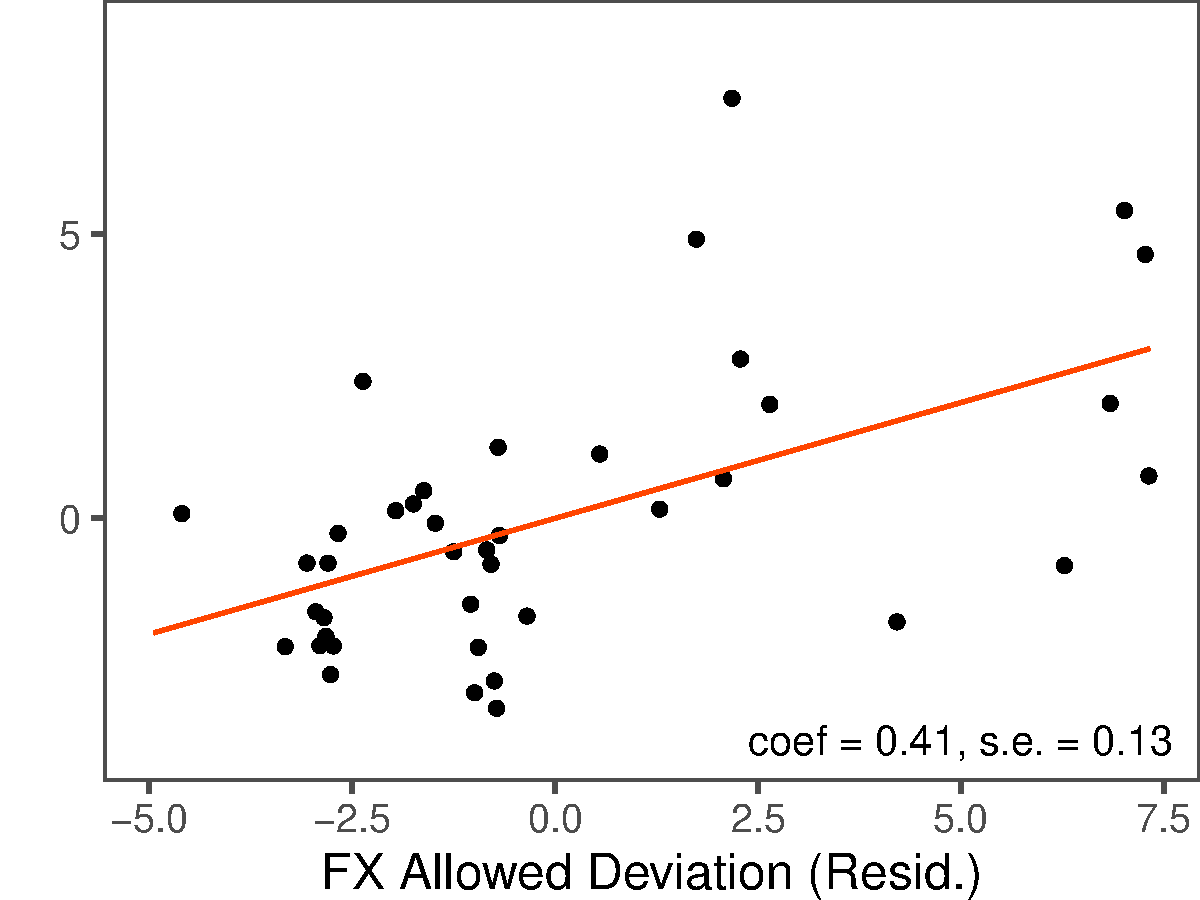
\includegraphics[width=\textwidth]{./Figures/Figure_FP_ERA.pdf}
    \end{subfigure}
    \begin{subfigure}{.33\textwidth}
      \centering
      \caption{Currency Excess Returns (Resid.)}
      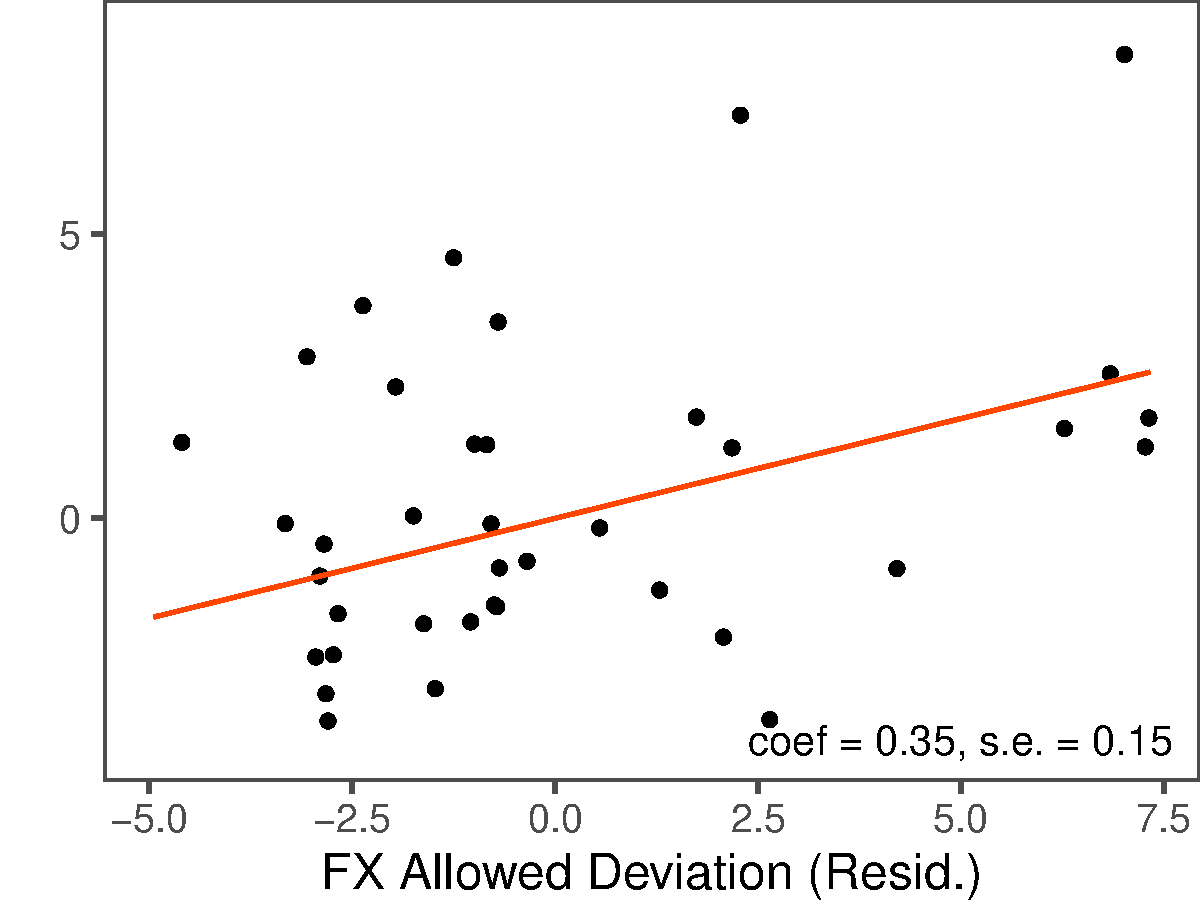
\includegraphics[width=\textwidth]{./Figures/Figure_RX_ERA.pdf}
    \end{subfigure}
    \begin{subfigure}{.33\textwidth}
      \centering
      \caption{Capital Intensity (Resid.)}
      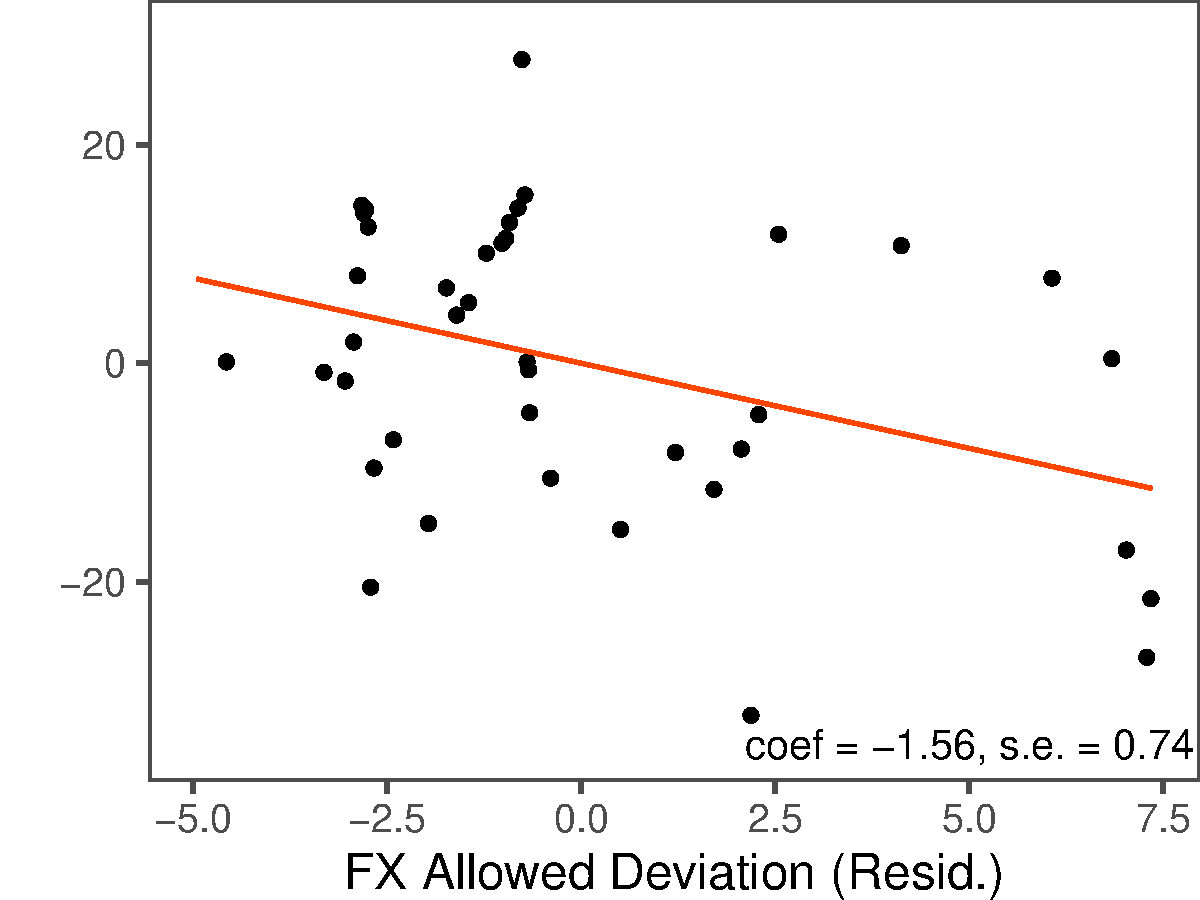
\includegraphics[width=\textwidth]{./Figures/Figure_KY_ERA.pdf}
    \end{subfigure}

    \bigskip \small \textit{Notes:} This figure shows binned
    scatterplots of the conditional relationship between each
    currency's maximum allowable annual exchange rate deviation relative to
    its target currency according to \cite{ilzetzki2018exchange} and
    (a) its ``risk-free'' interest rate differential against the US
    dollar, (b) the excess returns on the currency (that is, the
    returns measured in US dollars obtained when borrowing in dollars
    and lending in the currency in question), and (c) the capital
    intensity of production in the country issuing the currency (measured by its log
    capital to output ratio). For each panel, we regress both the
    dependent variable of interest and allowed exchange rate deviation
    on the share the country issuing the currency contributes to world
    GDP (``country size'') and show binned scatter plots of the
    residuals. The slopes shown are estimates of \(\beta\) from the
    corresponding panel regression:
    \begin{equation*}
      y_{it}
      = \alpha + \beta FX\text{ }Allowed\text{ }Deviation_{it}
      + \gamma GDP\text{ }Share_{it} + \epsilon_{it},
    \end{equation*}
    where standard errors are clusterd by currency. To derive this
    specification from our model, plug (\ref{eq_FF_UIP}) into
    (\ref{eq:stabilizationint}) and note that there is a one-for-one
    correspondence between FX Allowed Deviation and \(\zeta\). Table
    \ref{table:stylized} shows the full regression output for
    reference, including estimates of \(\gamma\) and additional
    specifications that instead us \(\zeta\) as a regressor. The
    sample consists of the intersection of the replication datasets of
    \cite{HassanMano2015} and \cite{ilzetzki2018exchange}, covering
    data for 39 currencies from 1983-2010. Panel (a) and (b) use
    monthly data; panel (c) collapses to the annual frequency. We
    assign allowed exchange rate deviations according to the fine
    exchange rate arrangement classification from
    \citet{ilzetzki2018exchange}: Codes 1, 2 and 4 are assigned 0\%
    allowed deviation; codes 5 and 7 are assigned 1\%; codes 3, 6, 8
    and 11 are assigned 2\%; codes 9, 10 and 12 are assigned 5\% and
    code 13 is assigned 10\% -- assuming that a freely floating
    exchange rate implies an allowable annual standard deviation of
    the exchange rate to the US dollar (or the euro) of 10\%). We
    treat the few currencies that do not target the dollar or the euro
    as also allowing 10\% (though doing so has no effect on our
    results). We drop the Taiwanese dollar (TWD), because it is not in
    the \citet{ilzetzki2018exchange} dataset, and we exclude the
    European currency unit (ECU) to avoid double counting Euro-area
    countries prior to 1999. Interest rate differentials in
    \citet{HassanMano2015} are measured using forward and spot
    exchange rates to isolate differences in ``risk-free'' interest
    rates that are unaffected by country default risk. Data on log
    capital to output ratios and GDP are from the Penn World Tables.
    GDP share is constructed as in \cite{Hassan2013} as the share of
    the issuing country's GDP in the total GDP of all countries in the
    sample: $GDP^j_t / \sum^N_{n = 1} GDP^n_t$.
  \end{minipage}
\end{sidewaysfigure}

\clearpage

\begin{table}[]
  \caption{2010 Exchange Rate Arrangements According to
    \citet*{ilzetzki2018exchange}\label{ta:RR}}
  \begin{center}
    \begin{tabular}{lccc}
      \hline \hline
      Panel A & \multicolumn{3}{c}{\textit{Exchange rate arrangement}} \\
      \midrule
      GDP Decile & $\quad 1 - 5 \quad$  & $\quad 6 - 9 \quad$ & $10$ \\
              &(smallest)&&(largest)\\
      \midrule
      Floating & 0\% & 0\% & 29\%\\
      Stabilized & 100\% & 100\% & 71\% \\
      \phantom{of which }soft peg & 40\% & 60\% & 65\%\\
      \phantom{of which }hard peg & 60\% & 40\% & 6\%\\
      \midrule
      Panel B & \multicolumn{3}{c}{\textit{Target currency}} \\
      \midrule
              & Dollar & Euro & Other \\
      Number of Countries          & 124   & 39 & 11 \\
      \hline \hline
    \end{tabular}
  \end{center}
  \small\textit{Notes: }Countries are divided into deciles by GDP in
  2010. Deciles 1-9 each contain 18 countries, the tenth 17 countries.
  The ``floating'' category refers to exchange rates classified as
  ``freely floating'' in \citet*{ilzetzki2018exchange} (fine
  classification code 13), the ``soft peg'' category includes
  currencies with any form of crawling peg, crawling band, or managed
  float. The ``hard peg'' category includes currency unions,
  pre-announced pegs, and de facto pegs (codes 1, 2, and 4).
\end{table}


\clearpage

\begin{figure}[!ht]
  \begin{minipage}{\linewidth}
    \begin{centering}
      \caption{Effect of Stabilization on Utility in the Stabilizing
        Country}\label{fig_welfare}
      \begin{subfigure}{.6\textwidth}
        \caption{Drivers of utility gains/losses over the size of the
          target country}
        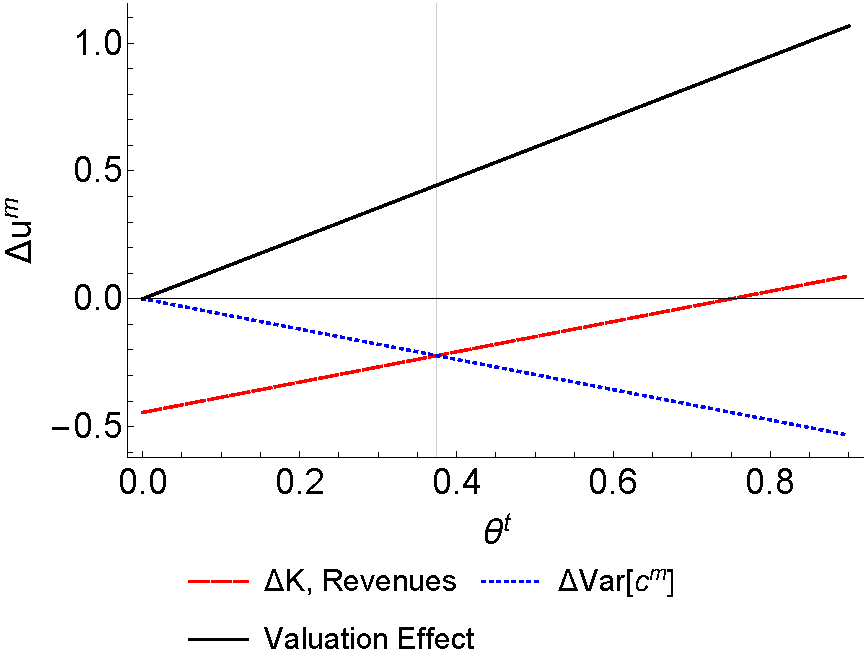
\includegraphics[width=\textwidth]{./Figures/Figure_Welfare_TgtSize.pdf}
      \end{subfigure}

      \bigskip


      \begin{subfigure}{.6\textwidth}
        \caption{{Utility gains of stabilization over strength of
            stabilization for stabilizing countries of different
            sizes}}
        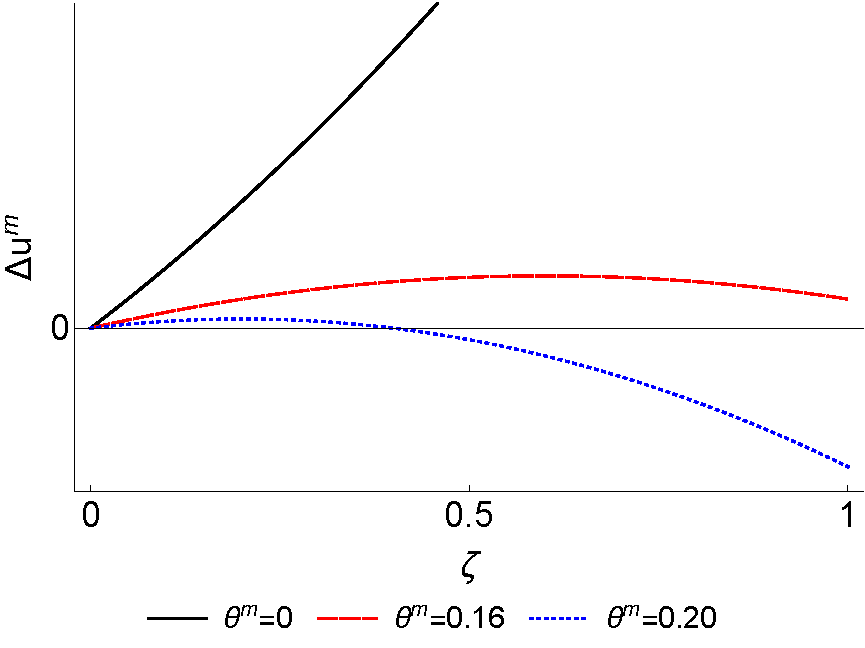
\includegraphics[width=\textwidth]{./Figures/Figure_Welfare_ThreeSizes.pdf}
      \end{subfigure}

\end{centering}
\bigskip

\small \textit{Notes:} Both plots show the percentage increase in the
certainty-equivalent consumption of a representative household in the
stabilizing country attributable to the stabilization ($\Delta u^m $)
for a numerical example where \(\tau=1/3\), and \(\gamma=7\). Panel
(a) shows the three components of $\Delta u^m $ shown on the right
hand side of (\ref{eq:Deltau}) for a small stabilizing country
($\theta^m=0$) and a hard peg (\(\zeta=1\)). The net utility gain is
the sum of the three lines. It is positive for all
\(\theta^t>\bar{\theta}\). Panel (b) shows the net utility gain as a
function of \(\zeta\) for stabilizing countries of different sizes.
See Appendix \ref{Appendix_Welfare} for the generalization of
(\ref{eq:Deltau}) that allows for $\theta^m>0$. \end{minipage}
\end{figure}

\clearpage

\begin{sidewaysfigure}[!h]
  \begin{minipage}{\linewidth}
    \begin{centering}
      \caption{Optimal Stabilizations}\label{fig_optimal}
      \begin{subfigure}{.49\textwidth}
        \caption{Optimal Choice of Exchange Rate Regime}
        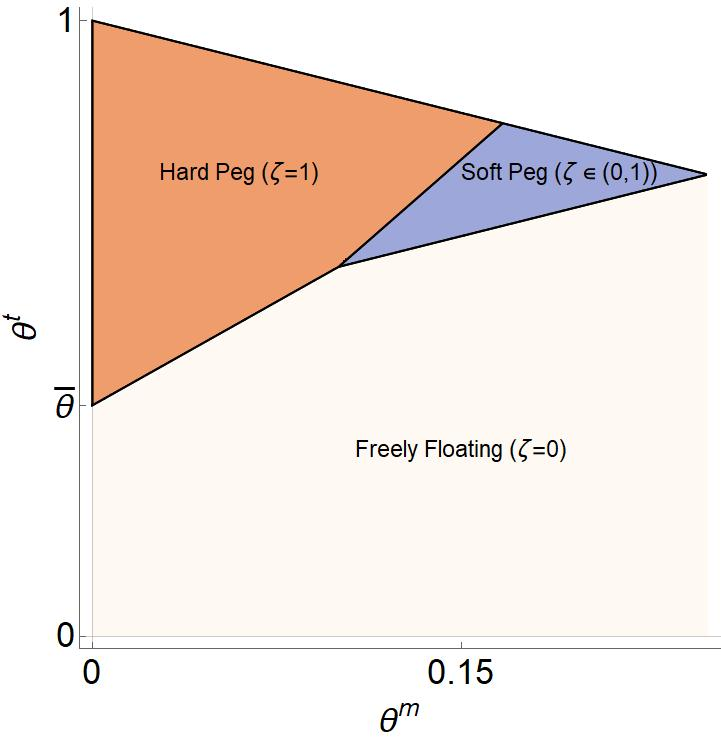
\includegraphics[width=\textwidth]{./Figures/Figure_Optimal_Policy_1.jpg}
      \end{subfigure}
      \begin{subfigure}{.49\textwidth}
        \caption{Externalities on Target and Outside Countries}
        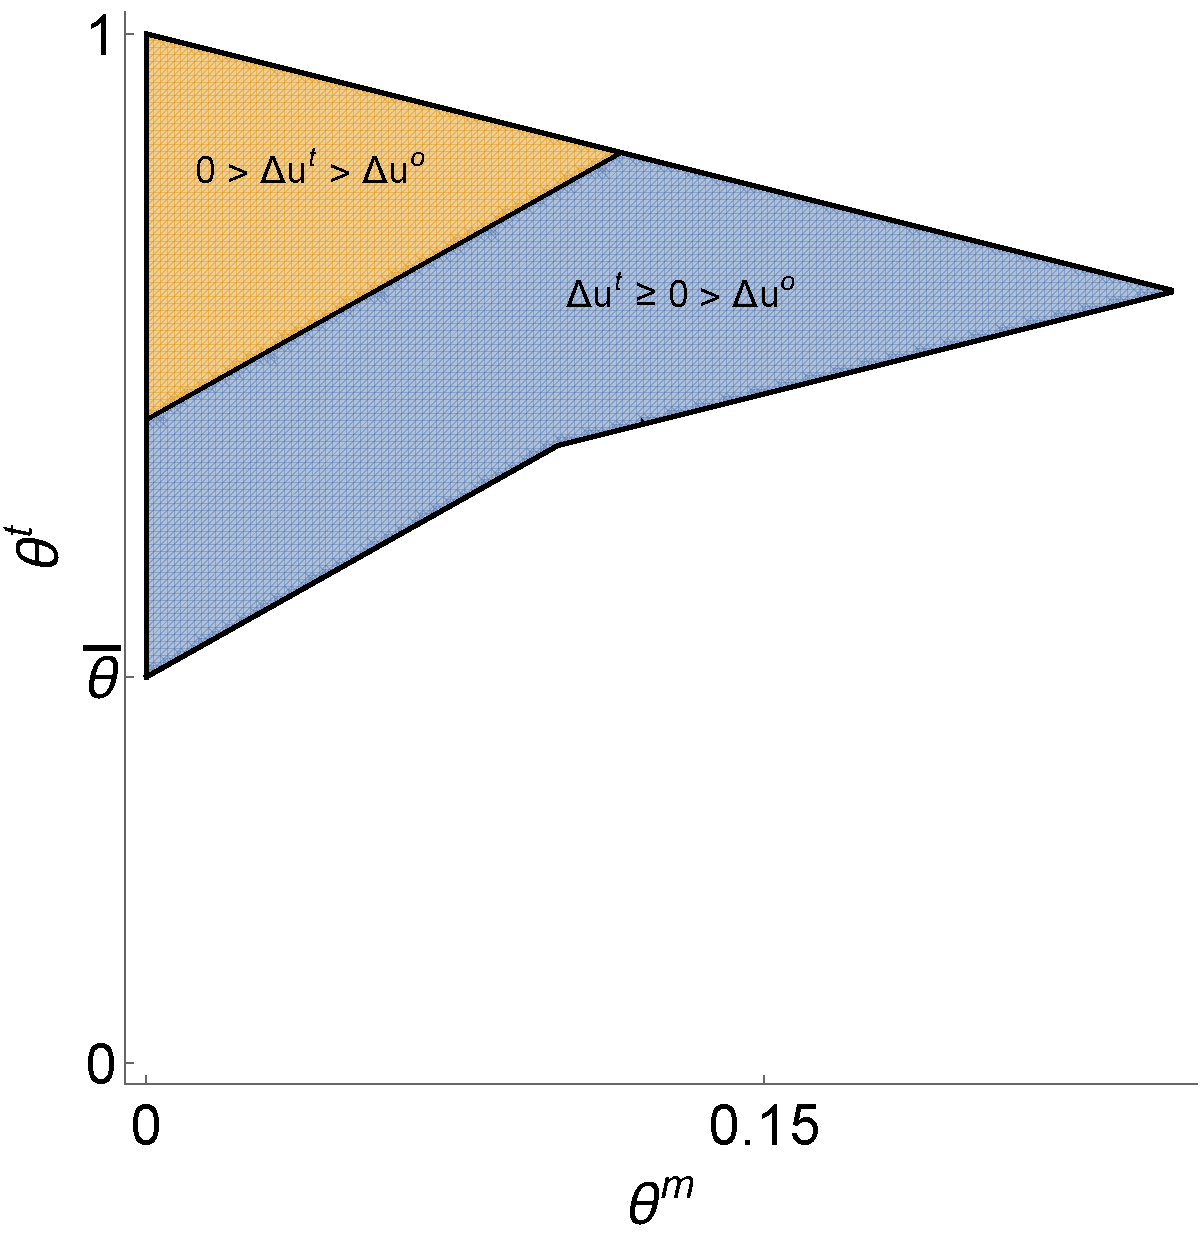
\includegraphics[width=\textwidth]{./Figures/Figure_Winners_and_Losers.pdf}
      \end{subfigure}

    \end{centering}

    \bigskip \small \textit{Notes:} The triangular region shown in
    both figures marks the subset of the parameter space where a
    stabilization is strictly welfare-increasing for the stabilizing
    country ($\Delta u^m>0 $) for a numerical example where
    \(\tau=1/3\), and \(\gamma=7\). Outside of triangular region the
    stabilizing country maximizes its own utility by floating
    ($\zeta=0 $). Panel (a) marks regions where the stabilizing
    country's optimal choice is to impose a hard peg ($\zeta=1 $,
    marked in red) versus a ``softer'' stabilization
    ($\zeta\in (0,1) $, marked in purple). Panel (b) illustrates the
    (pecuniary) externalities of these optimal stabilizations on the
    target and outside countries. \end{minipage}
\end{sidewaysfigure}

\clearpage



\bigskip \pagebreak \appendix

\FloatBarrier

\begin{center}
  {\Huge\bf Appendix}\\
  {\large\bf -For online publication only-}
\end{center}

\section{Additional Empirical Results \label{Appendix_Empirics}}

\begin{table}[htp!]
  \caption{Interest Rate Differentials, Capital Intensity, and
    Exchange Rate Regimes \vspace{-1em}}
  \label{table:stylized}
  \begin{center}
    \begin{tabular}{l c c c }
      \hline
      \hline
      Panel A: & \multicolumn{3}{c}{\emph{Table Corresponding to Figure \ref{fig_stylized}}} \\
      \cline{2 - 4} \vspace{-1em} \\
               & Interest Rate Diff. & FX Excess Returns & Capital Intensity \\
      \hline
      FX Allowed Deviation            & $0.41^{***}$   & $0.35^{**}$   & $-1.56^{**}$     \\
               & $(0.13)$       & $(0.15)$      & $(0.74)$       \\
      GDP Share & $-23.36^{***}$ & $-12.50^{**}$ & $86.82^{***}$ \\
               & $(7.54)$       & $(5.85)$      & $(27.83)$       \\
      \hline
      Num. obs.               & 7,515           & 7,515          & 662            \\
      R$^2$       & 0.12           & 0.00          & 0.06           \\
      \hline
      Panel B: & \multicolumn{3}{c}{\emph{Table with Alternative Measure of Stabilization}} \\
      \cline{2 - 4} \vspace{-1em} \\
               & Interest Rate Diff. & FX Excess Returns & Capital Intensity \\
      \hline
      $\zeta$ & $-4.08^{***}$  & $-3.51^{**}$  & $15.58^{**}$    \\
               & $(1.28)$       & $(1.49)$      & $(7.41)$       \\
      GDP Share & $-23.36^{***}$ & $-12.50^{**}$ & $86.82^{***}$ \\
               & $(7.54)$       & $(5.85)$      & $(27.83)$       \\
      \hline
      Num. obs.               & 7,515           & 7,515          & 662            \\
      R$^2$       & 0.12           & 0.00          & 0.06           \\
      \hline
      Panel C: & \multicolumn{3}{c}{\emph{Summary Statistics}} \\
      \cline{2 - 4} \vspace{-1em} \\ 
               & & Mean & Std. Dev \\
      \hline
      Interest Rate Diff. (\%) &  & 1.95 & 4.56 \\ 
      FX Excess Returns (\%) &  & 2.29 & 36.44  \\ 
      Capital Intensity (\%) & & 118.86 & 24.12 \\ 
      FX Allowed Deviation (\%) & & 3.54 & 3.65 \\ 
      $\zeta$ & & 0.65 & 0.37 \\ 
      GDP Share & & 0.04 & 0.07  \\ 
      \hline
      \hline
    \end{tabular}
  \end{center}
  \small\textit{Notes: } This table shows panel regressions of
  interest rate differentials, currency excess returns, and capital
  intensity on the allowed annual standard deviation under the issuing
  country's exchange rate regime and country size (the share the
  issuing country contributes to World GDP). The sample and data
  construction correspond to Figure \ref{fig_stylized}. Panel A shows
  the full regression output corresponding to the conditional scatter
  plots in Figure \ref{fig_stylized}. Panel B shows an alternative
  specification that follows more closely the model by using
  $\zeta=1-(FX\text{}Allowed\text{ }Deviation)/10 $ as a regressor,
  where we again assume that a freely floating exchange rate amounts
  to an allowed annual standard deviation of 10\%. Standard errors are
  clustered by currency. Panel C displays summary statistics. Capital
  intensity is the log capital to output ratio. Interest Rate Diff.,
  FX Excess Returns, Capital Intensity, and FX Allowed Deviation are
  all given in percent. See the caption of Figure \ref{fig_stylized}
  for details.
\end{table}


\clearpage

\section{Appendix to Section \ref{sec_ReducedFormResults}
  \label{Appendix_ReducedFormResults}}

The country $n$ risk-free bond pays off $P^n$ units of the traded good
at maturity. We derive the value of the risk-free bond, $V^n_P$, by
applying the asset pricing equation to the bond payoff:
\begin{equation*}
  V^n_P = \mathbb{E}\left[\Lambda_{T} P^n
  \right],
\end{equation*}
where $\Lambda_{T}$ denotes the stochastic discount factor. The
country $n$ risk-free rate (in levels), $R^n$, is the inverse of the
price of the risk-free bond:
\begin{equation*}
  R^n = \frac{1}{V^n_P}.
\end{equation*}
Putting the previous two equations together yields the following
relationship:
\begin{equation*}
  \mathbb{E}\left[ \Lambda_{T} P^n \right] R^n = 1.
\end{equation*}
As a result, the risk-free rates of countries $f$ and $h$ are related
as follows:
\begin{equation*}
  \mathbb{E}\left[\Lambda_{T} P^f \right] R^f
  = \mathbb{E}\left[\Lambda_{T} P^h \right] R^h = 1
\end{equation*} 
If the stochastic discount factor and prices are log-normal, we can
perform the following calculations:
\begin{align*}
  & \mathbb{E}\left[\Lambda_{T} P^f \right] R^f
    = \mathbb{E}\left[\Lambda_{T} P^h \right] R^h \\
  \Leftrightarrow\quad
  & \mathbb{E}\left[\exp\left[ \lambda_{T} + p^f + r^f \right]\right]
    = \mathbb{E}\left[\exp\left[\lambda_{T} + p^h + r^h \right]\right] \\
  \Leftrightarrow\quad
  & \mathbb{E}\left[\lambda_{T} + p^f\right] + \frac{1}{2}\text{var}\left(\lambda_{T}\right) + 
    \frac{1}{2}\text{var}\left(p^f\right) + \text{cov}\left(\lambda_{T}, p^f\right) + r^f \\
  & = 
    \mathbb{E}\left[\lambda_{T}+ p^h\right] + \frac{1}{2}\text{var}\left(\lambda_{T}\right)+ 
    \frac{1}{2}\text{var}\left(p^h\right) + \text{cov}\left(\lambda_{T}, p^h\right)+r^h,
\end{align*}
We cancel out $\text{var}\left( \lambda_{T} \right)$ from both sides
of the previous equation.
\begin{align*}
  &\mathbb{E}\left[p^f\right]+\frac{1}{2}\text{var}\left(p^f\right) + \text{cov}\left(\lambda_T, p^f\right)+r^f
    = \mathbb{E}\left[p^h\right]+\frac{1}{2}\text{var}\left(p^h\right)+\text{cov}\left(\lambda_T,p^h\right)+r^h
  \\      \Leftrightarrow \quad
  & r^f+\mathbb{E}\left[p^f-p^h\right]+\frac{1}{2}\text{var}\left(p^f\right)-\frac{1}{2}\text{var}\left(p^h\right)-r^h = -\text{cov}\left(\lambda_T,p^f-p^h\right)\\   
  \Leftrightarrow\quad
  &r^f+\log\left(\mathbb{E}\left[P^f\right]/\mathbb{E}\left[P^h\right]\right)-r^h = -\text{cov}\left(\lambda_T,p^f-p^h\right)
\end{align*}
We define
$\Delta\mathbb{E}\left[s^{f,h}\right]
=\log\left(\mathbb{E}\left[P^f\right]/\mathbb{E}\left[P^h\right]\right).$
With this definition:
\begin{equation*}
  r^f+\Delta\mathbb{E}\left[s^{f,h}\right]-r^h = -\text{cov}\left(\lambda_T,p^f-p^h\right).
\end{equation*}


\section{Appendix to Sections \ref{sec:environment} -
\ref{sec:positive_effects}}


\subsection{Equilibrium Conditions
  \label{Appendix_ModelDetails}}

In this appendix, we provide additional details for our baseline model
in Section \ref{sec:environment} and formally derive its equilibrium
conditions. To avoid solving the optimization problem separately for
households in the stabilizing country and households in the rest of
the world, we generalize the notation to allow all countries to impose
state-contingent taxes, $Z^n(\omega)$, and provide lump sum transfers,
$\bar{Z}^n$. The governments in the target and outside countries do
not use these instruments, such that $Z^t(\omega)=Z^o(\omega) = 1$ and
$\bar{Z}^t =\bar{Z}^o= 0$.

In the second period, all households maximize their utility
(\ref{eqn:utility}) subject to their budget constraint:
\begin{equation}
  Z^n(\omega) C_T^n(\omega) + P_N^n(\omega) C_N^n(\omega)  
  \le \sum_l A_l^n P_N^l(\omega) Y_N^l(\omega) + Y_T 
  \label{eqn:budget_cons_2}
\end{equation}
where $P^n_N(\omega)$ is the price of the nontraded good in the
stabilizing country in state $\omega$, $A^n_l$ is number the stocks a
country $n$ household owns in the firm in country $l$, and $Y_T = 1$
is the unit endowment of the traded good.

In the first period, households choose their portfolio of stocks to
maximize expected utility in the second period. The first-period
budget constraint reads:
\begin{equation}
  \sum_l A_l^n Q^l_N + Q_K K^n_N \le W^n_0.
  \label{eqn:budget_cons_1}
\end{equation}
where $W^n_0$ represents initial household wealth in terms of traded
goods in the first period.

$\Lambda_T^n(\omega)$ denotes the Lagrange multiplier on the budget
constraint for the country $n$ household in state $\omega$ in the
second period. The first-order conditions are:
\begin{align}
  \frac{\tau \left( C^n(\omega)^{1 - \gamma} \right) 
  \left( C_T^n(\omega) \right)^{-1}}{Z^n(\omega)}
  & = \Lambda^n_T(\omega) \label{eqn:FOCCT_full}\\ 
  (1 - \tau) \left( C^n(\omega)^{1 - \gamma} \right) 
  \left( C_N^n(\omega) \right)^{-1} & = \Lambda^n_T(\omega) P^n_N(\omega).
                                      \label{eqn:FOCCN_full}
\end{align}
The consumption tax drives a wedge between the marginal utility of
consumption of traded goods and its shadow price, as equation
\eqref{eqn:FOCCT_full} shows. Equations \eqref{eqn:FOCCN} and
\eqref{eqn:FOCCN_full} jointly imply
$P_N^n(\omega)= \Lambda_N^n(\omega) / \Lambda^n_T(\omega)$.

Next, we derive equilibrium conditions that determine first-period
investment in stocks and capital. Since the final consumption bundle
is a Cobb-Douglas aggregate of traded and nontraded goods, households
spend a fraction $\tau$ of their second-period wealth on traded
consumption and a fraction $1 - \tau$ on nontraded consumption:
\begin{align*}
  C^n_T(\omega) = \tau
  \left( \frac{\sum_l A^n_l P^l_N(\omega) Y^l_N(\omega) + 
  Y_T}{Z^n(\omega)} \right) \text{ and }
  C^n_N(\omega) = (1 - \tau)
  \left( \frac{\sum_l A^n_l P^l_N(\omega) Y^l_N(\omega) + 
  Y_T}{P^n_N(\omega)} \right).
\end{align*}
In the first period, households choose their portfolio of stocks and
firms decide on their capital investment, $K^n_N$. We plug the
consumption of traded and nontraded goods into equations
(\ref{eqn:cesutil}) and (\ref{eqn:utility}) and take first-order
conditions to obtain:
\begin{equation*}
  Q^l_N
  = \mathbb{E}\left[
    \left( \frac{\tau^\tau (1 - \tau)^{1 -\tau}}{\Lambda_{T, 1}^n \left( Z^n(\omega) \right)^{\tau}
        \left(P^n_N(\omega) \right)^{1 - \tau}} \right)
    \left( C^n(\omega) \right)^{- \gamma} P^l_N(\omega) Y^l_N(\omega) \right],
\end{equation*}
where $\Lambda_{T, 1}^n$ denotes the Lagrange multiplier on the
first-period budget constraint for a household in country $n$.


Divide through by $Q^l_N$ and apply the definition of the price index
$P^n(\omega)$ given by equation \eqref{eqn:price_index} in Appendix
\ref{Appendix_PriceIndex} to obtain
\begin{equation}
  \mathbb{E}\left[ \frac{\Lambda_T^n(\omega)}{\Lambda_{T, 1}^n} 
    \frac{P^l_N(\omega) Y^l_N(\omega)}{Q_N^l} \right] = 1.
  \label{eqn:FOC_Stock}
\end{equation}

Firms invest in capital to maximize the expected discounted value of
profits:
\begin{equation*}
  \max_{K^n} \mathbb{E}\left[ 
    \left( \frac{\Lambda^n_T(\omega)}{\Lambda^n_{T, 1}} \right) 
    P_N^n(\omega) \exp\left( \eta^n \right) \left( K^n \right)^{\nu} \right] - 
  Q_K \left( K^n - 1 \right).
\end{equation*}
Their first-order condition with respect to $K^n$
yields\begin{equation*} Q_K = \nu \mathbb{E}\left[
    \frac{\Lambda_T^n(\omega)}{\Lambda_{T, 1}^n} P^n_N(\omega)
    \exp\left( \eta^n \right) \left(K^n\right)^{\nu - 1} \right].
\end{equation*}
Multiply both sides of the previous equation by $K^n$, divide by
$Q_K$, substitute $Y_N^n = \exp(\eta^n) \left( K^n \right)^\nu$, and
apply the definition of $P^n_N(\omega)$ to get (\ref{eqn:FOCK}).

Equations \eqref{eqn:FOC_Stock} and \eqref{eqn:FOCK} show
$\Lambda^n_T(\omega) / \Lambda^n_{T, 1}$ are the stochastic discount
factors used to price assets that pay off in traded goods in the
second period. Since stocks and capital are freely traded in
international markets, all households must be marginal to investing in
all stocks and all firms must be marginal to purchasing an additional
unit of capital. As a result, the stochastic discount factors are
equal in equilibrium across countries,
\begin{equation}
  \frac{\Lambda^n_T(\omega)}{\Lambda^n_{T, 1}} = 
  \frac{\Lambda^m_T(\omega)}{\Lambda^m_{T, 1}} \quad
  \forall ~n, m,
  \label{eqn:sdf_equal}
\end{equation}
even though the government's intervention drives a wedge between
$\Lambda_T(\omega)$ and the marginal utility of traded consumption in
the stabilizing country, as equation \eqref{eqn:FOCCT_full} shows.

As a final step, we derive the equations that pin down the first and
second-period Lagrange multipliers. Household wealth in the first
period is:
\begin{equation*}
  W^n_0 = Q^n_N + Q_K + \kappa^n + \bar{Z}^n,
\end{equation*}
Recall that households are endowed with a unit of stock and a unit of
capital. $\kappa^n$ is the transfer that equalizes the marginal
utility of wealth across households when countries do not manipulate
the exchange rate, and the transfer $\bar{Z}^m$ ensures the same is
true under a stabilization, so that\begin{equation} \Lambda^{n}_{T, 1}
  = \Lambda^{}_{T, 1} \quad \forall ~n.
  \label{eqn:mult_equal}
\end{equation}
As a result, \eqref{eqn:sdf_equal} implies
\begin{equation*}
  \Lambda^n_T(\omega) = \Lambda_T(\omega)
  \quad \forall ~n, \omega.
\end{equation*}

Hence, we drop the country index on the Lagrange multipliers, and
interpret $\Lambda_T(\omega)$ as the shadow price of traded
consumption in the target and outside countries in the second period.
This result implies equations \eqref{eqn:FOCCT}, \eqref{eqn:FOCCN} and
\eqref{eqn:FOCK}.

Equation \eqref{eqn:mult_equal} shows the first-period Lagrange
multipliers are equal to each other, but it does not determine the
level of the Lagrange multipliers. Without loss of generality, we
normalize the first period Lagrange multiplier:
\begin{equation}
  \Lambda_{T, 1} =  \mathbb{E}\left[ \Lambda^n_T(\omega) \right].
  \label{eqn:norm_lambda}
\end{equation}


\subsection{Deriving the Price Index \label{Appendix_PriceIndex}}
The cost of one unit of consumption in country $n$ is given by the price index
\begin{equation}
  P^n = \arg \min C_T^n + P_N^n C_N^n \text{ s.t. } 
  \left( C_T^n \right)^\tau \left( C_N^n \right)^{1 - \tau} = 1.
  \label{eqn:InactiveProblem}
\end{equation}
First-order conditions imply
$C^n_N = \left( 1 - \tau \right) / \left( P^n_N \tau \right) C^n_T$. We plug
this expression for $C_N^n$ into the constraint
$\left( C_T^n \right)^\tau \left( C_N^n \right)^{1 - \tau} = 1$, and
solve for $C_T^n$:
\begin{equation*}
  C_T^n = \left( \frac{\tau}{1 - \tau} P_N^n \right)^{1 - \tau}.
\end{equation*}
We plug the expressions for $C_T^n$ and $C_N^n$ back into equation
(\ref{eqn:InactiveProblem}) to derive the optimal price index:
\begin{equation}
  P^n = \frac{ \left( P_N^n \right)^{1 - \tau}}{\tau^\tau (1 - \tau)^{1 - \tau}}.
  \label{eqn:price_index}
\end{equation}
The total value of consumption for households in country $n$ is
\begin{equation*}
  P^n C^n = 
  \left( \frac{ \left( P_N^n \right)^{1 - \tau}}{\tau^\tau (1 - \tau)^{1 - \tau}} \right)
  \left( \left( C_T^n \right)^\tau \left( C_N^n \right)^{1 - \tau} \right) = 
  \frac{C_T^n}{\tau}.
\end{equation*}
Similarly, we use the expression
$P_N^n = \frac{1 - \tau}{\tau}\frac{C_T^n}{C_N^n}$ to show that
\begin{equation*}
  C_T^n + P_N^n C_N^n = \frac{C_T^n}{\tau} = P^n C^n.
\end{equation*}

\subsection{Log-linearized System of
  Equations \label{Appendix_Loglinear}}

This appendix derives the log-linearized first-order conditions. To
reiterate, we log-linearize around the deterministic solution --- the
point at which the variances of shocks are zero
$\left( \sigma_{N, n} = 0 \right)$ and all firms have a capital stock
fixed at the deterministic steady-state level.

We have shown in Appendix \ref{Appendix_ModelDetails} that the
stochastic discount factor $\Lambda^n_T(\omega) / \Lambda^n_{T, 1}$ is
equalized across all households in all states. It is convenient to
write the logarithm of this stochastic discount factor as:
\begin{equation*}
  q = \lambda^n_T - \lambda^n_{T, 1}.
\end{equation*}
We can then write the log-linear first-order conditions for the second
period as
\begin{align*} (1 - \gamma) \left( \tau c_T^n + (1 - \tau) c_N^n
  \right) - c_T^n + \log \tau
  & = z^n  + q + \lambda^n_{T, 1} \\
  (1 - \gamma) \left( \tau c_T^n + (1 - \tau) c_N^n \right) - c_N^n +
  \log(1 - \tau) &= p_N^n + q + \lambda^n_{T, 1},
\end{align*}
and the log-linear resource constraints are:
\begin{align*}
  c_N^n & =  y_N^n \\
  \sum_{n = m, t, o} \theta^n c_T^n  & = 0 
\end{align*}
where $z^m = \log \left( Z^m(\omega) \right)$ and \(z^t=z^o=0\). Note
that $\Delta Res$ is a second-order term (linear in $\sigma^n$) and
consequently does not show up in the log-linear resource constraint.
This set of ten linear equations (two first order conditions for each
country and four resource constraints) allows us to solve for the
endogenous variables
$\left\{c_N^n, c_T^n, p_N^n \right\}_{n = m, t, o}$ and $q$. Keeping
in mind the log-linear relationship between each country's output and
its respective productivity shock (\ref{eqn:prodN}), it is convenient
to solve for these endogenous variables in terms of each country's
output $\left\{ y_N^m, y_N^t, y_N^o\right\}$, and the Lagrange
multipliers
$\left\{\lambda_{T, 1}^m, \lambda_{T, 1}^t, \lambda_{T, 1}^o
\right\}$.

Solving the system yields:
\begin{align*}
  c_T^m
  & = \frac{(\gamma - 1)(1 - \tau)}{1 + (\gamma - 1) \tau} \left( \bar{y}_N - y_N^m \right)
    - \frac{1 - \theta^m}{1 + (\gamma - 1) \tau} z^m
    + \frac{\bar{\lambda}_{T, 1} - \lambda^m_{T, 1}}{1 + (\gamma - 1) \tau} \\
  c_T^t
  & = \frac{(\gamma - 1)(1 - \tau)}{1 + (\gamma - 1) \tau} \left( \bar{y}_N - y_N^t \right)
    + \frac{\theta^m}{1 + (\gamma - 1) \tau} z^{m}
    + \frac{\bar{\lambda}_{T, 1} - \lambda^t_{T, 1}}{1 + (\gamma - 1) \tau}  \\
  c_T^o
  & = \frac{(\gamma - 1)(1 - \tau)}{1 + (\gamma - 1) \tau} \left( \bar{y}_N - y_N^o \right)
    + \frac{\theta^m}{1 + (\gamma - 1) \tau} z^{m}
    + \frac{\bar{\lambda}_{T, 1} - \lambda^o_{T, 1}}{1 + (\gamma - 1) \tau} \\
  c_N^n
  & = y_N^n \quad \forall n
\end{align*}
where $\bar{\lambda}_{T, 1} = \sum_n \theta^n \lambda^n_{T, 1}$. In
addition, we have the equilibrium prices:
\begin{align*}
  q
  & = - (1 - \tau)(\gamma - 1) \bar{y}_N - \theta^m z -
    \bar{\lambda}_{T, 1} \\
  p_N^m
  & = \frac{(\gamma - 1)(1 - \tau)}{1 + (\gamma - 1) \tau}
    \bar{y}_N - \frac{\gamma}{1 + (\gamma - 1) \tau} y_N^m +
    \frac{\theta^m + (\gamma - 1) \tau}{1 + (\gamma - 1) \tau}
    z^{m} + \frac{\bar{\lambda}_{T, 1} - \lambda^m_{T, 1}}{1 +
    (\gamma - 1) \tau}
    + \log [\frac{1 - \tau}{\tau}] \\
  p_N^t
  & = \frac{(\gamma - 1)(1 - \tau)}{1 + (\gamma - 1) \tau}
    \bar{y}_N - \frac{\gamma}{1 + (\gamma - 1) \tau} y_N^t +
    \frac{\theta^m}{1 + (\gamma - 1) \tau} z^{m} +
    \frac{\bar{\lambda}_{T, 1} - \lambda^t_{T, 1}}{1 + (\gamma -
    1) \tau}
    + \log [\frac{1 - \tau}{\tau}] \\
  p_N^o
  & = \frac{(\gamma - 1)(1 - \tau)}{1 + (\gamma - 1) \tau}
    \bar{y}_N - \frac{\gamma}{1 + (\gamma - 1) \tau} y_N^o +
    \frac{\theta^m}{1 + (\gamma - 1) \tau} z^{m} +
    \frac{\bar{\lambda}_{T, 1} - \lambda^o_{T, 1}}{1 + (\gamma -
    1) \tau} + \log [\frac{1 - \tau}{\tau}]
\end{align*}
It is also useful to keep track of the shadow prices of total
consumption in each country. To this end, we also use the log-linear
expression
$\lambda^n = -\gamma \left( \tau c_T^n + (1 - \tau) c_N^n \right)$
along with the solutions for traded and nontraded consumption above to
obtain:
\begin{align*}
  \lambda^m & = - \frac{(\gamma - 1)(1 - \tau) \gamma \tau}{1 + (\gamma - 1) \tau} \overline{y}_N
              - \frac{\gamma (1 - \tau)}{1 + (\gamma - 1) \tau} y_N^m
              + \frac{\left( 1 - \theta^m \right) \gamma \tau}{1 + (\gamma - 1) \tau} z^{m}
              - \frac{\gamma \tau \left( \bar{\lambda}_{T, 1} - \lambda^m_{T, 1} \right)}{1 + (\gamma - 1) \tau}\\
  \lambda^t & = - \frac{(\gamma - 1)(1 - \tau) \gamma \tau}{1 + (\gamma - 1) \tau} \overline{y}_N
              - \frac{\gamma (1 - \tau)}{1 + (\gamma - 1) \tau} y_N^t
              + \frac{\theta^m \gamma \tau}{1 + (\gamma - 1) \tau} z^{m}
              - \frac{\gamma \tau \left( \bar{\lambda}_{T, 1} - \lambda^t_{T, 1} \right)}{1 + (\gamma - 1) \tau}  \\
  \lambda^o & = - \frac{(\gamma - 1)(1 - \tau) \gamma \tau}{1 + (\gamma - 1) \tau} \overline{y}_N
              - \frac{\gamma (1 - \tau)}{1 + (\gamma - 1) \tau} y_N^o + 
              \frac{\theta^m \gamma \tau}{1 + (\gamma - 1) \tau} z^{m}
              - \frac{\gamma \tau \left( \bar{\lambda}_{T, 1} - \lambda^o_{T, 1} \right)}{1 + (\gamma - 1) \tau} 
\end{align*}

Finally, the following log-linear equations determine the first-period
Lagrange multipliers. Again, recall the stabilizing country's
government uses $\bar{Z}^m$ to add and subtract resources from the
economy to achieve (P2), which equalizes the marginal utility of
initial wealth across households. As a result:
\begin{equation*}
  \lambda^m_{T, 1} = \lambda^t_{T, 1} = \lambda^o_{T, 1} = \lambda_{T, 1},
\end{equation*}
so that the remaining endogenous term drop out of the solutions above,
\(\bar{\lambda}_{T, 1} - \lambda^m_{T, 1}=0\). Next, we normalize
$\lambda_{T, 1}$ using the second-order approximation of equation
\eqref{eqn:norm_lambda}:
\begin{equation*}
  \lambda_{T, 1}
  = \mathbb{E} \left[ \lambda_{T} \right]
  + \frac{1}{2} var\left[ \lambda_{T} \right].
\end{equation*}

\subsection{Equilibrium Asset Portfolio
  \label{Appendix_Decentralization}}

In the log-linear solution, all prices and quantities are a linear
combination of $\left\{ y_N^m, y_N^t, y_N^o\right\}$. In particular, household
expenditure, $p^n + c^n$, in each state of the world is a linear
combination of $\left\{ y_N^m, y_N^t, y_N^o\right\}$. All asset payoffs are also
linear combinations of $\left\{ y_N^m, y_N^t, y_N^o\right\}$. Any set of assets with
the same rank as the set of household expenditures will thus be able to span the
space of household expenditure. Therefore, given the appropriate set of
assets, we can write household expenditure in each state of the world as a
linear combination of these assets.

It is straightforward to verify that the set of log-linear stock
payoffs spans the space of log-linear household wealth.
\begin{lemma}
  Households in the freely floating exchange rate equilibrium hold
  levered positions in their own country's stocks and hold short
  positions in other countries' stocks,
  \begin{equation*}
    A_n^n = \frac{1 - \theta^n \tau}{1 - \tau} \text{ and }
    A_l^n = - \frac{\theta^n \tau}{1 - \tau} \text{ for } l \neq n
  \end{equation*}
  \label{Lemma_AssetPortfolio}
\end{lemma}
\begin{proof}
  The household budget constraint \eqref{eqn:budget_cons_2} can be
  re-written as:
  \begin{equation*}
    P^n(\omega) C^n(\omega)
    = \sum_{l = m, t, o} A_l^n P^n_N(\omega) Y^n_N(\omega) + Y^n_T
  \end{equation*}
  The log-linear approximation of household expenditure of the
  left-hand side is:
  \begin{equation*}
    \frac{1}{\tau} \left( p^n + c^n + \log \left[ \tau \right] \right)
    = \frac{(\gamma - 1)(1 - \tau)}{\tau \left( 1 - (\gamma - 1) \tau \right)}
    \left( \bar{y}_N - y^n_N \right) 
  \end{equation*}
  The log-linear approximation the stock portfolio payoff (right-hand
  side) is:
  \begin{equation*}
    \sum_{l = m, t, o} A_l^n \frac{1 - \tau}{\tau}
    \left( p^{l \ast}_N + y^l_N - \log\left[ \frac{1 - \tau}{\tau} \right] \right).
  \end{equation*}
  where:
  \begin{equation*}
    p^{l \ast}_N + y^l_N
    = \frac{(\gamma - 1)(1 - \tau)}{1 + (\gamma - 1) \tau }
    \left( \bar{y}_N - y^l_N \right) 
    + \log\left[ \frac{1 - \tau}{\tau} \right].
  \end{equation*}
  We equate household expenditures in each state of the world with the
  portfolio payoff:
  \begin{equation*}
    \frac{(\gamma - 1)(1 - \tau)}{\left( 1 - (\gamma - 1) \tau \right)}
    \left( \bar{y}_N - y^n_N \right) 
    = \sum_{l = m, t, o} A_l^n \frac{1 - \tau}{\tau}
    \left( p^{l \ast}_N + y^l_N - \log\left[ \frac{1 - \tau}{\tau} \right] \right)
  \end{equation*}
  Since this equation holds state-by-state, we solve for the shares,
  $A^n_l$, by matching the coefficients on $y^l_N$ in the portfolio
  payoff with the coefficients on $y^l_N$ in household expenditure.
\end{proof}


\subsection{Derivation of Equation
  \eqref{eq_link_k_r} \label{app_cap}}

To derive (\ref{eq_link_k_r}), we use the following second-order
approximation of equation (\ref{eqn:FOCK}):
\begin{equation*}
  \lambda_{T, 1} + q_K + k^n
  = \log[\nu] + \mathbb{E}\left[ \lambda_N^n + y_N^n \right]
  + \frac{1}{2} \text{var}\left( \lambda_N^n + y_N^n \right),
\end{equation*}
%$k^n = 0$, $\mathbb{E}[y_N^n] = -\frac{1}{2} \sigma^2_N$ , and $\text{var}[y_N^n] = \sigma_N^2$.
Next, we substitute
$\lambda^{n}_{N}=p^{n}_{N}+ \lambda_T$, and take differences across
two arbitrary countries $f$ and $h$ to obtain:
\begin{equation}
  k^f - k^h
  = \frac{1}{2} \text{var}\left( p_{N}^f + y_{N}^f \right)
  - \frac{1}{2} \text{var}\left( p_{N}^h + y_{N}^h \right)
  + \text{cov}\left( p_{N}^f + y_{N}^f - p_{N}^h - y_{N}^h, \lambda_{T}\right).
  \label{eqn:kspread} 
\end{equation}
For any country $n$:
\begin{equation*}
  p_{N}^{n*}  + y_{N}^{n*} = 
  \frac{(1 - \tau)(\gamma - 1)}{1 + (\gamma - 1) \tau}
  \left( \bar{y}_{N} - y_{N}^n \right).
\end{equation*}
Plugging this expression for $p_{N}^{n*} + y_{N}^{n*}$ into the
right-hand side of equation (\ref{eqn:kspread}) shows:
\begin{equation*}
  k^{f*} - k^{h*} = 
  \frac{(\gamma - 1)^3 (1 - \tau)^2 \tau}{1 + (\gamma - 1) \tau}
  \left( \theta^f - \theta^h \right)\sigma_N^2. 
\end{equation*}
Combine this equation with equation (\ref{eq_FF_UIP}) to derive
(\ref{eq_link_k_r}),

\subsection{Proof of Lemma
  \ref{lemma:CostofPeg}
  \label{Appendix_ProofCostofPeg}}

First, we solve for the state-contingent taxes that implement the real
exchange rate stabilization. Afterwards, we derive an expression for
the cost of stabilizing the exchange rate. We guess a tax of the form
$Z(\omega) = \left( Y_N^m(\omega) / Y_N^t(\omega) \right)^a$
stabilizes the exchange rate for a constant $a$ and solve for the
coefficient $a$ that stabilizes the real exchange rate. In logs, this
tax is: $z = a \left( y_N^t - y_N^m \right)$. We plug this expression
into the solution of the model derived in Appendix
\ref{Appendix_Loglinear} and solve for the log real exchange rate:
\begin{equation*}
  s^{m, t} = 
  \frac{\gamma (1 - \tau)}{1 + (\gamma - 1) \tau} \left( y_N^t - y_N^m \right) 
  + a \frac{\gamma \tau}{1 + (\gamma - 1) \tau} \left( y_N^m - y_N^t \right). 
\end{equation*}
Choose $a$ such that $s^{m, t} = (1 - \zeta) s^{m, t \ast}$. This
yields $a = \zeta (1 - \tau) / \tau$. Finally, we use the expression
for $s^{f, h \ast}$ given by equation \eqref{eqn:rerNP} to write $z$
as a function of $p^{m \ast}$ and $p^{t \ast}$.

$\Delta Res$ is defined by equation (\ref{eqn:kappacost}). First, we
solve for $\bar{Z}$ by plugging in the equilibrium consumption of
nontraded goods and $K^m = 1$ into the budget constraint
\eqref{eqn:budget_cons_1}:
\begin{equation*}
  \bar{Z}
  = \left( A^m_m - 1 \right) Q^m_N + \sum_{l \neq m} A^m_l Q^l_N 
  - \kappa^m.
\end{equation*}
Next, multiply equation (\ref{eqn:budget_cons_2}) by the stochastic
discount factor, $\Lambda_T(\omega) / \Lambda_{T, 1}$, and take
expectations to derive the present value of tax revenues:
\begin{align*}
  &  \mathbb{E}\left[ 
    \left( \frac{\Lambda_T(\omega)}{\Lambda_{T, 1}} \right) 
    \left(Z(\omega) - 1\right) C^m_T(\omega) \right] \\
  = & \mathbb{E}\left[ 
      \left( \frac{\Lambda_T(\omega)}{\Lambda_{T, 1}} \right) 
      \left( \left( A^m_m - 1 \right) P^m_N(\omega) Y^m_N(\omega) +
      \sum_{l \neq m} A^m_l P^m_N(\omega) Y^m_N(\omega) + Y^n_T -
      C^m_T(\omega) \right) \right] \\
  = & \left( A^m_m - 1 \right) Q^m_N + \sum_{l \neq m} A^m_l Q^l_N + 
      Y^m_T \mathbb{E} \left[ \left( 
      \frac{\Lambda_T(\omega)}{\Lambda_{T, 1}} \right) \right] - 
      \mathbb{E}\left[ 
      \left( \frac{\Lambda_T(\omega)}{\Lambda_{T, 1}} \right) 
      C^m_T(\omega) \right] 
\end{align*}
Finally, we derive $\kappa^m$. In the freely floating exchange rate
economy, $\bar{Z} = 0$ and $Z(\omega) = 1$. Plug these values into
equations (\ref{eqn:budget_cons_2}) and (\ref{eqn:budget_cons_1}).
Finally, we substitute equation \eqref{eqn:norm_lambda} and use the
fact that $Y^m_T$ is a constant to show:
\begin{equation}
  \kappa^m = \mathbb{E}\left[ 
    \left( \frac{\Lambda^{\ast}_T(\omega)}{\Lambda^{\ast}_{T, 1}} \right) 
    C_T^{m \ast}(\omega) \right]  - Y^m_T 
  \label{eqn:defn_kappa}
\end{equation}
We plug the expressions for $\bar{Z}$, the present value of tax
revenues, and $\kappa^m$ in equation \eqref{eqn:kappacost}, and
simplify to arrive at equation \eqref{eq:kappacost}.

We also derive the portfolio of stocks that exactly finances the
stabilization policy. This is the portfolio that pays the difference
between traded consumption when stabilizing and traded consumption in
the freely floating regime given by equation \eqref{eqn:cTp}. For
convenience, this equation is repeated here where
$p^{t \ast} - p^{m \ast}$ is written in terms differences in nontraded
output:
\begin{equation*}
  c^m_T - c^{m \ast}_T
  = \zeta
  \frac{(1 - \theta^m)(1 - \tau)}{\tau \left( 1 + (\gamma - 1) \tau \right)}
  \left( y^t_N - y^m_N \right).
\end{equation*}
We use the same log-linear approximation of the stock portfolio as in
Appendix \ref{Appendix_Decentralization}. Letting $A^m_l$ denote the
number of shares of country $l$ stock the stabilizing country's
central bank holds, we get\begin{equation*} A^m_m = \zeta \frac{1 -
    \theta^m}{\gamma - \zeta (\gamma - 1)(1 - \tau)} \text{, } A^m_t =
  - A^m_m \text{, } A^m_o = 0.
\end{equation*}


\subsection{Proof of Proposition
  \ref{prop:KNRBCPeg} \label{Appendix_KNRBCPeg}}

We use the expressions from Appendix \ref{Appendix_Loglinear} to
calculate $p^t - p^m = \lambda^t - \lambda^m$ and we plug the
resulting expression into equation \eqref{eq_UIP_RF}:
\begin{align*}
  r^m + \Delta \mathbb{E}s^{m, t} - r^t
  &= \text{cov}\left( \lambda_T, p^t - p^m \right) \\
  &= \left(r^{m \ast} + \Delta \mathbb{E}s^{m, t \ast} - r^{t \ast} \right)
    - \zeta \frac{(1 - \tau)^2 \gamma \left( 2 \theta^m (1 - \zeta)
    + \left( \theta^t - \theta^m \right) (\gamma - 1) \tau \right)}
    {\tau \left( 1 + (\gamma - 1) \tau \right)} \sigma_N^2.
\end{align*}
When the stabilizing country is smaller than the target country,
$\theta^m < \theta^t$, the right-hand side of this expression implies
the stabilization decreases the risk-free rate in the stabilizing
country relative to the risk-free rate in the target country.

We use equation (\ref{eqn:kspread}) to calculate the differential
incentives to accumulate capital:
\begin{equation*}
  k^m - k^t = k^{m \ast} - k^{t \ast} + \zeta 
  \left( \frac{(\gamma - 1)^2 (1 - \tau)^2\left( (1 - 2 \theta^m)(1 - \zeta) + (\theta^t - \theta^m)(\gamma - 1) \tau \right)}{\left( 1 + (\gamma - 1) \tau \right)^2 } \right) \sigma_N^2.
\end{equation*}
The last term of the right-hand side of this expression shows that
incentives to accumulate capital in the stabilizing country increase
relative to the target country as long as
\begin{equation*}
  \theta^t > \theta^m + \frac{(1 - 2 \theta^m)(1 - \zeta)}{\tau (\gamma - 1)}. 
\end{equation*}
Because firms are competitive, wages are given by the marginal product
of labor.
$w^n = (1 - \nu) \exp\left( \eta^n \right) \left(K^n\right)^\nu $.
Since the marginal product of labor rises with the level of capital
accumulation, the exchange rate stabilization increases wages in the
stabilizing country relative to all other countries.

Recall, the world-market value of the country $m$ domestic firm given
by equation \eqref{eqn:FOC_Stock} is:
\begin{equation*}
  Q^m_N = \mathbb{E}\left[
    \frac{\Lambda_T(\omega)}{\Lambda_{T, 1}} P^m_N Y^m_N
  \right].
\end{equation*}
The second-order log-linear approximation of the world-market value of
the country $m$ domestic firm is:
\begin{equation*}
  q^m_N 
  = \mathbb{E} \left[ \lambda_T - \lambda_{T, 1} + p^m_N + y^m_N \right] 
  + \frac{1}{2} var\left[ \lambda_T - \lambda_{T, 1} + p^m_N + y^m_N \right].
\end{equation*}
The spread between the value of the firm in the stabilizing and target
countries yields the same expression as the right-hand side of
equation \eqref{eqn:kspread}. Hence, we have already shown the value
of the firm in the stabilizing country increases relative to the
target country if $\theta^t$ is large enough.


\subsection{Proof of Proposition
  \ref{prop:CostSmallP} \label{Appendix_CostSmallP}}

Equation (\ref{eq:kappacost}) shows the cost of the stabilization is
the difference in the value of traded consumption between the freely
floating regime and stabilized regime. We derive a second-order
log-linear approximation of the value of traded consumption:
\begin{equation*}
  v^m_{T} 
  = \mathbb{E}\left[ \lambda_T - \lambda_{T, 1} + c_T^m \right]
  + \frac{1}{2} \text{var} \left[ \lambda_T - \lambda_{T, 1} + c_T^m \right].
\end{equation*}
We plug the expressions for $\lambda_T$, $\lambda_{T, 1}$, and $c^m_T$
into the previous equation in order to derive the change in the log
value of traded consumption
\begin{equation*}
  v^m_T - v_T^{m \ast} = 
  \frac{\left(\left( \zeta + (\gamma - 1) \tau \right) - 
      \tau^2 (1 - \gamma)^2 \theta^t \right) (1 - \tau)^2 
    \zeta \sigma_N^2}{\tau^2 \left( 1 + (\gamma - 1)\tau \right)^2}.
\end{equation*}
This expression is decreasing in the size of the target country, and
becomes negative if and only if the target country is large enough:
$\theta^t > \left( \zeta + (\gamma - 1) \tau \right) / \left( \tau
  \left( \gamma - 1 \right) \right)^2$.

Next, we evaluate the derivative of $v^m_T - v_T^{m \ast}$ with
respect to $\theta^m$ at the point where $\theta^m = 0$:
\begin{equation*}
  \left .
    \frac{\partial (v^m_T - v_T^{m \ast})}{\partial \theta^m}
  \right \vert_{\theta^m = 0}
  = \zeta
  \frac{(\gamma - 1)(1 - \tau)^2\left( \theta^t + 2 \zeta + 2 (1 + \theta^t) (\gamma - 1) \tau \right)}{\tau \left( 1 + (\gamma - 1) \tau \right)^2} \sigma_N^2 > 0
\end{equation*}
Hence, the cost of the stabilization increases locally with the size
of the stabilizing country.


\subsection{Proof of Proposition
  \ref{prop:KNRBCTarget} \label{Appendix_KNRBCTarget}}

We use the expressions from Appendix \ref{Appendix_Loglinear} to
calculate $p^o - p^t = \lambda^o - \lambda^t$ and we plug the resulting
expression into equation \eqref{eq_UIP_RF}:
\begin{equation*}
  r^t + \Delta \mathbb{E}s^{t, o} - r^o
  = \text{cov}\left( \lambda_T, p^o - p^t \right)
  = \left(r^{t \ast} + \Delta \mathbb{E}s^{t, o \ast} - r^{o \ast} \right)
  + \zeta \frac{\theta^m (1 - \tau)^2 \gamma}{\tau \left( 1 + (\gamma - 1) \tau \right)} \sigma_N^2,
\end{equation*}
which implies the exchange rate stabilization increases the risk-free
rate in the target country relative to the risk-free rate in the
outside country. 

We use equation (\ref{eqn:kspread}) to calculate the differential
incentives to accumulate capital,
\begin{equation*}
  k^t - k^o = k^{t \ast} - k^{o \ast} -
  \frac{\theta^m (\gamma - 1)^2 (1 - \tau)^2}{\left( 1 + (\gamma - 1) \tau \right)^2} \zeta \sigma_N^2
\end{equation*}
The last term on the right-hand side shows that incentives to
accumulate capital in the target country decrease relative to the
outside country.

Because firms are competitive, wages are given by the marginal product
of labor. Since the marginal product of labor rises with the level of
capital accumulation, the exchange rate stabilization decreases wages
in the target country relative to all other countries.

Finally, we show that if the stabilizing country is smaller than the
target country, $\theta^m < \theta^t$, then the stabilization lowers
the volatility of consumption in the target country. The log-linear
approximation of household consumption in the target country is,
$c^t = \tau c_T^t + (1 - \tau) c_N^t$. We use the expression for
traded consumption derived in Appendix \ref{Appendix_Loglinear} and
the expression for the state-contingent tax derived in Appendix
\ref{Appendix_ProofCostofPeg} to derive the volatility of aggregate
consumption in the target country:
\begin{equation*}
  \text{var} \left( c^t \right)
  = \text{var} \left( c^{t \ast} \right) 
  - \zeta \frac{2 \theta^m (1 - \tau)^2 \left( 1 - \theta^m \zeta + \left( \theta^t - \theta^m \right)(\gamma - 1) \tau \right)}{\left( 1 + (\gamma - 1) \tau \right)^2}\sigma_N^2.
\end{equation*}
Therefore, $\text{var} \left( c^t \right)$ decreases when a country
stabilizes its exchange rate relative to the target country as long as
the stabilizing country is smaller, $\theta^t > \theta^m$.

\section{Appendix to Section \ref{sec_welfare}
  \label{Appendix_Welfare}}

Households continue to maximize utility subject to their budget
constraints \eqref{eqn:budget_cons_2} and \eqref{eqn:budget_cons_1}.
However, when $\Delta Res = 0$ and households hold the portfolio of
assets derived in Appendix \ref{Appendix_Decentralization}, their
initial wealth is:
\begin{equation*}
  W^n_0
  = \sum_{l \in \left\{ m, t, o \right\}} A^{n \ast}_l Q^l_N
  + Q_K K^{n \ast}_N + \bar{Z}. 
\end{equation*}
Because $\Delta Res = 0$,
\begin{equation*}
  \bar{Z} = \mathbb{E}\left[
    \frac{\Lambda^n_T(\omega)}{\Lambda^n_{T, 1}}
    \left( Z^n(\omega) - 1 \right) C^n_T(\omega)
  \right] 
\end{equation*}
is just the present value of tax-revenues. To re-iterate,
$A^{n \ast}_l$ denotes the country $n$ households holding of the
country $l$ stock in the freely floating exchange rate regime. We plug
this value of $W^n_0$ into the budget constraint
\eqref{eqn:budget_cons_1}:
\begin{equation*}
  \sum_{l \in \left\{ m, t, o \right\}} A^n_l Q^l_N
  + Q_K K^{n \ast}_N
  = \sum_{l \in \left\{ m, t, o \right\}} A^{n \ast}_l Q^l_N
  + Q_K K^{n \ast}_N + \bar{Z}
\end{equation*}
Next, we multiply equation \eqref{eqn:budget_cons_2} by the stochastic
discount factor and take expectations:
\begin{align*}
  \mathbb{E}\left[
  \frac{\Lambda^n_T(\omega)}{\Lambda^n_{T, 1}}
  \left( Z^n(\omega) C^n_T(\omega) 
  + P^n_N(\omega) C^n_N(\omega) \right) \right]
  & = \sum_l \mathbb{E}\left[
    \frac{\Lambda^n_T(\omega)}{\Lambda^n_{T, 1}}
    \left( A^n_l P^l_N(\omega) Y^l_N(\omega)
    + Y_T \right) \right] \\
  & = \sum_{l \in \{m, t, o\}} A^n_l  Q^l_N
    + \mathbb{E}\left[
    \frac{\Lambda^n_T(\omega)}{\Lambda^n_{T, 1}} Y_T
    \right] 
\end{align*}
We subtract the two equations from each other and re-arrange:
\begin{equation*}
  \mathbb{E}\left[
    \frac{\Lambda^n_T(\omega)}{\Lambda^n_{T, 1}}
    \left( Z^n(\omega) C^n_T(\omega) 
      + P^n_N(\omega) C^n_N(\omega) \right) \right]
  = \sum_{l \in \left\{ m, t, o \right\}} A^{n \ast}_l Q^l_N
  + \bar{Z} + \mathbb{E}\left[
    \frac{\Lambda^n_T(\omega)}{\Lambda^n_{T, 1}} Y_T
  \right]
\end{equation*}
Because households must consume their endowment of non-traded goods,
we subtract the value of nontraded consumption from both sides. We
cancel out the present value of tax revenues with the lump sum
transfer $\bar{Z}$. Finally, we apply equation \eqref{eqn:norm_lambda}
to arrive at the following expression for the value of traded
consumption in country $n$:
\begin{equation}
  \mathbb{E}\left[
    \frac{\Lambda^n_T(\omega)}{\Lambda^n_{T, 1}} C^n_T(\omega) 
  \right]
  = \left( A^{n \ast}_n - 1 \right) Q^n_N
  + \sum_{l \neq n} A^{n \ast}_l Q^l_N + Y^n_T.
  \label{eqn:bc_stocks}
\end{equation}
The left-hand side represents the value of traded consumption when
stabilizing. The right-hand side represents the household's wealth
from its portfolio of stocks after subtracting out expenditure on
nontraded consumption and capital investment.

Next, we derive a second-order approximation for equation
\eqref{eqn:bc_stocks}:
\begin{equation}
  \mathbb{E} \left[ \lambda_T - \lambda_{T, 1} + c^n_T \right] +
  \frac{1}{2} \text {var} \left[ \lambda_T - \lambda_{T, 1} + c^n_T
  \right] = \frac{1-\tau}{\tau} \left( \left( A^{n \ast}_n - 1 \right)
    q^n_N + \sum_{l \neq n}A^{l \ast}_t q^t_N \right) + q_T
  \label{eqn:bc1_peg_nores}
\end{equation}
where:
\begin{equation*}
  q_N^n = \mathbb{E} \left[ \lambda_T - \lambda_{T, 1} + p^n_N + y^n_N \right]
  + \frac{1}{2} \text{var} \left[ \lambda_T - \lambda_{T, 1} + p^n_N + y^n_N \right]
\end{equation*}
and
\begin{equation*}
  q_T^n = 0,
\end{equation*}
In keeping with the solution method in Section \ref{sec:real}, we
solve for the equilibrium valuation change in households' portfolios
using a second-order approximation around the point at which the
marginal utility of wealth of households in all countries is
equalized. Hence, we plug in the expressions for $p^n_N$, $y^n_N$,
$\lambda_{T}$ and , $\lambda_{T, 1}$ from Section \ref{sec:real} into
the expressions for $q^n_N$, which appear on the right-hand side of
equation \eqref{eqn:bc1_peg_nores}. These expressions are given by
equations \eqref{eqn:pN_yN}, \eqref{eqn:lambdat2} and
\eqref{eqn:norm_lambda}.

We solve for the Lagrange multiplier $\lambda^n_{T, 1}$ (from the
left-hand side of equation \eqref{eqn:bc1_peg_nores}) that satisfies
equation \eqref{eqn:bc1_peg_nores}. We let $\lambda^n_{T, 1, Stock}$
denote the set of Lagrange multipliers derived from solving equation
\eqref{eqn:bc1_peg_nores}. After solving the Lagrange multipliers, we
obtain solutions for traded consumption by plugging the Lagrange
multipliers, $\lambda^n_{T, 1, Stock}$, into the log-linear
expressions for $c^n_T$ derived in Appendix \ref{Appendix_Loglinear}.
These new expressions for traded consumption reflect the level shifts
in traded consumption due to changes in the value of the household's
stock portfolio.

We calculate changes in welfare using a second-order approximation of
household utility:
\begin{equation}
  u^n = \frac{1}{1 - \gamma}\log \left[ (1 - \gamma) U^n \right] = 
  \mathbb{E}[c^n] - \frac{\gamma - 1}{2} \text{var} [c^n]
  \label{eqn:utility_approx}
\end{equation}
where $c^n = \tau c^n_T + (1 - \tau) c^n_N$. We plug in the solutions
for $c^n_T$, with the Lagrange multipliers derived above, into the
welfare function. Define the welfare change
$\Delta u^n = u^n - u^{n \ast}$, where $u^{n \ast}$ is the value of
$u^n$ when $\zeta = 0$. The welfare change in the stabilizing country
is:
\begin{equation*}
  \begin{split}
    \Delta u^m & = \frac{ \zeta (\gamma -1)^2 (\theta^m - 1) (\tau
      -1)^2 \tau ((\gamma -1) \tau (\theta^m - \theta^t) + 1)
    }{(1 + (\gamma -1) \tau)^2} \sigma_N^2 \\
    & + \frac{ \zeta^2 (1 - \tau)^2 \left( (\gamma -1) \left(\left(
            \theta^m \right)^2 - 1\right) \tau + (\gamma - 1)^2
        (\theta^m - 1) (2 \theta^m - 1) \tau^2 + \theta^m - 1 \right)
    }{\tau (1 + (\gamma - 1) \tau)^2} \sigma_N^2
  \end{split}
\end{equation*}
Equation \eqref{eq:Deltau} displays the welfare consequences for a
small stabilizing country $\left( \theta^m = 0 \right)$.

In order to decompose changes in welfare, we also compute traded
consumption under the assumption there is no valuation effect. In this
calculation, the household's value of traded consumption post exchange
rate stabilization exactly equals the value of traded consumption
prior to the stabilization:
\begin{equation}
  \mathbb{E} \left[ \lambda_T - \lambda_{T, 1} + c^n_T \right] +
  \frac{1}{2} \text {var} \left[ \lambda_T - \lambda_{T, 1} + c^n_T
  \right]
  = \mathbb{E} \left[
    \lambda^{\ast}_T - \lambda^{\ast}_{T, 1} + c^{n \ast}_T
  \right]
  + \frac{1}{2} \text {var} \left[
    \lambda^{\ast}_T - \lambda^{\ast}_{T, 1} + c^{n \ast}_T
  \right].
  \label{eqn:bc1_peg_AD}
\end{equation}
Denote the Lagrange multipliers derived from solving equation
\eqref{eqn:bc1_peg_AD} by $\lambda^n_{T, 1, AD}$. Again, we plug these
the Lagrange multipliers $\lambda^n_{T, 1, AD}$ into the expressions
from Appendix \ref{Appendix_Loglinear} to derive expressions for
traded consumption with stabilization, but without any change in the
total value of traded consumption.

The first term of \eqref{eq:Deltau} is calculated by plugging the
expression for $c^n_T$ with the Lagrange multipliers
$\Lambda^n_{T, 1, AD}$ into $c^n$ and deriving the change in
$\mathbb{E}\left[ c^n \right]$ when $\zeta$ deviates from zero. The
$\Delta \text{var}\left[ c^m \right]$ term reflects the change
captured by $\frac{\gamma - 1}{2}\text{var}\left[ c^m \right]$. The
``Valuation Effect'' is calculated by plugging the expression for
$c^n_T$ with the Lagrange multipliers $\Lambda^n_{T, 1, Stock}$ into
$c^n$, deriving the change in $\mathbb{E}\left[ c^n \right]$ when
$\zeta$ deviates from zero, and then subtracting out the first term of
\eqref{eq:Deltau}.

When the first term of \eqref{eq:Deltau} is combined with the
``Valuation Effect'':
\begin{equation*}
  \Delta u^m
  = - \frac{\zeta^2 (1 - \tau)^2 }{
    \tau \left( 1 + (\gamma - 1) \tau\right)} \sigma_N^2
  + \frac{ \left( \zeta \Theta^t + \zeta^2 \right)
    \theta^t \tau (\gamma - 1)^2 (1 - \tau)^2 }{
    \left( 1 + (\gamma - 1) \tau \right)^2} \sigma_N^2
\end{equation*}
The first term on the right-hand side is clearly negative, which
indicates the welfare losses from the increase in consumption
volatility are larger than any gains from accumulating reserves.

Finally, equation \eqref{eq:Deltau} can be condensed to:
\begin{equation*}
  \Delta u^m = \zeta
  \frac{(1 - \tau)^2
    \left( - \zeta \left( 1 + (\gamma - 1) \tau \right) 
      + (\theta^t (\gamma - 1) \tau - 1 + \zeta)(\gamma - 1)^2 \tau^2 \right)}
  {\tau \left( 1 + (\gamma - 1) \tau \right)^2} \sigma_N^2.
\end{equation*}
The right-hand side of this equation is positive if:
\begin{equation*}
  \theta^t
  > \bar{\theta}
  = \frac{1 - \zeta}{(\gamma - 1) \tau}
  + \frac{\zeta (1 + (\gamma - 1) \tau)}{(\gamma - 1)^3 \tau^3}.
\end{equation*}


\subsection{Equilibrium Bond Portfolio
  \label{Appendix_BondDecentralization}}

Suppose households are confined to trading international risk-free
bonds rather than stocks. The country $n$ risk-free bond pays
$P^n(\omega)$ units of the traded good in state $\omega$ of period 2.
Similar to the exercise in Appendix \ref{Appendix_Decentralization},
these asset payoffs are linear combinations of the nontraded output in
each country. Likewise, it is straightforward to verify the set of
log-linear bond payoffs spans the space of log-linear household
wealth. As a result, equilibrium outcomes in the economy are
unaffected by the change in the asset space. We just need to solve for
the household bond portfolios that pay the appropriate payoff in each
state in the second period.

Let $B^n_l$ denote the number of country $l$ bonds purchased by
households in country $n$. Hence, the log-linear approximation of the
payoff received from the portfolio held by country $n$ households is:
\begin{equation*}
  \sum_{l = m, t, o} B_l^n \frac{1}{\tau} p^l
\end{equation*}
Again, we solve for the portfolio weights, $B^n_l$, by matching the
coefficients on $y^l_N$ in the portfolio payoff with the coefficients
on $y^l_N$ in household expenditure. This procedure yields the
following result:
\begin{equation*}
  B_n^n = \frac{(1 - \theta^n)(\gamma - 1)}{\gamma} \text{ and }
  B_l^n = - \frac{\theta^l (\gamma - 1)}{\gamma} \text{ for } l \neq n.
\end{equation*}

Households thus hold levered positions in their domestic risk-free
bond. Proposition \ref{prop:KNRBCPeg} shows the stabilizing country's
risk-free rate decreases when the target country is larger than the
stabilizing country, increasing the relative value of its bonds. As a
result, the same intuition from Proposition \ref{prop_welfare} shows
that announcing a stabilization relative to a larger country increases
the stabilizing country's share of world wealth and thus, by the same
logic, can increase the welfare of its households.

\subsection{Welfare Consequences in Target and Outside Countries
  \label{Appendix_Welfare_TO}}

In this appendix, we provide expressions for the welfare consequences
of stabilization on households in the target and outside countries.
Analogous to the calculation of $\Delta u^m$, we plug the Lagrange
multipliers derived in Appendix \ref{Appendix_Welfare} into the
expression of $c^t_T$ and $c^o_T$ derived in Appendix
\ref{Appendix_Loglinear}. We again plug the value of $c^t_T$ into the
second-order approximation of household welfare given by equation
\eqref{eqn:utility_approx}:
\begin{equation*}
  \begin{split}
    \Delta u^t & = \frac{\zeta^2 \theta^m (1 - \tau)^2 ((\gamma -1)
      \tau ((\gamma -1) (2 \theta^m - 1) \tau
      + \theta^m) + 1)}{\tau  (1 + (\gamma -1) \tau)^2} \sigma^2_N \\
    & + \frac{(\gamma -1) \zeta \theta^m (1 - \tau)^2 ((\gamma -1)
      \tau ((\gamma -1) \tau (\theta^m - \theta^t) + 1) + 2)}{((\gamma
      -1) \tau + 1)^2} \sigma^2_N.
  \end{split}
\end{equation*}
The analogous calculation for the outside country yields:
\begin{equation*} \Delta u^o = \Delta u^t - \frac{\zeta \theta^m
    (\gamma - 1)(1 - \tau)^2} {\left( 1 + (\gamma - 1) \tau\right)^2}
  \sigma_N^2.
\end{equation*}
Households in the outside country are weakly worse off than households
in the target country as a result of the stabilization.

\section{Appendix to Section \ref{sec:nominal}}\label{Appendix_Nominal_Rigidities}
  

\subsection{Sticky Prices of Traded Goods
  \label{Appendix_RigidPrices}}

In this appendix, we provide additional details about the model setup,
derive the monetary policy rule that implements an exchange rate
stabilization, and afterwards, relate the seigniorage from
stabilization to $-\Delta Res$.

Households enter each period with a fixed quantity of domestic
currency, and all goods consumed in a given country must be purchased
using this domestic currency. In the first period, households use
their currency to purchase stocks. The first period cash-in-advance
constraint reads:
\begin{equation*}
  \tilde{P}^n_T \left( \sum_l A^n_l Q^l_N + Q_K K^n_N \right) \le \tilde M^n_1.
\end{equation*}
where $\tilde M^n_1$ is the quantity of currency available to country
$n$ households in period 1.

Households enter the first period with the monetary value of the claim
to their firm, $Q_N$, their endowment of capital, $Q_k$, and their
transfer, $\kappa^n$, as well as any additional money balances the
central bank injects through open market operations, $\Delta M^n_1$.
The household's first-period budget constraint can thus be expressed
as:
\begin{equation}
  \tilde{P}^n_T \left( \sum_l A^n_l Q^l_N + Q_K K^n_N \right)
  \le \tilde{P}^n_T \left( Q^n_N + Q_K + \kappa^n \right) + \Delta M^n_1.
  \label{eqn:bc_nom_1}
\end{equation}
Hence,
$\tilde M^n_1 = \tilde{P}^n_T \left( Q^n_N + Q_K + \kappa^n \right) +
\Delta M^n_1$.

In the second period, households face the cash-in-advance constraint:
\begin{equation*}
  \tilde{P}^n_T C^n_T(\omega) + \tilde{P}^n_N(\omega) C^n_N(\omega)
  \le \tilde M_2^n(\omega),
\end{equation*}
where $\tilde M_2^n(\omega)$ is the total quantity of currency
available to country $n$ households in period 2 to purchase
consumption. Households again enter the second period with the
monetary payoff from their stock portfolio and any additional money
balances the central bank injects through open market operations:
\begin{equation*}
  \Delta \tilde M^n(\omega)
  = \tilde{M}^n_2(\omega) - \tilde{P}^n_T
  \left( \sum_l A^n_l P^l_N(\omega)Y^l_N(\omega) + Y^n_T \right).
\end{equation*}
As a result, the household's budget constraint in the second period
can be expressed as:
\begin{equation}
  \tilde{P}^n_T C^n_T(\omega)
  + \tilde{P}^n_N(\omega) C^n_N(\omega)
  \le  \tilde{P}^n_T
  \left( \sum_l A^n_l P^l_N(\omega)Y^l_N(\omega) + Y^n_T \right) +
  \Delta \tilde M^n(\omega).
  \label{eqn:bc_nom_2}
\end{equation}

In the second period, households maximize utility (\ref{eqn:utility})
subject to (\ref{eqn:bc_nom_2}). Letting $\tilde{\Lambda}^n_T(\omega)$
denote the Lagrange multiplier on the household's budget constraint,
the first-order conditions with respect to traded and nontraded
consumption are:
\begin{align}
  \tau \left( C^n(\omega) \right)^{1 - \gamma} \left( C^n_T(\omega) \right)^{-1}
  & = \tilde{P}^n_T \tilde{\Lambda}^n(\omega) 
    \label{nomeqn:FOCT} \\
  (1 - \tau) \left( C^n(\omega) \right)^{1 - \gamma} \left( C^n_N(\omega) \right)^{-1}
  & = \tilde{P}^n_N(\omega) \tilde{\Lambda}^n(\omega) 
    \label{nomeqn:FOCN}
\end{align}
Because households exhibit Cobb-Douglas utility, they spend a fraction
$\tau$ of their wealth on the traded good, and a fraction $1 - \tau$
of their wealth on the nontraded good:
\begin{align}
  C^n_T(\omega)
  &= \tau \frac{\tilde{M}^n_2(\omega)}{\tilde{P}^n_T} 
    \label{nomeqn:CT_share} \\
  C^n_N(\omega)
  &= (1 - \tau) \frac{\tilde{M}^n_2(\omega)}{\tilde{P}^n_N(\omega)}. 
    \label{nomeqn:CN_share}
\end{align}
Since the price of the traded good is fixed, equation
\eqref{nomeqn:CT_share} immediately shows that monetary policy
determines the consumption of traded goods in each country. With the
consumption of the nontraded goods being determined by the capital
stock and the exogenous productivity shock, central banks are able to
neutralize the monetary friction and can therefore replicate the
freely floating allocation in the baseline model.

Next, we derive the monetary policy that stabilizes exchange rates. In
equilibrium, households must consume their country's endowment of
nontraded goods. Hence, equation \eqref{nomeqn:CN_share} shows the
nominal price of the nontraded good can be written as a function of
the money supply and the nontraded endowment:
\begin{equation}
  \tilde{P}^n_N(\omega) = (1 - \tau) \tilde{M}^n_2(\omega) / Y^n_N(\omega).
  \label{nomeqn:PN}
\end{equation}
We plug equation \eqref{nomeqn:PN} into \eqref{nomeqn:FOCN} to derive
traded consumption as a function of $\tilde{M}_2^n(\omega)$,
$Y^n_N(\omega)$ and $\tilde{\Lambda}^n(\omega)$:
\begin{equation}
  C^n_T(\omega) 
  = \tau^{\frac{1}{\tau (1 - \gamma)}} \left( 1 - \tau \right)^{\frac{1}{\tau (\gamma - 1)}}
  Y^n_N(\omega)^{\frac{1 - \tau}{\tau}} 
  \tilde{M}^n_2(\omega)^{\frac{1}{\tau (1 - \gamma)}}
  \tilde{\Lambda}^n(\omega)^{\frac{1}{\tau (1 - \gamma)}}.
  \label{nomeqn:CT}
\end{equation}
Next, we plug \eqref{nomeqn:CT} into \eqref{nomeqn:FOCT} to derive a
relationship between $\tilde{P}^n_T$, $\tilde{M}^n_2(\omega)$ and
$\tilde{\Lambda}^n(\omega)$:
\begin{equation}
  \tilde{P}^n_T =
  \tau^{2 + \frac{1}{\tau (\gamma - 1)}} (1 - \tau)^{-1 - \frac{1}{\tau (\gamma - 1)}}
  Y^n_N(\omega)^{- \frac{(1 - \tau)(1 + 2 \tau (\gamma - 1))}{\tau}}
  \tilde{M}^n_2(\omega)^{1 + \frac{1}{\tau (\gamma - 1)}}
  \tilde{\Lambda}^n(\omega)^{\frac{1}{\tau (\gamma - 1)}}.
  \label{nomeqn:PT}
\end{equation}

\begin{prop}
  The central banks of the target and outside countries float their
  exchange rates by choosing $M^n_2(\omega) $ to neutralize the
  monetary friction in their countries
  \begin{equation}
    M^n_2(\omega) = (1 - \tau) \tau^{-2 + \frac{1}{1 + \tau (\gamma - 1)}}
    Y^n_N(\omega)^{-1 + 2 \tau + \gamma \left( 2 (1 - \tau) - \frac{1}{1 + \tau (\gamma - 1)} \right)}
    \left(\Lambda_T(\omega) \right)^{- \frac{1}{1 + \tau(\gamma - 1)}}.
    \label{nomeqn:M}
  \end{equation}
  The central bank of the stabilizing country stabilizes its real and
  nominal exchange rate by setting monetary policy according to:
  \begin{equation}
    M^m_2(\omega) = (1 - \tau) \tau^{-2 + \frac{1}{1 + \tau (\gamma - 1)}}
    Y^m_N(\omega)^{-1 + 2 \tau + \gamma \left( 2 (1 - \tau) - \frac{1}{1 + \tau (\gamma - 1)} \right)}
    \left( Z(\omega)\Lambda_T(\omega) \right)^{- \frac{1}{1 + \tau(\gamma - 1)}},
    \label{nomeqn:Mm}
  \end{equation}
  where $Z(\omega)$ is the state-contigent tax and $\Lambda_T(\omega)$
  is the shadow price of traded consumption from baseline model in
  section \ref{sec:real}. The equilibrium allocation then coincides
  exactly with the equilibrium allocation under stabilized exchange
  rates in the baseline model in section \ref{sec:real}. If the
  central bank in the stabilizing country instead also behaves
  according to (\ref{nomeqn:M}), the equilibrium allocation coincides
  with the equilibrum under freely floating exchange rates in section
  \ref{sec:real}.\end{prop}

\begin{proof}
  Plugging \eqref{nomeqn:Mm} into \eqref{nomeqn:PT} and solving for
  $Z(\omega) \Lambda_T(\omega)$ yields:
  \begin{equation*}
    Z(\omega) \Lambda_T(\omega) = \tilde{\Lambda}^m(\omega) \tilde{P}^m_T.
  \end{equation*}
  Moreover, plugging \eqref{nomeqn:M} into \eqref{nomeqn:PT} and
  solving for $\Lambda_T(\omega)$ yields:
  \begin{equation*}
    \Lambda_T(\omega) = \tilde{\Lambda}^n(\omega) \tilde{P}^n_T \text{ for } n = t, o.
  \end{equation*}
  Hence, the first-order conditions \eqref{nomeqn:FOCT} and
  \eqref{nomeqn:FOCN} coincide with the shadow prices of traded and
  nontraded consumption from Appendix \ref{Appendix_ModelDetails}. As
  a result, the allocation of goods must also be the same.
\end{proof}

Equation \eqref{nomeqn:Mm} shows that when the target country
appreciates (i.e. states of the world in which
$Z(\omega)\Lambda_T(\omega)$ is high), the stabilizing country's
central bank contracts its money supply to match the appreciation.
Another way to show this policy is to take the log difference in the
stabilizing country's monetary policy between the stabilizing regime,
$M^m_2(\omega)$ and the freely floating regime (when we replace
$Z(\omega)\Lambda_T(\omega)$ with $\Lambda_T^\ast(\omega)$):
\begin{equation*}
  m^m_2 - m^{m \ast}_2
  = - \frac{1}{1 + \tau(\gamma - 1)} (z + \lambda_T - \lambda_T^\ast).
\end{equation*}
We plug in the expressions for $z$ and $\lambda_T - \lambda_T^\ast$
given by Lemma \ref{lemma:CostofPeg} and equation \eqref{eqn:lambdat2}
to show:
\begin{equation*}
  m^m_2 - m^{m \ast}_2
  = - \frac{\zeta (1 - \theta^m)}{\gamma \tau}
  \left( p^{t \ast} - p^{m \ast} \right).
\end{equation*}

Next, we derive an expression for seigniorage and show the value of
seigniorage accruing to the central bank is equal to $-\Delta Res$,
which is given by equation \eqref{eq:kappacost}. The net present value
of seigniorage is:
\begin{equation*}
  \text{seigniorage} = 
  - \left(\frac{\Delta \tilde{M}^n_1 }{\tilde{P}^n_T}\right)
  - \mathbb{E}\left[ \frac{\Lambda_T(\omega)}{\Lambda_{T, 1}} 
    \left(\frac{\Delta \tilde{M}^n(\omega)}{\tilde{P}^n_T}\right)
  \right],
\end{equation*}
where $\Delta \tilde M^n_1$ and $\Delta \tilde M^n(\omega)$ are given
by the budget constraints \eqref{eqn:bc_nom_1} and
\eqref{eqn:bc_nom_2}. Equation \eqref{eqn:bc_nom_2} shows:
\begin{align*}
  \frac{\Delta \tilde{M}^n(\omega)}{\tilde{P}^n_T}
  & = C^n_T(\omega) + P^l_N(\omega) C^n_N(\omega)
    - \sum_l A^n_l P^l_N(\omega) Y^l_N(\omega) -  Y^n_T \\
  & = C^n_T(\omega) - \left( A^n_n - 1 \right) P^l_N(\omega) Y^n_N(\omega)
    - \sum_{l \neq n} A^n_l P^l_N(\omega) Y^l_N(\omega) - Y^n_T.
\end{align*}
The second equality comes from plugging in the equilibrium condition
$C^n_N = Y^n_N$. We multiply this result with the stochastic discount
factor, $\Lambda_T(\omega) / \Lambda_{T, 1}$, and take expectations:
\begin{equation*}
  \mathbb{E}\left[ 
    \frac{\Lambda_T(\omega)}{\Lambda_{T, 1}}
    \left( \frac{\Delta \tilde{M}^n(\omega)}{\tilde{P}^n_T} \right)
  \right] = \mathbb{E}\left[ 
    \frac{\Lambda_T(\omega)}{\Lambda_{T, 1}} C^n_T(\omega) 
  \right] - \left( A^n_n - 1 \right) Q^n_N - \sum_{l \neq n} A^n_l Q^l_N -
  Y^n_T \mathbb{E}\left[ \frac{\Lambda_T(\omega)}{\Lambda_{T, 1}} \right].
\end{equation*}
Equation \eqref{eqn:bc_nom_1} shows:
\begin{align*}
  \frac{\Delta \tilde{M}^n_1}{\tilde{P}^n_T}
  & = \sum_l A^n_l Q^l_N + Q_K - Q^n_N - Q_K - \kappa^n   \\
  & = \left( A^n_n - 1 \right) Q^n_N + \sum_{l \neq n} A^n_l Q^l_N - \kappa^n. 
\end{align*}
Combining the two previous expressions yields:
\begin{equation*}
  \left(\frac{\Delta \tilde{M}^n_1}{\tilde{P}^n_T}\right) + 
  \mathbb{E}\left[  
    \frac{\Lambda_T(\omega)}{\Lambda_{T, 1}}
    \left( \frac{\Delta \tilde{M}^n(\omega)}{\tilde{P}^n_T} \right)
  \right] =
  \mathbb{E}\left[ \frac{\Lambda_T(\omega)}{\Lambda_{T, 1}} C^n_T(\omega) \right]
  -  Y^n_T \mathbb{E}\left[\frac{\Lambda_T(\omega)}{\Lambda_{T, 1}} \right]
  - \kappa^n.   
\end{equation*}
We plug in the definition of $\kappa^m$ given by equation
\eqref{eqn:defn_kappa} to show:
\begin{align*}
  \text{seigniorage}
  & = - \left(\frac{\Delta \tilde{M}^n_1}{\tilde{P}^n_T}\right) - 
    \mathbb{E}\left[  
    \frac{\Lambda_T(\omega)}{\Lambda_{T, 1}}
    \left( \frac{\Delta \tilde{M}^n(\omega)}{\tilde{P}^n_T} \right)
    \right] \\
  & = \mathbb{E}\left[ \frac{\Lambda^{\ast}_T(\omega)}{\Lambda^{\ast}_{T, 1}}
    C^{n \ast}_T(\omega) \right]
    - \mathbb{E}\left[ \frac{\Lambda_T(\omega)}{\Lambda_{T, 1}} 
    C^n_T(\omega) \right] 
  \\
  & = - \Delta Res.
\end{align*}

\subsection{Extension: Sticky Prices of the Final Consumption Good
  \label{Appendix_RigidCPI}}

This appendix analyzes an extension of the baseline model in section
\ref{sec:real} in which the price of the final consumption bundle is
sticky, rather than the price of the traded good. Similar to appendix
\ref{Appendix_RigidPrices}, central bank policies can exactly
replicate the equilibrium allocation in the baseline model.

We assume there now exists a firm in each country that produces the
final consumption good according to a Cobb-Douglas production
technology:
\begin{equation*}
  Y^n(\omega)
  = \left( C^n_T(\omega) \right)^\tau
  \left( C^n_N(\omega) \right)^{1 - \tau}
\end{equation*}
We assume this price of the final consumption good is sticky,
$\tilde{P}^n(\omega) = 1$. Hence, the final good firm takes the demand
for the final consumption good and solves the following
cost-minimization problem:
\begin{equation*}
  \min \tilde P^n_T(\omega) C^n_T(\omega) + \tilde P^n_N(\omega) C^n_N(\omega)
  \text{ s.t. }
  \left( C^n_T(\omega) \right)^{\tau} \left( C^n_N(\omega) \right)^{1 - \tau} =
  Y^n(\omega).
\end{equation*}
The solution of this cost minimization problem determines the quantity
of traded and non-traded goods the firm purchases to produce final
consumption goods:
\begin{equation}
  C^n_T(\omega) = \left( \frac{\tau}{1 - \tau}
    \frac{\tilde{P}^n_N(\omega)}{\tilde{P}^n_T(\omega)}
  \right)^{1- \tau} Y^n(\omega), \quad
  C^n_N = \left( \frac{1 - \tau}{\tau}
    \frac{\tilde{P}^n_T(\omega)}{\tilde{P}^n_N(\omega)}
  \right)^{\tau} Y^n(\omega),
  \label{nomeqn:firm_soln}
\end{equation}
which also relates the price of the traded and nontraded goods to the
price of the final consumption good:
\begin{equation*}
  \tilde{P}^n(\omega)
  = \tilde{P}^n_T(\omega) C^n_T(\omega) + \tilde{P}^n_N(\omega) C^n_N(\omega)
  = \frac{\left(  \tilde{P}^n_T(\omega) \right)^{\tau}
    \left(  \tilde{P}^n_N(\omega) \right)^{1 - \tau}}{\tau^\tau
    (1 - \tau)^{1 - \tau}}.
\end{equation*}
As a result, we can write the nominal price of the traded good as a
function of the nominal price of the nontraded good:
\begin{equation}
  \tilde{P}^n_{T}(\omega)
  = \tau (1 - \tau)^{\frac{1 - \tau}{\tau}}
  \tilde{P}^n_N(\omega)^{ - \frac{1 - \tau}{\tau}}
  \label{cpieqn:PT}
\end{equation}

Households continue to exhibit utility \eqref{eqn:utility} over
consumption of the final consumption good, $C^n(\omega)$. Just as in
Appendix \ref{Appendix_RigidPrices}, households enter each period with
a fixed quantity of the domestic currency, and all goods consumed in a
given country must be purchased using the domestic currency. In the
first period, households use their currency to purchase stocks. They
continue to face the budget constraint given by equation
\eqref{eqn:bc_nom_1}. In the second period, households face the
cash-in-advance constraint:
\begin{equation}
  \tilde{P}^n C^n(\omega) \le \tilde M^n(\omega)
  \label{eqn:bc_nom_cpi_2}, 
\end{equation}
where
$\tilde M^n(\omega) = \tilde{P}^n_T \left( \sum_l A^n_l
  P^l_N(\omega)Y^l_N(\omega) + Y^n_T \right) + \Delta \tilde
M^n(\omega)$ is the total quantity of domestic currency each country
$n$ household can use in the second period to purchase consumption
goods.

Since the price of the final consumption good is fixed, equation
\eqref{eqn:bc_nom_cpi_2} and market clearing of the final consumption
good implies:
\begin{equation}
  Y^n(\omega) = \tilde M^n(\omega).
  \label{eqn:mktclr_C}
\end{equation}
Hence, equations \eqref{cpieqn:CT}, \eqref{nomeqn:firm_soln},
\eqref{eqn:mktclr_C} and market clearing in nontraded goods allow us
to write $\tilde{P}^n_N(\omega)$ as a function of monetary policy:
\begin{equation}
  \tilde{P}^n_N(\omega) = (1 - \tau)
  \tilde{M}^n(\omega) / Y^n_N(\omega).
  \label{nomeqn:PN_alt}
\end{equation}
Plugging \eqref{nomeqn:PN_alt} into the expression for $C^n_T(\omega)$
in \eqref{nomeqn:firm_soln} shows:
\begin{equation}
  C^n_T(\omega)
  = \left( Y^n_N(\omega) \right)^{- \frac{1 - \tau}{\tau}}
  \tilde{M}^n(\omega)^{\frac{1}{\tau}}.
  \label{cpieqn:CT}
\end{equation}
Equation \eqref{cpieqn:CT} shows changes in the money supply directly
determine the purchases of traded goods in each of the countries.
Hence, the central banks in each of the countries can engage in
monetary policies that directly replicate the equilibrium in the
baseline model in section \ref{sec:real}.

When the target country appreciates, equation \eqref{cpieqn:CT} shows
that the stabilizing country's central bank would decrease
$\tilde M^n(\omega)$ to decrease domestic consumption of traded goods
and match the appreciation in the target country. Hence, in this
extension where the price of the entire domestic consumption bundle is
sticky, the central bank implements a stabilizion by following the
same rule of contracting the domestic money supply whenever the target
country appreciates.

Moreover, the budget constraints in this appendix are exactly the same
as those in Appendix \ref{Appendix_RigidPrices}. Only the location of
the nominal rigidity has changed. As a result, the derivation of
seigniorage accruing to the central bank is exactly the same as in
Appendix \ref{Appendix_RigidPrices}. Hence, the present value of the
seigniorage from stabilization is still equal to $-\Delta Res$.


\subsection{Extension: Segmented Markets and Cash-In-Advance
  Constraint\label{Appendix_CIA}}

This appendix analyzes an alternative monetary friction where prices
are flexible and monetary policy affects real allocations because
financial markets are segmented \citep{AlvarezAtkesonKehoe2002}.
Again, the key takeaway from this exercise is that, even with this
alternate type of monetary friction, a simple nominal stabilization
can implement a real stabilization of the type discussed in Section
\ref{sec:real} of the main text. We will show that when the target
country appreciates, the stabilizing country's central bank matches
the appreciation by contracting the domestic money supply. Finally, we
show the seigniorage from stabilization remains equal to $-\Delta Res$
under this alternative monetary friction.

Each country has a central bank that issues a national currency. All
goods must be paid for in the domestic currency of the country from
which they originate. All households face a cash-in-advance
constraint, and all prices are flexible. Within each country, only a
fraction $\phi$ of households can trade in the international stock
market, label these households `active.' The remaining $1- \phi$ of
households do not have access to financial markets. The central banks
in the target and outside countries use their control of the money
supply to recover the efficient allocation of resources, taking as
given the actions of the stabilizing country's central bank. By
contrast, the central bank in the stabilizing country uses its control
of monetary policy to stabilize the nominal exchange rate.

In the second period, the cash-in-advance constraint for active
households is:
\begin{equation}
  \tilde{P}^n_T(\omega) C^n_T(\omega) + \tilde{P}^n_N(\omega) C^n_N(\omega) 
  \le \tilde{M}^n_1 + \tilde{P}^n_T(\omega) 
  \left( \sum_l A_l^n P_N^l(\omega) Y_N^l(\omega) + Y_T^n \right).
  \label{eqn:seg_bc}
\end{equation}
where $\tilde{P}_T^n$ is the nominal price of the traded good in
country $n$ and $\tilde{M}^n_1$ is the nominal money holding of the
active household in terms of the national currency of its home country
$n$ that is carried over from the first period. Since inactive
households do not have access to financial markets, their cash in
advance constraint in period 2 is:
\begin{equation*}
  \tilde{P}^n_T(\omega) \hat{C}^n_T(\omega) + \tilde{P}^n_N(\omega) \hat{C}^n_N(\omega)
  \le \hat{M}^n_1,
\end{equation*}
where $\hat{M}^n_1$ is the cash holding of an inactive households
carried over from the first period. All households within a given
country start the first period with identical cash holdings,
$\tilde{M}^n_0$. The first-period constraint for active households is
\begin{equation}
  \tilde{M}^n_1 + \tilde{P}^n_{T, 1} 
  \left( \sum_l A^n_l Q^l_N + Q_K K^n_N \right) \le
  \tilde{P}^n_{T, 1} \left( Q^n_N + Q_K + \kappa^n \right) + \tilde{M}^n_0,
  \label{eqn:seg_bc1}
\end{equation}
and the first-period constraint for inactive households is
\begin{equation*}
  \hat{M}^n_1
  \le \tilde{P}^n_{T, 1} \left( Q^n_N + Q_K + \hat{\kappa}^n \right)
  + \hat{M}^n_0.
\end{equation*}

The assumption that all goods must be paid for in the domestic
currency from which they originate implies the money market clearing
condition:
\begin{equation}
  \tilde{P}^n_T(\omega) Y^n_T + \tilde{P}^n_N(\omega) Y^n_N = \bar{M}^n(\omega)
  \label{eqn:rc_money}
\end{equation}
where $\bar{M}^n = \phi \tilde{M}^n + (1 - \phi) \hat{M}^n$ is the
aggregate money supply in country $n$. The central bank changes the
monetary base in the second period through open market operations in
the stock market:
\begin{equation}
  \phi \tilde{P}^n_T(\omega) 
  \left( \sum_l A_l^n P_N^l(\omega) Y_N^l(\omega) + Y_T^n \right) 
  = \bar{M}^n_2 - \bar{M}^n_1 
  = \phi \left( \tilde{M}^n_2 - \tilde{M}^n_1 \right). 
  \label{eqn:seg_policy} 
\end{equation}

Inactive households split their supply of money between traded and
nontraded goods. Their consumption is:
\begin{equation*}
  \hat{C}^n_T (\omega) = \tau \frac{\hat{M}^n_1}{\tilde{P}^n_T(\omega)}
  \text{, and }
  \hat{C}^n_N (\omega) = (1 - \tau) \frac{\hat{M}^n_1}{\tilde{P}^n_N(\omega)}.
\end{equation*}
Because prices are flexible, changes in the money supply affect the
equilibrium allocation in this economy only because it affects the
real purchasing power of these inactive households. That is, the
central bank can affect the allocation by increasing or decreasing the
purchasing power of these households. Define the shock to the real
purchasing power of inactive households in country $n$, controlled by
country \(n\)'s central bank as \begin{equation} \exp(-\mu^n) =
  \frac{1}{P^n(\omega)} \frac{\hat{M}^n_1}{\tilde{P}^n_T(\omega)},
  \label{eqn:def_mu}
\end{equation}
so that a high \(\mu\) corresponds to an expansionary monetary policy,
higher inflation, and lower purchasing power of inactive households.


Given this definition, the consumption of inactive households can be
re-written as:
\begin{equation*}
  \hat{C}^n_T (\omega)
  = \tau \exp(-\mu^n) P^n(\omega)
  \text{, and }
  \hat{C}^n_N (\omega)
  = (1 - \tau) \exp(-\mu^n) P^n(\omega)
  \frac{\tilde{P}^n_T(\omega)}{\tilde{P}^n_N(\omega)}
\end{equation*}


\iffalse By combining equation \eqref{eqn:def_mu} with equation
\eqref{eqn:seg_bc1}, we can express the country-level budget
constraint for country $n$ as:
\begin{equation*}
  \int \frac{\Lambda_T(\omega)}{\Lambda_{T, 1}}
  \left( P^n(\omega)C^n(\omega) + \frac{1 - \phi}{\phi} \exp(-\mu) P^n(\omega) \right)
  g(\omega) d\omega 
  = \frac{1}{\phi} \left( Q_N + Q_k + \kappa^n  + \frac{\tilde{M}^n_0}{\tilde{P}^n_{T,1}}\right).
\end{equation*}
\fi

Active households maximize their expected utility subject to their
budget constraints \eqref{eqn:seg_bc} and \eqref{eqn:seg_bc1}, as well
as the consumption of inactive households. We derive first-order
conditions and log-linearize around the deterministic equilibrium. The
real exchange rate between the stabilizing country and target country
is:
\begin{equation*}
  s^{p, t}
  = \frac{\gamma (1 - \tau)}{\gamma \tau + \phi (1 - \tau)}
  \left( y^t_N - y^p_N \right)
  + \frac{\gamma (1 - \tau)(1 - \phi) }{\gamma \tau + \phi (1 - \tau)}
  \left( \mu^t - \mu^p \right)
\end{equation*}
A positive \(\mu^n\) (high inflation) shifts resources to the active
households in country \(n\) and depreciates the stabilizing country's
real exchange rate.

The real exchange rate under the freely floating regime is:
\begin{equation*}
  s^{m, t \ast} 
  = \frac{\gamma (1 - \tau)}{\gamma \tau + \phi (1 - \tau)}
  \left( y^t_N - y^m_N \right)
\end{equation*}
and the variance of this exchange rate is:
\begin{equation*}
  \text{var}\left[ s^{m, t \ast} \right]
  = \frac{2 \gamma^2 (1 - \tau)^2}{\left( \gamma \tau + \phi (1 - \tau) \right)^2}
  \sigma_N^2
\end{equation*}
The stabilizing country imposes a real exchange rate stabilization of
strength $\zeta$ by choosing:
\begin{align}
  \mu^m
  & = \zeta \frac{1}{1 - \phi} \left( y^t_N - y^m_N \right) \notag \\
  & = \zeta \frac{\gamma \tau + \phi (1 - \tau)}{\gamma (1 - \tau)(1 - \phi)}
    \left( p^{m \ast}  - p^{t \ast} \right) 
\end{align}

The previous equation shows that when the target country appreciates,
the stabilizing country lowers its own inflation rate (i.e. contracts)
to match the appreciation in the target country. Under this
alternative form of monetary friction, lower inflation shifts
resources from the active household towards the inactive household,
which increases the marginal utility of active households and thus
appreciates the real price level in the stabilizing country.

We show this result formally by explicitly solving for the monetary
policy that enforces a nominal exchange rate stabilization. The
nominal exchange rate in this economy is equal to the real exchange
rate plus inflation:
\begin{equation*}
  \tilde{s}^{m, t} = p^m + \mu^m - p^t - \mu^t
\end{equation*}
$\mu^t =\mu^o= 0$ by assumption. However, the nominal exchange rate is
affected by monetary policy through $\mu^m$. We solve for the monetary
policy that implements a nominal exchange rate stabilization of
strength $\tilde \zeta$:
\begin{align}
  \mu^m
  & = \frac{\tilde \zeta \gamma (1 - \tau)}{\gamma (1 - \phi)(1 - \tau)
    - (\gamma \tau + (1 - \tau) \phi)}
    \left( y^t_N - y^m_N \right). \\
  & =\frac{\tilde \zeta \left( \gamma \tau + \phi (1 - \tau) \right)}
    {\gamma (1 - \phi)(1 - \tau) - (\gamma \tau + (1 - \tau) \phi)}
    \left( p^{m \ast} - p^{t \ast} \right)
\end{align}
Under this policy, the stabilizing country's real exchange rate is:
\begin{align*}
  s^{m, t}
  & = \left(
    1 - \frac{\tilde{\zeta} \gamma (1 - \tau)(1 - \phi)}
    {\gamma (1 - \phi)(1 - \tau) - (\gamma \tau + (1 - \tau) \phi)}
    \right)
    s^{m, t \ast} 
\end{align*}
Hence, a policy that implements a nominal stabilization of strength of
$\tilde{\zeta}$ will implement a real stabilization of strength:
\begin{equation*}
  \zeta =\tilde{\zeta} \frac{\gamma (1 - \tau)(1 - \phi)}
  {\gamma (1 - \phi)(1 - \tau) - (\gamma \tau + (1 - \tau) \phi)} 
\end{equation*}
If $\gamma (1 - \phi)(1 - \tau) > (\gamma \tau + (1 - \tau) \phi)$,
then a nominal stabilization implements a stronger real stabilization.

Seigniorage is a function of the present discounted value of the
change in the money supply in both periods:
\begin{equation*}
  \text{seigniorage}
  = - \frac{\bar{M}^n_1 - \bar{M}^n_0}{\tilde{P}^n_{T, 1}}
  - \mathbb{E}\left[ \frac{\Lambda_T(\omega)}{\Lambda_{T, 1}}
    \left( \frac{\bar{M}^n_2(\omega) - \bar{M}^n_1}{\tilde{P}^n_T(\omega)} \right)\right].
\end{equation*}
Following the same calculations as in Appendix
\ref{Appendix_RigidPrices}, we can show:
\begin{align*}
  \text{seigniorage}
  & = \mathbb{E}\left[
    \left( \frac{\Lambda^{\ast}_T(\omega)}{\Lambda^{\ast}_{T, 1}} \right)
    \left( \phi C^{m \ast}_T(\omega) + (1 - \phi) \hat{C}^{m \ast}_T(\omega) \right)
    \right] \\
  & \quad \quad - \mathbb{E}\left[
    \left( \frac{\Lambda_T(\omega)}{\Lambda_{T, 1}} \right)
    \left( \phi C^m_T(\omega) + (1 - \phi) \hat{C}^m_T(\omega) \right)
    \right]
\end{align*}
where asterisks denote an equilibrium in which the stabilizing country
does not actively manipulate the variance of the exchange rate. In the
segmented markets model, seigniorage is still equal to change in the
value of traded consumption ($-\Delta Res$). However, seigniorage in
the segmented markets model takes into account the consumption of both
active and inactive households.


\section{Model Extensions}

\subsection{Partial exchange rate stabilization
  \label{app:partstab}}

This appendix formalizes the effects of partial exchange rate
stabilization. In a first step, we use the partition defined in the main text to write the
variance of exchange rates in the freely floating regime as
\begin{equation}
  \begin{split}
    \text{var}[s^{\ast m,t}] &= \int_{\Omega} \left(s^{\ast m,t}-
      \mathbb{E}[s^{\ast m,t}|\{K_n\}]\right)^2g(\omega) d\omega
    \\
    &= \int_{\Omega_s} \left(s^{\ast m,t}-\mathbb{E}[s^{\ast m,t}|\{K_n\}]\right)^2 g(\omega)d\omega+\int_{\Omega_{-s}} \left(s^{\ast m,t}-\mathbb{E}[s^{\ast m,t}|\{K_n\}]\right)^2g(\omega)d\omega\\
    &=\text{Prob}\left[\omega\in\Omega_s\right]
    \text{var}\left[s^{\ast
        m,t}|\Omega_s\right]+\text{Prob}\left[\omega\in\Omega_{-s}\right]
    \text{var}\left[s^{\ast m,t}|\Omega_{-s}\right]
  \end{split}
\end{equation}
since the conditional means in the two subregions of the state space
are identical. By the same token, partial stabilization delivers a
variance of the exchange rate of
\begin{equation}
  \begin{split}
    \text{var}[s^{m,t}]&= \text{Prob}\left[\omega\in\Omega_s\right] \text{var}\left[s^{m,t}|\Omega_s\right]+\text{Prob}\left[\omega\in\Omega_{-s}\right] \text{var}\left[s^{m,t}|\Omega_{-s}\right]\\
    &=\text{Prob}\left[\omega\in\Omega_s\right] \text{var}\left[(1-\zeta)(s^{\ast m,t}-\mathbb{E}[s^{\ast m,t}|\{K_n\}])|\Omega_s\right]+\text{Prob}\left[\omega\in\Omega_{-s}\right] \text{var}\left[s^{\ast m,t}|\Omega_{-s}\right]\\
    &=\text{Prob}\left[\omega\in\Omega_s\right] (1-\zeta)^2\text{var}\left[s^{\ast m,t}|\Omega_s\right]+\text{Prob}\left[\omega\in\Omega_{-s}\right] \text{var}\left[s^{\ast m,t}|\Omega_{-s}\right]\\
    &<\text{var}\left[s^{\ast m,t}\right].
  \end{split}
\end{equation}

With exchange rate stabilization of strength $\zeta$, the interest
rate differential given by equation (\ref{eq_UIP_RF}) becomes
\begin{equation*}
  \begin{split}
    r^m+ \Delta \mathbb{E}[s^{m,t}]-r^t&=-\text{cov}\left[\lambda_T,s^{m,t}\right]\\
    &=-\text{cov}\left[\lambda_T,(1-\zeta)s^{\ast m,t}\right]\\
    &=-(1-\zeta)\text{cov}\left[\lambda_T,s^{\ast m,t}\right].
  \end{split}
\end{equation*}
The effects of partial stabilization for interest rate differentials
work in the same direction. Again using the fact that the conditional
means are identical in the two subregions, we decompose the covariance into the following
terms:
\begin{equation*}
  \small
  \begin{split}
    r^m+ \Delta
    \mathbb{E}[s^{m,t}]-r^t&=-\text{cov}\left[\lambda_T,s^{m,t}\right]
    = -\int_{\Omega} \left(\lambda_T - \mathbb{E}\left[\lambda_T|\{K_n\}\right]\right) \left(s^{m,t}-\mathbb{E}\left[s^{m,t}|\{K_n\}\right]\right)g(\omega)d\omega\\
    &= -\text{Prob}\left[\omega\in\Omega_s\right] \int_{\Omega_s} \left(\lambda_T - \mathbb{E}\left[\lambda_T|\{K_n\}\right]\right) \left(s^{m,t}-\mathbb{E}[s^{m,t}|\{K_n\}]\right)g_s(\omega)d\omega\\
    &\quad -\text{Prob}\left[\omega\in\Omega_{-s}\right] \int_{\Omega_{-s}}\left(\lambda_T - \mathbb{E}\left[\lambda_T|\{K_n\}\right]\right) \left(s^{m,t}-\mathbb{E}[s^{m,t}|\{K_n\}]\right)g_{-s}(\omega)d\omega\\
    &= -\text{Prob}\left[\omega\in\Omega_s\right] \int_{\Omega_s} \left(\lambda_T - \mathbb{E}\left[\lambda_T|\Omega_s,\{K_n\}\right]\right) \left(s^{m,t}-\mathbb{E}[s^{m,t}|\{K_n\}]\right)g_s(\omega)d\omega\\
    &\quad -\text{Prob}\left[\omega\in\Omega_s\right] \left(
      \mathbb{E}\left[\lambda_T|\Omega_s,\{K_n\}\right]-\mathbb{E}\left[\lambda_T|
        \{K_n\}\right]\right) \int_{\Omega_s} \left(s^{m,t}-\mathbb{E}[s^{m,t}|\{K_n\}]\right)g_s(\omega)d\omega\\
    &\quad -\text{Prob}\left[\omega\in\Omega_{-s}\right] \int_{\Omega_{-s}} \left(\lambda_T - \mathbb{E}\left[\lambda_T|\Omega_{-s},\{K_n\}\right]\right) \left(s^{m,t}-\mathbb{E}[s^{m,t}|\{K_n\}]\right)g_{-s}(\omega)d\omega\\
    &\quad -\text{Prob}\left[\omega\in\Omega_{-s}\right] \left(
      \mathbb{E}\left[\lambda_T|\Omega_{-s},\{K_n\}\right]-\mathbb{E}\left[\lambda_T|
        \{K_n\}\right]\right) \int_{\Omega_{-s}} \left(s^{m,t}-\mathbb{E}[s^{m,t}|\{K_n\}]\right)g_{-s}(\omega)d\omega\\
    &= -\text{Prob}\left[\omega\in\Omega_s\right] \int_{\Omega_s} \left(\lambda_T - \mathbb{E}\left[\lambda_T|\Omega_s,\{K_n\}\right]\right) \left(s^{m,t}-\mathbb{E}[s^{m,t}|\{K_n\}]\right)g_s(\omega)d\omega\\
    &\quad -\text{Prob}\left[\omega\in\Omega_{-s}\right] \int_{\Omega_{-s}} \left(\lambda_T - \mathbb{E}\left[\lambda_T|\Omega_{-s},\{K_n\}\right]\right) \left(s^{m,t}-\mathbb{E}[s^{m,t}|\{K_n\}]\right)g_{-s}(\omega)d\omega\\
    &= -\text{Prob}\left[\omega\in\Omega_s\right]
    \text{cov}\left[\lambda_T,s^{m,t}|\Omega_s\right]-\text{Prob}\left[\omega\in\Omega_{-s}\right]
    \text{cov}\left[\lambda_T,s^{m,t}|\Omega_{-s}\right],
  \end{split}
\end{equation*}
where $g_s(\omega) = \dfrac{g(\omega)}{\text{Prob}\left[\omega\in\Omega_s\right]}$ and $g_{-s}(\omega) = \dfrac{g(\omega)}{\text{Prob}\left[\omega\in\Omega_{-s}\right]}$. The second-to-last step follows from the fact that the conditional means are identical and thus $\mathbb{E}\left[s^{m,t}-\mathbb{E}\left[s^{m,t}|\{K_n\}\right]|\Omega_s \right] = 0$.\\
With partial exchange rate stabilization, we get
\begin{equation*}
  \begin{split}
    r^m+ \Delta \mathbb{E}[s^{m,t}]-r^t&=-\text{cov}\left[\lambda_T,s^{m,t}\right]\\
    &= -\text{Prob}\left[\omega\in\Omega_s\right] \text{cov}\left[\lambda_T,s^{m,t}|\Omega_s\right]-\text{Prob}\left[\omega\in\Omega_{-s}\right] \text{cov}\left[\lambda_T,s^{m,t}|\Omega_{-s}\right]\\
    &= -\text{Prob}\left[\omega\in\Omega_s\right]
    (1-\zeta)\text{cov}\left[\lambda_T,s^{\ast m,t}|\Omega_s\right]
    -\text{Prob}\left[\omega\in\Omega_{-s}\right]
    \text{cov}\left[\lambda_T,s^{\ast m,t}|\Omega_{-s}\right].
  \end{split}
\end{equation*}
Rearranging the last equation to
\begin{equation*}
  r^m+\Delta \mathbb{E}[s^{m,t}]-r^t=-\text{cov}\left[\lambda_T,s^{m,t}\right]=  -\text{cov}\left[\lambda_T,s^{\ast m,t}\right] +\zeta \text{Prob}\left[\omega\in\Omega_s\right]\text{cov}\left[\lambda_T,s^{\ast m,t}|\Omega_s\right],
\end{equation*}
we see that the effects of partial stabilization are a milder version
of currency stabilization discussed previously. In fact, partial
stabilization of strength $\zeta$ in a subset of the state space
corresponds to currency stabilization of strength
$\zeta
\text{Prob}\left[\omega\in\Omega_s\right]\text{cov}\left[\lambda_T,s^{\ast
    m,t}|\Omega_s\right]$.

\subsection{Stabilization Relative to a Basket of
  Currencies\label{Appendix_baskets}}

Our analysis above also extends directly to stabilizations relative to
a basket of currencies. Consider a country that wishes to stabilize
its real exchange rate with the basket
\begin{equation*}
  p^b = (1 - w) p^t + w p^o
\end{equation*}
where $w$ is the basket's weight on the outside country and $1 - w$
the weight on the target country. Using (\ref{eq_UIP_RF}), it is then
easy to show that stabilizing relative to a basket of currencies has
effects akin to a stabilization relative to a (hypothetical) country
with a weighted average size of the basket's constituents:
\begin{equation*}
  r^m + \Delta\mathbb{E} s^{m,o} - r^o =  
  \left(r^{t \ast} + \Delta\mathbb{E}s^{t, o \ast} - r^{o \ast} \right) - \zeta \frac{\gamma (1 - \tau)^2 \left( (\bar{\theta} - \theta^m) (\gamma - 1) \tau + \theta^m (2 - w - 2 \bar{w} \zeta) \right)}{\tau \left( 1 + (\gamma - 1) \tau \right)} \sigma_N^2
\end{equation*}
where $\bar{\theta} = w \theta^t + (1 - w) \theta^o$ is the weighted
average size of the basket's constituents and
$\bar{w} = 1 - (1 - w) w$ is a positive constant less than one.

Although clearly a less effective means of lowering domestic interest
rates than stabilizations relative to the largest economy in the
world, stabilizing relative to a basket may be appealing for some
countries, because it reduces price impact. When stabilizing relative
to a basket, the stabilizing country's exports are less sensitive to
shocks affecting only one of the two other countries, decreasing the
volatility of its exports and thus lowering the stabilization's impact
on world-market prices. For a large country, stabilizing relative to a
basket may thus be cheaper to implement than stabilizing relative to
the largest economy in the world.


\subsection{Feedback between Risk Premia and Capital
  Accumulation \label{Appendix_EndogenousCapital}}


In this appendix, we show Propositions \ref{prop:KNRBCPeg} through
\ref{prop:KNRBCTarget} continue to hold when we solve explicitly for
the feedback between risk premia and capital accumulation. First, note
that changes in the level of capital accumulation affect the expected
level of consumption, but not the conditional covariance of
consumption across countries in our log-linear solution. It follows
immediately that all statements in Propositions \ref{prop:KNRBCPeg}
through \ref{prop:KNRBCTarget} that depend on the covariances between
asset payoffs and the shadow price of traded goods are unchanged. That
is, all statements regarding interest differentials, expected currency
returns, and the world-market value of domestic firms continue to
hold.

Second, to show that all statements in Propositions
\ref{prop:KNRBCPeg} through \ref{prop:KNRBCTarget} pertaining to the
capital stock itself continue to hold when we solve explicitly for the
feedback between risk premia and capital accumulation. To this end, we
use the second-order approximation of the Euler equation for capital
accumulation \eqref{eqn:FOCK}:
\begin{equation*}
  \lambda_{T, 1}  + q_K + k^n
  = \log[\nu] + \mathbb{E}\left[ \lambda_N^n + y_N^n \right]
  + \frac{1}{2} \text{var}\left[ \lambda_N^n + y_N^n \right] \quad \forall n,
\end{equation*}
and the log-linear resource constraint for capital:
\begin{equation*}
  0 = \sum_n \theta^n k^n.
\end{equation*}
We plug in the expression for
$\lambda_N^n = p^n_N + q + \lambda^n_{T, 1}$ from Appendix
\ref{Appendix_Loglinear} to write $\lambda_N^n$ as a function of
$y_N^n$, and then we plug in $y_N^n = \eta + \nu k^n$ to write the
$y_N^n$ as a function of the capital stock and the productivity shock.
We solve this system of four equations for $k^m, k^t, k^o$ and $q_K$.

In a freely floating exchange rate economy $(\zeta = 0)$, we find
\begin{equation*}
  k^{m \ast} - k^{t \ast} = 
  \frac{(\gamma - 1)^3 (1 - \tau)^2 \tau}{\left( 1 + (\gamma - 1) \tau \right) \left( 1 + (\gamma - 1) (1 - \tau) \nu + (\gamma - 1) \tau \right)} 
  \left( \theta^m - \theta^t \right) \sigma_N^2. 
\end{equation*}
Comparing this expression with $k^m - k^t$ derived from solving the
system of four equations above shows that allowing for feedback
between risk premia and capital accumulation merely reduces the size
of the difference in capital accumulation by a constant factor smaller
than one, leaving the economic insights of our analysis unaffected.

The same is true for the equivalent expression under stabilized
exchange rates, though this factor is too large to reproduce in print.
For the special case of \(\zeta=1\), we can show
\begin{equation*}
  \left( k^m - k^t \vert_{\zeta = 1} \right) = k^{m \ast} - k^{t \ast} + 
  \frac{(\gamma - 1)^3 (1 - \tau)^2 \tau \left( \theta^t - \theta^m \right) \sigma_N^2}{\left( 1 + (\gamma - 1) \tau \right) \left( 1 + (\gamma - 1) (1 - \tau) \nu + (\gamma - 1) \tau \right)} 
  = 0.
\end{equation*}



\section{Appendix to Section \ref{sec:full_model}}

In this appendix, we provide additional details about the model in
section \ref{sec:full_model} and formally derive its equilibrium
conditions. To avoid solving the optimization problem
separately for households in the stabilizing country and households in
the rest of the world, we generalize the notation to allow all
countries to impose state-contingent taxes, $Z^n(\omega)$, and provide
lump sum transfers, $\bar{Z}^n$. The governments in the target and
outside countries do not use these instruments, such that
$Z^t(\omega)=Z^o(\omega) = 1$ and $\bar{Z}^t =\bar{Z}^o= 0$.

\subsection{Equilibrium Consumption
  \label{Appendix_Inactive} \label{Appendix_Active}}

Inactive households in country $n$ maximize utility, defined in
equation (\ref{eqn:utility_gen}), in each state of the world by
splitting their wealth $\exp(-\mu^n) P^n(\omega)$ optimally between
traded and nontraded consumption,
\begin{align*}
  \max_{\hat{C}_T^n\left( \omega \right), \hat{C}_N^n\left( \omega\right)}
  & \frac{1}{1 - \gamma}  
    \left(\exp\left( \chi^n\right) \left( \hat{C}_T^n \left( \omega \right) \right)^{\tau} 
    \left( \hat{ C }_N^n\left( \omega \right) \right)^{1 - \tau} \right)^{1 - \gamma} \\
  \text{ s.t. }
  & \hat{C}_T^n ( \omega ) + P^n_{N}(\omega) \hat{C}_N^n ( \omega ) \le 
    \exp(-\mu^n)P^n(\omega), \notag
\end{align*}
where hats indicate consumption by inactive households. We solve this
problem by setting up a Lagrangian and taking first-order conditions
with respect to $\hat{C}_T^n( \omega )$ and $\hat{C}_N^n ( \omega )$.
Inactive households then optimally consume the following bundle of
traded and nontraded goods,
\begin{equation*}
  \hat{C}_{T}^n(\omega) = \exp (- \mu^n) \tau P^n(\omega) \text{, }  \quad
  \hat{C}_{N}^n(\omega) = \exp ( - \mu^n) \frac{(1 - \tau)P^n(\omega) }{P_{N}^n(\omega) }.
\end{equation*}

Active households own all the productive assets within the country and
are short the nominal bonds owned by inactive households. They
maximize their utility (\ref{eqn:utility_gen}) subject to their
intertemporal budget constraint:
\begin{align}
  & \mathbb{E}\left[ \frac{\Lambda_T (\omega)}{\Lambda_{T, 1}} \left(
    Z^n(\omega) C^n_T(\omega) + P^n_N(\omega) C^n_N(\omega)
    + \frac{1 - \phi}{\phi} P^n(\omega) e^{- \mu^n}
    \right) \right] \label{eqn:bc_peg_full}  \\
  & \le \frac{1}{\phi} \left( Q_K - Q_K K^n
    + \mathbb{E}\left[ \frac{\Lambda_T (\omega)}{\Lambda_{T, 1}}
    \left( P^n_N(\omega) Y^n_N + Y^n_T \right) \right] +
    \kappa^n  + \bar{Z}^n \right), \notag
\end{align}
where $(1 - \phi) / \phi$ is the number of inactive households per
active household in each country and endowments are adjusted by a
factor $1 / \phi$ because active households now own proportionally
more productive assets per capita; \(\kappa^n \) again denotes the
transfer that decentralizes the allocation corresponding to the social
planner's problem with unit Pareto weights under freely floating
exchange rates. In the stabilizing country, the government use the
lump-sum transfer, $\bar{Z}^m$, to equalize the marginal utility of
wealth between the stabilizing country and the rest of the world
(\ref{eqn:P2}).

The first-order conditions of the active households' problem are:
\begin{align}
  \frac{\tau \exp( (1 - \gamma) \chi^n) \left( C^n \right)^{1 - \gamma} \left( C_T^n \right)^{-1}}{Z^n(\omega)}
  &= \Lambda_{T, 1} Q(\omega) \label{eqn:FOCCT_full_gen}\\ 
  (1 - \tau) \exp( (1 - \gamma) \chi^n) \left( C^n \right)^{1 - \gamma} \left( C_N^n \right)^{-1}
  &= \Lambda_{T, 1} Q(\omega) P_N^n(\omega) \label{eqn:FOCCN_full_gen}.
\end{align}
Analogous to Appendix \eqref{Appendix_Loglinear}, we find it
convenient to denote the stochastic discout factor with
$Q(\omega) = \Lambda_T(\omega) / \Lambda_{T, 1}$. The first-order
condition with respect to capital accumulation is
\begin{equation}
  Q_K  = \mathbb{E} \left[
    \frac{\Lambda_T (\omega)}{\Lambda_{T, 1}}
    P_N^n(\omega) e^{\eta^n} \nu \left( K^n \right)^{\nu - 1} 
  \right].
  \label{eqn:FOCK_full_gen}
\end{equation}

\subsection{Log-linearized System of
  Equations \label{Appendix_Loglinear_FullModel}}

We next derive log-linearized first-order conditions. Equation
(\ref{eqn:RCT}) defines the resource constraint for traded goods.
Equation (\ref{eqn:RCN}) defines the (three) resource constraints for
nontraded goods in each country, and equation (\ref{eqn:RCK}) defines
the resource constraint for capital goods. Equations
(\ref{eqn:FOCCT_full_gen}) and (\ref{eqn:FOCCN_full_gen}) define the
three first-order conditions with respect to traded consumption and
the three first-order conditions with respect to nontraded
consumption. Equation (\ref{eqn:FOCK_full_gen}) defines the three
Euler equations for capital investment in each country. In total, we
derive a system of 14 equations. To study the model in closed form, we
again log-linearize around the deterministic solution --- the point at
which the variances of shocks are zero
$\left( \sigma_{N, n} = 0 \right)$ and all firms have a capital stock
fixed at the deterministic steady-state level. To simplify the
exposition, we thus again ignore the feedback effect of differential
capital accumulation on the size of risk premia, studying the
\textit{incentives} to accumulate different levels of capital across
countries, while holding the capital stock fixed. The log-linear
first-order conditions are:
\begin{align*}
  (1 - \gamma) \chi^n + (1 - \gamma) \left( \tau c_T^n + (1 - \tau) c_N^n \right) - c_T^n + 
  \log \tau &= z^n + q + \lambda_{T, 1} \\
  (1 - \gamma) \chi^n + (1 - \gamma) \left( \tau c_T^n + (1 - \tau) c_N^n \right) - c_N^n + 
  \log(1 -  \tau) &= p^n_N + q + \lambda_{T, 1}.
\end{align*}
Similar to Appendix \ref{Appendix_ModelDetails}, let
$q = \lambda_T - \lambda_{T, 1}$ denote the stochastic discount
factor. Also recall that the transfes
\(\{\kappa^n\},\bar{Z}^m$ equalize the first-period Lagrange
multiplier $\lambda_{T,
  1}$ across active households in all countries. The log-linear
approximation of equation (\ref{eqn:FOCK_full_gen}) is:
\begin{equation*}
  \lambda_{T, 1} + q_K + k^n
  = \log[\nu] + \mathbb{E}\left[ \lambda_N^n + y_N^n \right]
  + \frac{1}{2} \text{var}\left( \lambda_N^n + y_N^n \right).
\end{equation*}
The log-linear resource constraints are:
\begin{align*}
  \phi c_N^n + (1 - \phi) \left( - \mu^n - \tau \left( \lambda_N^n - \lambda_T - \log\left( \frac{1 - \tau}{\tau} \right) \right) \right) & = \eta^n + \nu k^n = y_N^n,\\ 
  \sum_{n = m, t, o} \theta^n \left[ \phi c_T^n + (1 - \phi) \left( - \mu^n - (1 - \tau) \left( \lambda_N^n - \lambda_T - \log\left( \frac{1 - \tau}{\tau} \right) \right) \right) \right] & = \sum_{n = m, t, o} \theta^n y_{T, 1}^n = 1, \\
  \sum_{n = m, t, o} \theta^n k^n &= 1.
\end{align*}
This set of fourteen equations allows us to solve for the following
fourteen unknowns
$\left\{k^n, c_N^n, c_T^n, \lambda_N^n \right\}_{n = m, t,
  o}$, $\lambda_{T, 1}$ and $q$.

\subsection{Cost of Stabilization
  \label{Appendix_ProofCostofPeg_FullModel}}

First, we solve for the state-contingent taxes that implement the real
exchange rate stabilization in the model in section
\ref{sec:full_model}, and then we derive an expression for the cost of
the peg. Throughout, we can recover the results in Appendix
\ref{Appendix_ProofCostofPeg} by removing the market segmentation
($\phi = 1$), by setting the monetary shocks to zero ($\mu^n = 0$) and
by setting the preference shocks to zero ($\chi^n = 0$).

Analogous to Appendix \ref{Appendix_ProofCostofPeg}, we search for a
state-contingent tax of the form
\begin{equation*}
  Z(\omega) = \left( \frac{Y_N^m}{Y_N^t} \right)^{a_1}
  \left( \frac{\exp \left( -\mu^t \right)}{\exp \left( -\mu^m \right)}\right)^{a_2} 
  \left( \frac{\exp \left( \chi^m \right)}{\exp \left( \chi^t \right)} \right)^{a_3}.
\end{equation*}
In logs, this state-contingent tax is
\begin{equation*}
  z = a_1 \left( y_N^t - y_N^m \right) + a_2 \left( -\mu^t + \mu^m \right) +
  a_3 \left( \chi^t - \chi^m \right).
\end{equation*}
We follow the procedure from Appendix \ref{Appendix_ProofCostofPeg} to
derive the coefficients $a_1, a_2$ and $a_3$ that stabilize the
exchange rate. The following lemma summarizes these results.
\begin{lemma}
  In the model in section \ref{sec:full_model}, where real exchange
  rates fluctuate in response to monetary shocks, preference shocks,
  and productivity shocks, a tax on the consumption of traded goods in
  the stabilizing country of the form
  \begin{equation*}
    z(\omega) = 
    \frac{\zeta (1 - \tau)}{\tau \left( \tau + \phi (1 - \tau) \right)}
    \left( y_N^m - y_N^t\right) + 
    \frac{(1 - \tau)(1 - \phi)}{\tau \left( \tau + \phi (1 - \tau) \right)}
    \left( \mu^m - \mu^t \right) + 
    \frac{(\gamma - 1)(1 - \tau) \phi}{\gamma \tau \left( \tau + \phi (1 - \tau) \right)}
    \left( \chi^m - \chi^t \right)
  \end{equation*}
  implements a real exchange rate stabilization of strength $\zeta$.
\end{lemma}

Next, we derive the cost of the stabilization. We start with the
budget constraint of the active household in the stabilizing country
given by equation (\ref{eqn:bc_peg_full}), and we identify the
components of the lump-sum transfer, $\bar{Z}$. Following the same
calculations as in Appendix \ref{Appendix_ProofCostofPeg}, we show:
\begin{equation}
  \begin{split}
    \Delta Res & = \mathbb{E}\left[
      \frac{\Lambda_T(\omega)}{\Lambda_{T, 1}} \left( \phi
        C_T^m(\omega) + (1 - \phi) \hat{C}_T^m(\omega) \right)
    \right] \\
    & \quad \quad - \mathbb{E}\left[
      \frac{\Lambda_T(\omega)}{\Lambda_{T, 1}} \left( \phi C_T^{m
          \ast}(\omega) + (1 - \phi) \hat{C}_T^{m \ast}(\omega)
      \right) \right]
  \end{split}
  \label{eqn:delta_res_full}
\end{equation}
In the model in section \ref{sec:full_model}, the cost of
stabilization is thus the change in the value of the stabilizing
country's total consumption of traded goods by active and inactive
households.


\subsection{Proof of Proposition \ref{prop:FullModelResults}
  \label{Appendix_FullModelProof}}

We first prove results for the internal effects of a real exchange
rate stabilization. We plug the log-linear expressions derived from
solving the system of equations in Appendix
\ref{Appendix_Loglinear_FullModel} into equation (\ref{eq_UIP_RF}). We
can then write the interest rate differential between the stabilizing
country and the target as
\begin{align*}
  r^m + \Delta \mathbb{E}s^{m, t} - r^t =
  & \left(r^{m \ast} + \Delta \mathbb{E}s^{m, t \ast} - r^{t \ast} \right) -
    \zeta \frac{\gamma (1 - \tau)^2\left( (\theta^t - \theta^m) \tau (\gamma - \phi) + 2 \phi \theta^m (1 - \zeta) \right)}{\tau \phi \left( \gamma \tau + (1 - \tau) \phi \right)} \sigma_N^2 \\
  & - \zeta \frac{\gamma (1 - \tau)(1 - \phi)^2\left( (\theta^t - \theta^m) \gamma \tau + 2 \phi \theta^m (1 - \zeta) (1 - \tau) \right)}{\tau \phi \left( \gamma \tau + (1 - \tau) \phi \right)} \tilde{\sigma}^2 \\
  & - \zeta \frac{\phi (1 - \tau)(1 - \gamma)^2\left( (\theta^t - \theta^m) \gamma \tau + 2 \phi \theta^m (1 - \zeta) (1 - \tau) \right)}{\tau \gamma \left( \gamma \tau + (1 - \tau) \phi \right)} \sigma_{\chi}^2,
\end{align*}
which implies the exchange rate stabilization decreases the risk-free
rate in the stabilizing country relative to the risk-free rate in the
target country if the target country is larger than the stabilizing
country, $\theta^t > \theta^m$.

Plugging in the log-linear expressions for $p^m_N$, $p^t_N$, and
$\lambda_T$ into equation \eqref{eqn:kspread}, we again find that the
relative incentives to accumulate capital in the stabilizing country
increase with the size of the target country. Because the closed-form
solution equivalent to the one above is too large to print, it is
easier to prove this statement by showing that relative incentives to
accumulate capital increase linearly in \(\theta^t\):
\begin{align*}
  \frac{d}{d \theta^t}
  & \left[ \left( k^m - k^t \right) - \left( k^{m \ast} - k^{t \ast} \right) \right]
    = \frac{\zeta (\gamma - 1) (1 - \tau)^2 \tau (\gamma - \phi)^2}{\left( \phi + (1 - \phi) \tau \right)\left( \gamma \tau + (1 - \tau) \phi \right)}\sigma_N^2 \\
  & + \frac{\zeta (\gamma - 1) \gamma (1 - \tau) \tau (\gamma - \phi) (1 - \phi)^2}{\left( \phi + (1 - \phi) \tau \right)\left( \gamma \tau + (1 - \tau) \phi \right)}\tilde{\sigma}^2 
    + \frac{\zeta (\gamma - 1)^3 (1 - \tau) \tau (\gamma - \phi) \phi^2}{\gamma \left( \phi + (1 - \phi) \tau \right)\left( \gamma \tau + (1 - \tau) \phi \right)} \sigma_{\chi}^2 > 0. 
\end{align*}
It follows immediately that there exists some $\theta_{min}>0$ such
that stabilizing the real exchange rate relative to any country larger
than $\theta_{min}$ will increase the incentives to accumulate capital
in the stabilizing country. Analogous to Appendix
\ref{Appendix_KNRBCPeg}, the spread between the value of the firm in
the stabilizing and target countries yields the same expression as the
right-hand side of equation \eqref{eqn:kspread}. Hence, we have
already shown the value of the firm in the stabilizing country
increases relative to the target country if $\theta^t$ is large
enough.

Because firms are competitive, wages are given by the marginal product
of labor. Hence, an exchange rate stabilization relative to a
sufficiently large target country increases wages in the stabilizing
country relative to all other countries, concluding the proof of the
first statement in Proposition \ref{prop:FullModelResults}.

Next, we derive the cost of stabilization. We calculate changes in the
log value of traded consumption in the stabilizing country given by
\eqref{eqn:delta_res_full}. The log-linear approximation of the total
traded consumption in the stabilizing country from active and inactive
households is: $\phi c_T^{m} + (1 - \phi) \hat{c}_T^m$. We calculate:
\begin{equation*}
  \log \Delta Res = v_T - v^\ast_T,
\end{equation*}
where we use the following second-order approximation of the log value
of total traded consumption:
\begin{equation*}
  v_T = \mathbb{E}\left[ \lambda_T - \psi_T + \phi c_T^{m} + (1 - \phi) \hat{c}_T^m  \right]
  + \frac{1}{2} \text{var}\left[ \lambda_T - \psi_T + \phi c_T^{m} + (1 - \phi) \hat{c}_T^m \right]
\end{equation*}
When the stabilizing country is small ($\theta^m = 0$), the cost of
the stabilization decreases as the target country gets larger:
\begin{align*}
  \frac{d}{d \theta^t}\left( v_T - v_T^{\ast} \right) = -
  & \zeta \frac{(1 - \tau)(1 - \phi)^2 (\gamma - \phi)}{\left( \phi + (\gamma - \phi) \tau\right)^2 }\tilde{\sigma}^2 
    - \zeta \frac{(1 - \tau)^2 (\gamma - \phi)^2}{\left(\phi + (\gamma - \phi) \tau\right)^2} \sigma_N^2 \\  
  & - \zeta \frac{(\gamma - 1)^2 (1 - \tau)(\gamma - \phi) \phi^2}{\gamma \left( \phi + (\gamma - \phi) \tau \right)^2} \sigma_{\chi}^2 < 0.
\end{align*}
Hence, it is cheaper to stabilize relative to a larger country.

Finally, we prove results for the external effects of a real exchange
rate stabilization. Using equation (\ref{eq_UIP_RF}) and the solution
of the model from Appendix \ref{Appendix_Loglinear_FullModel}, we can
write interest rate differential between the target country and the
outside country as
\begin{align*}
  r^t + \Delta \mathbb{E}s^{t, o} - r^o =
  & \left(r^{t \ast} + \Delta \mathbb{E}s^{t, o \ast} - r^{o \ast} \right) + 
    \frac{\zeta \theta^m \gamma (1 - \tau)^2 }{\tau \left( \gamma \tau + \phi (1 - \tau) \right)} \sigma_N^2 
    + \frac{\zeta \theta^m \gamma (1 - \tau)^2 (1 - \phi)^2}{\tau \left( \gamma \tau + \phi (1 - \tau) \right)} \tilde{\sigma}^2 \\
  & + \frac{\theta^m \zeta (\gamma - 1)^2 (1 - \tau)^2 \phi^2}{\gamma \tau \left( \gamma \tau + (1 - \tau) \phi \right)}\sigma_\chi^2,
\end{align*}
which implies the exchange rate stabilization increases the risk-free
rate in the target country relative to the risk-free rate in the
outside country.

We plug the log-linear expressions for $p^t_N$, $p^o_N$ and
$\lambda_T$ into \eqref{eqn:kspread} to derive the differential
incentive to accumulate capital in the target country relative to the
outside countries:
\begin{align*}
  k^t - k^o =
  & k^{t \ast} - k^{o \ast} 
    - \frac{\theta^m \zeta (1 - \tau)^2 (\gamma - \phi)^2}{\left( \gamma \tau + (1 - \tau) \phi \right)^2}
    \sigma_N^2 
    - \frac{\theta^m \gamma \zeta (1 - \tau) (\gamma - \phi) (1 - \phi)^2}{\left( \gamma \tau + (1 - \tau) \phi \right)^2} \tilde{\sigma}^2 - \\
  & \frac{\theta^m (\gamma - 1)^2 \zeta (1 - \tau)(\gamma - \phi) \phi^2}{\gamma \left( 
    \gamma \tau + (1 - \tau) \phi \right)^2}\sigma_{\chi}^2.
\end{align*}
Incentives to accumulate capital in the target country thus decrease
relative to the outside country. Since the marginal product of labor
rises with the level of capital accumulation, the exchange rate
stabilization decreases wages in the target country relative to all
other countries.






\end{document}








